\documentclass[twoside]{book}

% Packages required by doxygen
\usepackage{fixltx2e}
\usepackage{calc}
\usepackage{doxygen}
\usepackage[export]{adjustbox} % also loads graphicx
\usepackage{graphicx}
\usepackage[utf8]{inputenc}
\usepackage{makeidx}
\usepackage{multicol}
\usepackage{multirow}
\PassOptionsToPackage{warn}{textcomp}
\usepackage{textcomp}
\usepackage[nointegrals]{wasysym}
\usepackage[table]{xcolor}

% Font selection
\usepackage[T1]{fontenc}
\usepackage[scaled=.90]{helvet}
\usepackage{courier}
\usepackage{amssymb}
\usepackage{sectsty}
\renewcommand{\familydefault}{\sfdefault}
\allsectionsfont{%
  \fontseries{bc}\selectfont%
  \color{darkgray}%
}
\renewcommand{\DoxyLabelFont}{%
  \fontseries{bc}\selectfont%
  \color{darkgray}%
}
\newcommand{\+}{\discretionary{\mbox{\scriptsize$\hookleftarrow$}}{}{}}

% Page & text layout
\usepackage{geometry}
\geometry{%
  a4paper,%
  top=2.5cm,%
  bottom=2.5cm,%
  left=2.5cm,%
  right=2.5cm%
}
\tolerance=750
\hfuzz=15pt
\hbadness=750
\setlength{\emergencystretch}{15pt}
\setlength{\parindent}{0cm}
\setlength{\parskip}{3ex plus 2ex minus 2ex}
\makeatletter
\renewcommand{\paragraph}{%
  \@startsection{paragraph}{4}{0ex}{-1.0ex}{1.0ex}{%
    \normalfont\normalsize\bfseries\SS@parafont%
  }%
}
\renewcommand{\subparagraph}{%
  \@startsection{subparagraph}{5}{0ex}{-1.0ex}{1.0ex}{%
    \normalfont\normalsize\bfseries\SS@subparafont%
  }%
}
\makeatother

% Headers & footers
\usepackage{fancyhdr}
\pagestyle{fancyplain}
\fancyhead[LE]{\fancyplain{}{\bfseries\thepage}}
\fancyhead[CE]{\fancyplain{}{}}
\fancyhead[RE]{\fancyplain{}{\bfseries\leftmark}}
\fancyhead[LO]{\fancyplain{}{\bfseries\rightmark}}
\fancyhead[CO]{\fancyplain{}{}}
\fancyhead[RO]{\fancyplain{}{\bfseries\thepage}}
\fancyfoot[LE]{\fancyplain{}{}}
\fancyfoot[CE]{\fancyplain{}{}}
\fancyfoot[RE]{\fancyplain{}{\bfseries\scriptsize Generated on Wed May 30 2018 03\+:02\+:16 for arctk by Doxygen }}
\fancyfoot[LO]{\fancyplain{}{\bfseries\scriptsize Generated on Wed May 30 2018 03\+:02\+:16 for arctk by Doxygen }}
\fancyfoot[CO]{\fancyplain{}{}}
\fancyfoot[RO]{\fancyplain{}{}}
\renewcommand{\footrulewidth}{0.4pt}
\renewcommand{\chaptermark}[1]{%
  \markboth{#1}{}%
}
\renewcommand{\sectionmark}[1]{%
  \markright{\thesection\ #1}%
}

% Indices & bibliography
\usepackage{natbib}
\usepackage[titles]{tocloft}
\setcounter{tocdepth}{3}
\setcounter{secnumdepth}{5}
\makeindex

% Hyperlinks (required, but should be loaded last)
\usepackage{ifpdf}
\ifpdf
  \usepackage[pdftex,pagebackref=true]{hyperref}
\else
  \usepackage[ps2pdf,pagebackref=true]{hyperref}
\fi
\hypersetup{%
  colorlinks=true,%
  linkcolor=blue,%
  citecolor=blue,%
  unicode%
}

% Custom commands
\newcommand{\clearemptydoublepage}{%
  \newpage{\pagestyle{empty}\cleardoublepage}%
}

\usepackage{caption}
\captionsetup{labelsep=space,justification=centering,font={bf},singlelinecheck=off,skip=4pt,position=top}

%===== C O N T E N T S =====

\begin{document}

% Titlepage & ToC
\hypersetup{pageanchor=false,
             bookmarksnumbered=true,
             pdfencoding=unicode
            }
\pagenumbering{alph}
\begin{titlepage}
\vspace*{7cm}
\begin{center}%
{\Large arctk \\[1ex]\large .. }\\
\vspace*{1cm}
{\large Generated by Doxygen 1.8.14}\\
\vspace*{0.5cm}
{\small Wed May 30 2018 03:02:16}\\
\end{center}
\end{titlepage}
\clearemptydoublepage
\pagenumbering{roman}
\tableofcontents
\clearemptydoublepage
\pagenumbering{arabic}
\hypersetup{pageanchor=true}

%--- Begin generated contents ---
\chapter{Namespace Index}
\section{Namespace List}
Here is a list of all documented namespaces with brief descriptions\+:\begin{DoxyCompactList}
\item\contentsline{section}{\mbox{\hyperlink{namespacearc}{arc}} \\*Arctk namespace }{\pageref{namespacearc}}{}
\item\contentsline{section}{\mbox{\hyperlink{namespacearc_1_1config}{arc\+::config}} \\*Configuration namespace }{\pageref{namespacearc_1_1config}}{}
\item\contentsline{section}{\mbox{\hyperlink{namespacearc_1_1constant}{arc\+::constant}} \\*Constants namespace }{\pageref{namespacearc_1_1constant}}{}
\item\contentsline{section}{\mbox{\hyperlink{namespacearc_1_1format}{arc\+::format}} \\*Format namespace }{\pageref{namespacearc_1_1format}}{}
\item\contentsline{section}{\mbox{\hyperlink{namespacearc_1_1prop}{arc\+::prop}} \\*Properties namespace }{\pageref{namespacearc_1_1prop}}{}
\item\contentsline{section}{\mbox{\hyperlink{namespacearc_1_1search}{arc\+::search}} \\*Search namespace }{\pageref{namespacearc_1_1search}}{}
\item\contentsline{section}{\mbox{\hyperlink{namespacearc_1_1str}{arc\+::str}} \\*String namespace }{\pageref{namespacearc_1_1str}}{}
\item\contentsline{section}{\mbox{\hyperlink{namespacearc_1_1utl}{arc\+::utl}} \\*Utility namespace }{\pageref{namespacearc_1_1utl}}{}
\end{DoxyCompactList}

\chapter{Class Index}
\section{Class List}
Here are the classes, structs, unions and interfaces with brief descriptions\+:\begin{DoxyCompactList}
\item\contentsline{section}{\mbox{\hyperlink{structarc_1_1str_1_1_tuple_to_string}{arc\+::str\+::\+Tuple\+To\+String}} }{\pageref{structarc_1_1str_1_1_tuple_to_string}}{}
\end{DoxyCompactList}

\chapter{File Index}
\section{File List}
Here is a list of all documented files with brief descriptions\+:\begin{DoxyCompactList}
\item\contentsline{section}{include/arctk/\mbox{\hyperlink{config_8hpp}{config.\+hpp}} }{\pageref{config_8hpp}}{}
\item\contentsline{section}{include/arctk/\mbox{\hyperlink{constant_8hpp}{constant.\+hpp}} }{\pageref{constant_8hpp}}{}
\item\contentsline{section}{include/arctk/\mbox{\hyperlink{format_8hpp}{format.\+hpp}} }{\pageref{format_8hpp}}{}
\item\contentsline{section}{include/arctk/\mbox{\hyperlink{print_8hpp}{print.\+hpp}} }{\pageref{print_8hpp}}{}
\item\contentsline{section}{include/arctk/{\bfseries prop.\+hpp} }{\pageref{prop_8hpp}}{}
\item\contentsline{section}{include/arctk/\mbox{\hyperlink{search_8hpp}{search.\+hpp}} }{\pageref{search_8hpp}}{}
\item\contentsline{section}{include/arctk/\mbox{\hyperlink{str_8hpp}{str.\+hpp}} }{\pageref{str_8hpp}}{}
\item\contentsline{section}{include/arctk/\mbox{\hyperlink{utl_8hpp}{utl.\+hpp}} }{\pageref{utl_8hpp}}{}
\item\contentsline{section}{include/arctk/constant/\mbox{\hyperlink{math_8hpp}{math.\+hpp}} }{\pageref{math_8hpp}}{}
\item\contentsline{section}{include/arctk/constant/\mbox{\hyperlink{phys_8hpp}{phys.\+hpp}} }{\pageref{phys_8hpp}}{}
\item\contentsline{section}{include/arctk/format/\mbox{\hyperlink{table_8hpp}{table.\+hpp}} }{\pageref{table_8hpp}}{}
\item\contentsline{section}{include/arctk/prop/\mbox{\hyperlink{prop_2container_8hpp}{container.\+hpp}} }{\pageref{prop_2container_8hpp}}{}
\item\contentsline{section}{include/arctk/search/\mbox{\hyperlink{search_2container_8hpp}{container.\+hpp}} }{\pageref{search_2container_8hpp}}{}
\item\contentsline{section}{include/arctk/str/\mbox{\hyperlink{convert_8hpp}{convert.\+hpp}} }{\pageref{convert_8hpp}}{}
\item\contentsline{section}{include/arctk/utl/\mbox{\hyperlink{utl_2container_8hpp}{container.\+hpp}} }{\pageref{utl_2container_8hpp}}{}
\item\contentsline{section}{include/arctk/utl/\mbox{\hyperlink{pair_8hpp}{pair.\+hpp}} }{\pageref{pair_8hpp}}{}
\item\contentsline{section}{include/arctk/utl/\mbox{\hyperlink{tuple_8hpp}{tuple.\+hpp}} }{\pageref{tuple_8hpp}}{}
\item\contentsline{section}{src/\mbox{\hyperlink{main_8cpp}{main.\+cpp}} }{\pageref{main_8cpp}}{}
\end{DoxyCompactList}

\chapter{Namespace Documentation}
\hypertarget{namespacearc}{}\section{arc Namespace Reference}
\label{namespacearc}\index{arc@{arc}}
\subsection*{Namespaces}
\begin{DoxyCompactItemize}
\item 
 \mbox{\hyperlink{namespacearc_1_1config}{config}}
\item 
 \mbox{\hyperlink{namespacearc_1_1math}{math}}
\end{DoxyCompactItemize}

\hypertarget{namespacearc_1_1config}{}\section{arc\+::config Namespace Reference}
\label{namespacearc_1_1config}\index{arc::config@{arc::config}}
\subsection*{Functions}
\begin{DoxyCompactItemize}
\item 
void \mbox{\hyperlink{namespacearc_1_1config_abdd5627a0a104f77f03efd18d2342ac9}{foo}} () noexcept
\end{DoxyCompactItemize}
\subsection*{Variables}
\begin{DoxyCompactItemize}
\item 
constexpr const char $\ast$const \mbox{\hyperlink{namespacearc_1_1config_a16772240b2bebb3714996f868cb42256}{D\+IR}} \{\char`\"{}/Users/freddy/Projects/arctk\char`\"{}\}
\item 
constexpr const char $\ast$const \mbox{\hyperlink{namespacearc_1_1config_a8e30a8a92602b7af3d1aa1281277d630}{B\+R\+A\+N\+CH}} \{\char`\"{}master\char`\"{}\}
\item 
constexpr const char $\ast$const \mbox{\hyperlink{namespacearc_1_1config_ac3fe39d64aae861ea79d304341332f28}{H\+A\+SH}} \{\char`\"{}b287d5eee\char`\"{}\}
\item 
constexpr const char $\ast$const \mbox{\hyperlink{namespacearc_1_1config_a1a2ea0c0efab402ce44cf50e556eb48d}{C\+O\+M\+P\+I\+L\+ER}} \{\char`\"{}Clang\char`\"{}\}
\item 
constexpr const char $\ast$const \mbox{\hyperlink{namespacearc_1_1config_ad3c57f6f957765d78d8eef78dfe3251a}{T\+Y\+PE}} \{\char`\"{}debug\char`\"{}\}
\item 
constexpr const char $\ast$const \mbox{\hyperlink{namespacearc_1_1config_a8f0a1dcf46a9a3101d9cced88635582b}{D\+A\+TE}} \{\char`\"{}2019-\/02-\/20\char`\"{}\}
\item 
constexpr const int \mbox{\hyperlink{namespacearc_1_1config_a6b833939cb69b12a34746425eb3fd6cc}{V\+E\+R\+S\+I\+O\+N\+\_\+\+M\+A\+J\+OR}} \{0\}
\item 
constexpr const int \mbox{\hyperlink{namespacearc_1_1config_a5518e18fcfc6399d19e9f67464964320}{V\+E\+R\+S\+I\+O\+N\+\_\+\+M\+I\+N\+OR}} \{1\}
\item 
constexpr const int \mbox{\hyperlink{namespacearc_1_1config_aef9d6e2bb18cb78ca941ab4483c5e6f3}{V\+E\+R\+S\+I\+O\+N\+\_\+\+P\+A\+T\+CH}} \{13278\}
\end{DoxyCompactItemize}


\subsection{Function Documentation}
\mbox{\Hypertarget{namespacearc_1_1config_abdd5627a0a104f77f03efd18d2342ac9}\label{namespacearc_1_1config_abdd5627a0a104f77f03efd18d2342ac9}} 
\index{arc::config@{arc::config}!foo@{foo}}
\index{foo@{foo}!arc::config@{arc::config}}
\subsubsection{\texorpdfstring{foo()}{foo()}}
{\footnotesize\ttfamily void arc\+::config\+::foo (\begin{DoxyParamCaption}{ }\end{DoxyParamCaption})\hspace{0.3cm}{\ttfamily [inline]}, {\ttfamily [noexcept]}}



\subsection{Variable Documentation}
\mbox{\Hypertarget{namespacearc_1_1config_a8e30a8a92602b7af3d1aa1281277d630}\label{namespacearc_1_1config_a8e30a8a92602b7af3d1aa1281277d630}} 
\index{arc::config@{arc::config}!BRANCH@{BRANCH}}
\index{BRANCH@{BRANCH}!arc::config@{arc::config}}
\subsubsection{\texorpdfstring{BRANCH}{BRANCH}}
{\footnotesize\ttfamily constexpr const char$\ast$ const arc\+::config\+::\+B\+R\+A\+N\+CH \{\char`\"{}master\char`\"{}\}}



Definition at line 17 of file build.\+hpp.

\mbox{\Hypertarget{namespacearc_1_1config_a1a2ea0c0efab402ce44cf50e556eb48d}\label{namespacearc_1_1config_a1a2ea0c0efab402ce44cf50e556eb48d}} 
\index{arc::config@{arc::config}!COMPILER@{COMPILER}}
\index{COMPILER@{COMPILER}!arc::config@{arc::config}}
\subsubsection{\texorpdfstring{COMPILER}{COMPILER}}
{\footnotesize\ttfamily constexpr const char$\ast$ const arc\+::config\+::\+C\+O\+M\+P\+I\+L\+ER \{\char`\"{}Clang\char`\"{}\}}



Definition at line 19 of file build.\+hpp.

\mbox{\Hypertarget{namespacearc_1_1config_a8f0a1dcf46a9a3101d9cced88635582b}\label{namespacearc_1_1config_a8f0a1dcf46a9a3101d9cced88635582b}} 
\index{arc::config@{arc::config}!DATE@{DATE}}
\index{DATE@{DATE}!arc::config@{arc::config}}
\subsubsection{\texorpdfstring{DATE}{DATE}}
{\footnotesize\ttfamily constexpr const char$\ast$ const arc\+::config\+::\+D\+A\+TE \{\char`\"{}2019-\/02-\/20\char`\"{}\}}



Definition at line 21 of file build.\+hpp.

\mbox{\Hypertarget{namespacearc_1_1config_a16772240b2bebb3714996f868cb42256}\label{namespacearc_1_1config_a16772240b2bebb3714996f868cb42256}} 
\index{arc::config@{arc::config}!DIR@{DIR}}
\index{DIR@{DIR}!arc::config@{arc::config}}
\subsubsection{\texorpdfstring{DIR}{DIR}}
{\footnotesize\ttfamily constexpr const char$\ast$ const arc\+::config\+::\+D\+IR \{\char`\"{}/Users/freddy/Projects/arctk\char`\"{}\}}



Definition at line 16 of file build.\+hpp.

\mbox{\Hypertarget{namespacearc_1_1config_ac3fe39d64aae861ea79d304341332f28}\label{namespacearc_1_1config_ac3fe39d64aae861ea79d304341332f28}} 
\index{arc::config@{arc::config}!HASH@{HASH}}
\index{HASH@{HASH}!arc::config@{arc::config}}
\subsubsection{\texorpdfstring{HASH}{HASH}}
{\footnotesize\ttfamily constexpr const char$\ast$ const arc\+::config\+::\+H\+A\+SH \{\char`\"{}b287d5eee\char`\"{}\}}



Definition at line 18 of file build.\+hpp.

\mbox{\Hypertarget{namespacearc_1_1config_ad3c57f6f957765d78d8eef78dfe3251a}\label{namespacearc_1_1config_ad3c57f6f957765d78d8eef78dfe3251a}} 
\index{arc::config@{arc::config}!TYPE@{TYPE}}
\index{TYPE@{TYPE}!arc::config@{arc::config}}
\subsubsection{\texorpdfstring{TYPE}{TYPE}}
{\footnotesize\ttfamily constexpr const char$\ast$ const arc\+::config\+::\+T\+Y\+PE \{\char`\"{}debug\char`\"{}\}}



Definition at line 20 of file build.\+hpp.

\mbox{\Hypertarget{namespacearc_1_1config_a6b833939cb69b12a34746425eb3fd6cc}\label{namespacearc_1_1config_a6b833939cb69b12a34746425eb3fd6cc}} 
\index{arc::config@{arc::config}!VERSION\_MAJOR@{VERSION\_MAJOR}}
\index{VERSION\_MAJOR@{VERSION\_MAJOR}!arc::config@{arc::config}}
\subsubsection{\texorpdfstring{VERSION\_MAJOR}{VERSION\_MAJOR}}
{\footnotesize\ttfamily constexpr const int arc\+::config\+::\+V\+E\+R\+S\+I\+O\+N\+\_\+\+M\+A\+J\+OR \{0\}}



Definition at line 16 of file version.\+hpp.

\mbox{\Hypertarget{namespacearc_1_1config_a5518e18fcfc6399d19e9f67464964320}\label{namespacearc_1_1config_a5518e18fcfc6399d19e9f67464964320}} 
\index{arc::config@{arc::config}!VERSION\_MINOR@{VERSION\_MINOR}}
\index{VERSION\_MINOR@{VERSION\_MINOR}!arc::config@{arc::config}}
\subsubsection{\texorpdfstring{VERSION\_MINOR}{VERSION\_MINOR}}
{\footnotesize\ttfamily constexpr const int arc\+::config\+::\+V\+E\+R\+S\+I\+O\+N\+\_\+\+M\+I\+N\+OR \{1\}}



Definition at line 17 of file version.\+hpp.

\mbox{\Hypertarget{namespacearc_1_1config_aef9d6e2bb18cb78ca941ab4483c5e6f3}\label{namespacearc_1_1config_aef9d6e2bb18cb78ca941ab4483c5e6f3}} 
\index{arc::config@{arc::config}!VERSION\_PATCH@{VERSION\_PATCH}}
\index{VERSION\_PATCH@{VERSION\_PATCH}!arc::config@{arc::config}}
\subsubsection{\texorpdfstring{VERSION\_PATCH}{VERSION\_PATCH}}
{\footnotesize\ttfamily constexpr const int arc\+::config\+::\+V\+E\+R\+S\+I\+O\+N\+\_\+\+P\+A\+T\+CH \{13278\}}



Definition at line 18 of file version.\+hpp.


\hypertarget{namespacearc_1_1constant}{}\section{arc\+:\+:constant Namespace Reference}
\label{namespacearc_1_1constant}\index{arc\+::constant@{arc\+::constant}}


constants namespace  


\subsection*{Variables}
\begin{DoxyCompactItemize}
\item 
constexpr const double \mbox{\hyperlink{namespacearc_1_1constant_a3eccb0dc76feae32072ab77709824a47}{PI}} = 3.\+141592653589793238462643383279502884197169399375105820974
\begin{DoxyCompactList}\small\item\em Archimedes\textquotesingle{} Constant. \end{DoxyCompactList}\item 
constexpr const double \mbox{\hyperlink{namespacearc_1_1constant_a9db9629d8a4236d7f102c667695b31cb}{E\+XP}} = 2.\+718281828459045235360287471352662497757247093699959574966
\begin{DoxyCompactList}\small\item\em Euler\textquotesingle{}s Number. \end{DoxyCompactList}\item 
constexpr const double \mbox{\hyperlink{namespacearc_1_1constant_a7380a245f82a0bc10f7cc9b7140d4e14}{S\+P\+E\+E\+D\+\_\+\+O\+F\+\_\+\+L\+I\+G\+HT}} = 2.\+99792458e+8
\begin{DoxyCompactList}\small\item\em Speed of light in vacuum. \end{DoxyCompactList}\end{DoxyCompactItemize}


\subsection{Detailed Description}
constants namespace 

\subsection{Variable Documentation}
\mbox{\Hypertarget{namespacearc_1_1constant_a9db9629d8a4236d7f102c667695b31cb}\label{namespacearc_1_1constant_a9db9629d8a4236d7f102c667695b31cb}} 
\index{arc\+::constant@{arc\+::constant}!E\+XP@{E\+XP}}
\index{E\+XP@{E\+XP}!arc\+::constant@{arc\+::constant}}
\subsubsection{\texorpdfstring{E\+XP}{EXP}}
{\footnotesize\ttfamily constexpr const double arc\+::constant\+::\+E\+XP = 2.\+718281828459045235360287471352662497757247093699959574966}



Euler\textquotesingle{}s Number. 

\mbox{\Hypertarget{namespacearc_1_1constant_a3eccb0dc76feae32072ab77709824a47}\label{namespacearc_1_1constant_a3eccb0dc76feae32072ab77709824a47}} 
\index{arc\+::constant@{arc\+::constant}!PI@{PI}}
\index{PI@{PI}!arc\+::constant@{arc\+::constant}}
\subsubsection{\texorpdfstring{PI}{PI}}
{\footnotesize\ttfamily constexpr const double arc\+::constant\+::\+PI = 3.\+141592653589793238462643383279502884197169399375105820974}



Archimedes\textquotesingle{} Constant. 

\mbox{\Hypertarget{namespacearc_1_1constant_a7380a245f82a0bc10f7cc9b7140d4e14}\label{namespacearc_1_1constant_a7380a245f82a0bc10f7cc9b7140d4e14}} 
\index{arc\+::constant@{arc\+::constant}!S\+P\+E\+E\+D\+\_\+\+O\+F\+\_\+\+L\+I\+G\+HT@{S\+P\+E\+E\+D\+\_\+\+O\+F\+\_\+\+L\+I\+G\+HT}}
\index{S\+P\+E\+E\+D\+\_\+\+O\+F\+\_\+\+L\+I\+G\+HT@{S\+P\+E\+E\+D\+\_\+\+O\+F\+\_\+\+L\+I\+G\+HT}!arc\+::constant@{arc\+::constant}}
\subsubsection{\texorpdfstring{S\+P\+E\+E\+D\+\_\+\+O\+F\+\_\+\+L\+I\+G\+HT}{SPEED\_OF\_LIGHT}}
{\footnotesize\ttfamily constexpr const double arc\+::constant\+::\+S\+P\+E\+E\+D\+\_\+\+O\+F\+\_\+\+L\+I\+G\+HT = 2.\+99792458e+8}



Speed of light in vacuum. 


\hypertarget{namespacearc_1_1format}{}\section{arc\+:\+:format Namespace Reference}
\label{namespacearc_1_1format}\index{arc\+::format@{arc\+::format}}


format namespace  


\subsection*{Functions}
\begin{DoxyCompactItemize}
\item 
{\footnotesize template$<$typename C , typename T  = typename C\+::value\+\_\+type, typename I  = typename C\+::const\+\_\+iterator$>$ }\\std\+::string \mbox{\hyperlink{namespacearc_1_1format_a0c2871882ac6679e40c71a2176ddd529}{table}} (const C \&cont\+\_\+, size\+\_\+t width\+\_\+=0, const std\+::string \&delim\+\_\+=\char`\"{}, \char`\"{}) noexcept
\end{DoxyCompactItemize}


\subsection{Detailed Description}
format namespace 

\subsection{Function Documentation}
\mbox{\Hypertarget{namespacearc_1_1format_a0c2871882ac6679e40c71a2176ddd529}\label{namespacearc_1_1format_a0c2871882ac6679e40c71a2176ddd529}} 
\index{arc\+::format@{arc\+::format}!table@{table}}
\index{table@{table}!arc\+::format@{arc\+::format}}
\subsubsection{\texorpdfstring{table()}{table()}}
{\footnotesize\ttfamily template$<$typename C , typename T  = typename C\+::value\+\_\+type, typename I  = typename C\+::const\+\_\+iterator$>$ \\
std\+::string arc\+::format\+::table (\begin{DoxyParamCaption}\item[{const C \&}]{cont\+\_\+,  }\item[{const size\+\_\+t}]{width\+\_\+,  }\item[{const std\+::string \&}]{delim\+\_\+ }\end{DoxyParamCaption})\hspace{0.3cm}{\ttfamily [inline]}, {\ttfamily [noexcept]}}

Format a given container into a table.


\begin{DoxyParams}{Parameters}
{\em cont\+\_\+} & Container to form into table. \\
\hline
{\em width\+\_\+} & Print width allocated to each element. \\
\hline
{\em delim\+\_\+} & Table delimiter string.\\
\hline
\end{DoxyParams}
\begin{DoxyReturn}{Returns}
Formatted data table string. 
\end{DoxyReturn}
Here is the call graph for this function\+:\nopagebreak
\begin{figure}[H]
\begin{center}
\leavevmode
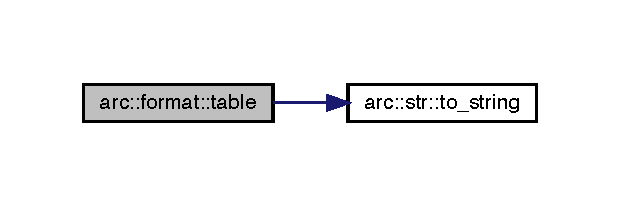
\includegraphics[width=297pt]{namespacearc_1_1format_a0c2871882ac6679e40c71a2176ddd529_cgraph}
\end{center}
\end{figure}

\hypertarget{namespacearc_1_1prop}{}\section{arc\+:\+:prop Namespace Reference}
\label{namespacearc_1_1prop}\index{arc\+::prop@{arc\+::prop}}


properties namespace  


\subsection*{Functions}
\begin{DoxyCompactItemize}
\item 
{\footnotesize template$<$typename C , typename T  = typename C\+::value\+\_\+type, typename I  = typename C\+::const\+\_\+iterator$>$ }\\bool \mbox{\hyperlink{namespacearc_1_1prop_a54974d0d56ee90909eac6cdd1b94cff5}{contains}} (const C \&cont\+\_\+, const T \&val\+\_\+) noexcept
\item 
{\footnotesize template$<$typename C , typename T  = typename C\+::value\+\_\+type, typename I  = typename C\+::const\+\_\+iterator$>$ }\\bool \mbox{\hyperlink{namespacearc_1_1prop_a026d439c76bdafd78b68875044d7b087}{ascending}} (const C \&cont\+\_\+) noexcept
\item 
{\footnotesize template$<$typename C , typename T  = typename C\+::value\+\_\+type, typename I  = typename C\+::const\+\_\+iterator$>$ }\\bool \mbox{\hyperlink{namespacearc_1_1prop_a156186f9684c79f4f28bb793af35f0bd}{descending}} (const C \&cont\+\_\+) noexcept
\item 
{\footnotesize template$<$typename C , typename T  = typename C\+::value\+\_\+type, typename I  = typename C\+::const\+\_\+iterator$>$ }\\bool \mbox{\hyperlink{namespacearc_1_1prop_a0b6cfeae4fa16eddbb6b7f1e9c355258}{monotonic}} (const C \&cont\+\_\+) noexcept
\item 
{\footnotesize template$<$typename C , typename T  = typename C\+::value\+\_\+type, typename I  = typename C\+::const\+\_\+iterator$>$ }\\bool \mbox{\hyperlink{namespacearc_1_1prop_aa5ffd8e519bbfe13d8b6c9b9ebf81855}{uniform}} (const C \&cont\+\_\+) noexcept
\item 
{\footnotesize template$<$typename C , typename T  = typename C\+::value\+\_\+type, typename I  = typename C\+::const\+\_\+iterator$>$ }\\bool \mbox{\hyperlink{namespacearc_1_1prop_a160eaff41b7223c20c03ca76ee4e1fb9}{within}} (const C \&cont\+\_\+, const T \&val\+\_\+) noexcept
\item 
{\footnotesize template$<$typename C , typename T  = typename C\+::value\+\_\+type, typename I  = typename C\+::const\+\_\+iterator$>$ }\\bool \mbox{\hyperlink{namespacearc_1_1prop_a965c4011bd27be186a9b63d69f27c4e4}{always\+\_\+less\+\_\+than}} (const C \&cont\+\_\+, const T \&limit\+\_\+) noexcept
\item 
{\footnotesize template$<$typename C , typename T  = typename C\+::value\+\_\+type, typename I  = typename C\+::const\+\_\+iterator$>$ }\\bool \mbox{\hyperlink{namespacearc_1_1prop_aa5ade88a045bf078e0dffe0418f133d5}{always\+\_\+less\+\_\+than\+\_\+or\+\_\+equal\+\_\+to}} (const C \&cont\+\_\+, const T \&limit\+\_\+) noexcept
\item 
{\footnotesize template$<$typename C , typename T  = typename C\+::value\+\_\+type, typename I  = typename C\+::const\+\_\+iterator$>$ }\\bool \mbox{\hyperlink{namespacearc_1_1prop_a0786e461abacc64a0479a9c29cebcfa9}{always\+\_\+greater\+\_\+than}} (const C \&cont\+\_\+, const T \&limit\+\_\+) noexcept
\item 
{\footnotesize template$<$typename C , typename T  = typename C\+::value\+\_\+type, typename I  = typename C\+::const\+\_\+iterator$>$ }\\bool \mbox{\hyperlink{namespacearc_1_1prop_a858cf86c6dc1c5ad0a337ac8adc7a787}{always\+\_\+greater\+\_\+than\+\_\+or\+\_\+equal\+\_\+to}} (const C \&cont\+\_\+, const T \&limit\+\_\+) noexcept
\end{DoxyCompactItemize}


\subsection{Detailed Description}
properties namespace 

\subsection{Function Documentation}
\mbox{\Hypertarget{namespacearc_1_1prop_a0786e461abacc64a0479a9c29cebcfa9}\label{namespacearc_1_1prop_a0786e461abacc64a0479a9c29cebcfa9}} 
\index{arc\+::prop@{arc\+::prop}!always\+\_\+greater\+\_\+than@{always\+\_\+greater\+\_\+than}}
\index{always\+\_\+greater\+\_\+than@{always\+\_\+greater\+\_\+than}!arc\+::prop@{arc\+::prop}}
\subsubsection{\texorpdfstring{always\+\_\+greater\+\_\+than()}{always\_greater\_than()}}
{\footnotesize\ttfamily template$<$typename C , typename T  = typename C\+::value\+\_\+type, typename I  = typename C\+::const\+\_\+iterator$>$ \\
bool arc\+::prop\+::always\+\_\+greater\+\_\+than (\begin{DoxyParamCaption}\item[{const C \&}]{cont\+\_\+,  }\item[{const T \&}]{limit\+\_\+ }\end{DoxyParamCaption})\hspace{0.3cm}{\ttfamily [inline]}, {\ttfamily [noexcept]}}

Determine if all elements of a container are greater than a given limit.


\begin{DoxyTemplParams}{Template Parameters}
{\em C} & Type of container. \\
\hline
{\em T} & Type stored by C. \\
\hline
{\em I} & Type of const iterator of C.\\
\hline
\end{DoxyTemplParams}

\begin{DoxyParams}{Parameters}
{\em cont\+\_\+} & Container to test. \\
\hline
{\em limit\+\_\+} & Limit to compare elements against.\\
\hline
\end{DoxyParams}
\begin{DoxyReturn}{Returns}
True if all elements are greater than the limit. 
\end{DoxyReturn}
\mbox{\Hypertarget{namespacearc_1_1prop_a858cf86c6dc1c5ad0a337ac8adc7a787}\label{namespacearc_1_1prop_a858cf86c6dc1c5ad0a337ac8adc7a787}} 
\index{arc\+::prop@{arc\+::prop}!always\+\_\+greater\+\_\+than\+\_\+or\+\_\+equal\+\_\+to@{always\+\_\+greater\+\_\+than\+\_\+or\+\_\+equal\+\_\+to}}
\index{always\+\_\+greater\+\_\+than\+\_\+or\+\_\+equal\+\_\+to@{always\+\_\+greater\+\_\+than\+\_\+or\+\_\+equal\+\_\+to}!arc\+::prop@{arc\+::prop}}
\subsubsection{\texorpdfstring{always\+\_\+greater\+\_\+than\+\_\+or\+\_\+equal\+\_\+to()}{always\_greater\_than\_or\_equal\_to()}}
{\footnotesize\ttfamily template$<$typename C , typename T  = typename C\+::value\+\_\+type, typename I  = typename C\+::const\+\_\+iterator$>$ \\
bool arc\+::prop\+::always\+\_\+greater\+\_\+than\+\_\+or\+\_\+equal\+\_\+to (\begin{DoxyParamCaption}\item[{const C \&}]{cont\+\_\+,  }\item[{const T \&}]{limit\+\_\+ }\end{DoxyParamCaption})\hspace{0.3cm}{\ttfamily [inline]}, {\ttfamily [noexcept]}}

Determine if all elements of a container are greater than, or equal to, a given limit.


\begin{DoxyTemplParams}{Template Parameters}
{\em C} & Type of container. \\
\hline
{\em T} & Type stored by C. \\
\hline
{\em I} & Type of const iterator of C.\\
\hline
\end{DoxyTemplParams}

\begin{DoxyParams}{Parameters}
{\em cont\+\_\+} & Container to test. \\
\hline
{\em limit\+\_\+} & Limit to compare elements against.\\
\hline
\end{DoxyParams}
\begin{DoxyReturn}{Returns}
True if all elements are greater than, or equal to, the limit. 
\end{DoxyReturn}
\mbox{\Hypertarget{namespacearc_1_1prop_a965c4011bd27be186a9b63d69f27c4e4}\label{namespacearc_1_1prop_a965c4011bd27be186a9b63d69f27c4e4}} 
\index{arc\+::prop@{arc\+::prop}!always\+\_\+less\+\_\+than@{always\+\_\+less\+\_\+than}}
\index{always\+\_\+less\+\_\+than@{always\+\_\+less\+\_\+than}!arc\+::prop@{arc\+::prop}}
\subsubsection{\texorpdfstring{always\+\_\+less\+\_\+than()}{always\_less\_than()}}
{\footnotesize\ttfamily template$<$typename C , typename T  = typename C\+::value\+\_\+type, typename I  = typename C\+::const\+\_\+iterator$>$ \\
bool arc\+::prop\+::always\+\_\+less\+\_\+than (\begin{DoxyParamCaption}\item[{const C \&}]{cont\+\_\+,  }\item[{const T \&}]{limit\+\_\+ }\end{DoxyParamCaption})\hspace{0.3cm}{\ttfamily [inline]}, {\ttfamily [noexcept]}}

Determine if all elements of a container are less than a given limit.


\begin{DoxyTemplParams}{Template Parameters}
{\em C} & Type of container. \\
\hline
{\em T} & Type stored by C. \\
\hline
{\em I} & Type of const iterator of C.\\
\hline
\end{DoxyTemplParams}

\begin{DoxyParams}{Parameters}
{\em cont\+\_\+} & Container to test. \\
\hline
{\em limit\+\_\+} & Limit to compare elements against.\\
\hline
\end{DoxyParams}
\begin{DoxyReturn}{Returns}
True if all elements are less than the limit. 
\end{DoxyReturn}
\mbox{\Hypertarget{namespacearc_1_1prop_aa5ade88a045bf078e0dffe0418f133d5}\label{namespacearc_1_1prop_aa5ade88a045bf078e0dffe0418f133d5}} 
\index{arc\+::prop@{arc\+::prop}!always\+\_\+less\+\_\+than\+\_\+or\+\_\+equal\+\_\+to@{always\+\_\+less\+\_\+than\+\_\+or\+\_\+equal\+\_\+to}}
\index{always\+\_\+less\+\_\+than\+\_\+or\+\_\+equal\+\_\+to@{always\+\_\+less\+\_\+than\+\_\+or\+\_\+equal\+\_\+to}!arc\+::prop@{arc\+::prop}}
\subsubsection{\texorpdfstring{always\+\_\+less\+\_\+than\+\_\+or\+\_\+equal\+\_\+to()}{always\_less\_than\_or\_equal\_to()}}
{\footnotesize\ttfamily template$<$typename C , typename T  = typename C\+::value\+\_\+type, typename I  = typename C\+::const\+\_\+iterator$>$ \\
bool arc\+::prop\+::always\+\_\+less\+\_\+than\+\_\+or\+\_\+equal\+\_\+to (\begin{DoxyParamCaption}\item[{const C \&}]{cont\+\_\+,  }\item[{const T \&}]{limit\+\_\+ }\end{DoxyParamCaption})\hspace{0.3cm}{\ttfamily [inline]}, {\ttfamily [noexcept]}}

Determine if all elements of a container are less than, or equal to, a given limit.


\begin{DoxyTemplParams}{Template Parameters}
{\em C} & Type of container. \\
\hline
{\em T} & Type stored by C. \\
\hline
{\em I} & Type of const iterator of C.\\
\hline
\end{DoxyTemplParams}

\begin{DoxyParams}{Parameters}
{\em cont\+\_\+} & Container to test. \\
\hline
{\em limit\+\_\+} & Limit to compare elements against.\\
\hline
\end{DoxyParams}
\begin{DoxyReturn}{Returns}
True if all elements are less than, or equal to, the limit. 
\end{DoxyReturn}
\mbox{\Hypertarget{namespacearc_1_1prop_a026d439c76bdafd78b68875044d7b087}\label{namespacearc_1_1prop_a026d439c76bdafd78b68875044d7b087}} 
\index{arc\+::prop@{arc\+::prop}!ascending@{ascending}}
\index{ascending@{ascending}!arc\+::prop@{arc\+::prop}}
\subsubsection{\texorpdfstring{ascending()}{ascending()}}
{\footnotesize\ttfamily template$<$typename C , typename T  = typename C\+::value\+\_\+type, typename I  = typename C\+::const\+\_\+iterator$>$ \\
bool arc\+::prop\+::ascending (\begin{DoxyParamCaption}\item[{const C \&}]{cont\+\_\+ }\end{DoxyParamCaption})\hspace{0.3cm}{\ttfamily [inline]}, {\ttfamily [noexcept]}}

Test if a container\textquotesingle{}s elements are sorted in ascending order. Container is still considered ascending if consecutive values are equal.


\begin{DoxyTemplParams}{Template Parameters}
{\em C} & Type of container. \\
\hline
{\em T} & Type stored by C. \\
\hline
{\em I} & Type of const iterator of C.\\
\hline
\end{DoxyTemplParams}

\begin{DoxyParams}{Parameters}
{\em cont\+\_\+} & Container to test.\\
\hline
\end{DoxyParams}
\begin{DoxyPrecond}{Precondition}
cont\+\_\+ must not be empty.
\end{DoxyPrecond}
\begin{DoxyReturn}{Returns}
True if the container\textquotesingle{}s elements are sorted in ascending order. 
\end{DoxyReturn}
Here is the caller graph for this function\+:\nopagebreak
\begin{figure}[H]
\begin{center}
\leavevmode
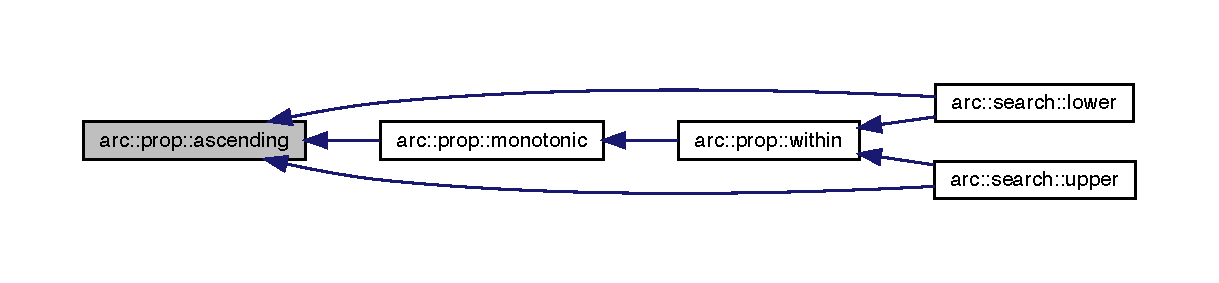
\includegraphics[width=350pt]{namespacearc_1_1prop_a026d439c76bdafd78b68875044d7b087_icgraph}
\end{center}
\end{figure}
\mbox{\Hypertarget{namespacearc_1_1prop_a54974d0d56ee90909eac6cdd1b94cff5}\label{namespacearc_1_1prop_a54974d0d56ee90909eac6cdd1b94cff5}} 
\index{arc\+::prop@{arc\+::prop}!contains@{contains}}
\index{contains@{contains}!arc\+::prop@{arc\+::prop}}
\subsubsection{\texorpdfstring{contains()}{contains()}}
{\footnotesize\ttfamily template$<$typename C , typename T  = typename C\+::value\+\_\+type, typename I  = typename C\+::const\+\_\+iterator$>$ \\
bool arc\+::prop\+::contains (\begin{DoxyParamCaption}\item[{const C \&}]{cont\+\_\+,  }\item[{const T \&}]{val\+\_\+ }\end{DoxyParamCaption})\hspace{0.3cm}{\ttfamily [inline]}, {\ttfamily [noexcept]}}

Determine if a container contains a value.


\begin{DoxyTemplParams}{Template Parameters}
{\em C} & Type of container. \\
\hline
{\em T} & Type stored by C. \\
\hline
{\em I} & Type of const iterator of C.\\
\hline
\end{DoxyTemplParams}

\begin{DoxyParams}{Parameters}
{\em cont\+\_\+} & Container to check. \\
\hline
{\em val\+\_\+} & Value to check container for.\\
\hline
\end{DoxyParams}
\begin{DoxyReturn}{Returns}
True if the container contains the value. 
\end{DoxyReturn}
\mbox{\Hypertarget{namespacearc_1_1prop_a156186f9684c79f4f28bb793af35f0bd}\label{namespacearc_1_1prop_a156186f9684c79f4f28bb793af35f0bd}} 
\index{arc\+::prop@{arc\+::prop}!descending@{descending}}
\index{descending@{descending}!arc\+::prop@{arc\+::prop}}
\subsubsection{\texorpdfstring{descending()}{descending()}}
{\footnotesize\ttfamily template$<$typename C , typename T  = typename C\+::value\+\_\+type, typename I  = typename C\+::const\+\_\+iterator$>$ \\
bool arc\+::prop\+::descending (\begin{DoxyParamCaption}\item[{const C \&}]{cont\+\_\+ }\end{DoxyParamCaption})\hspace{0.3cm}{\ttfamily [inline]}, {\ttfamily [noexcept]}}

Test if a container\textquotesingle{}s elements are sorted in descending order. Container is still considered descending if consecutive values are equal.


\begin{DoxyTemplParams}{Template Parameters}
{\em C} & Type of container. \\
\hline
{\em T} & Type stored by C. \\
\hline
{\em I} & Type of const iterator of C.\\
\hline
\end{DoxyTemplParams}

\begin{DoxyParams}{Parameters}
{\em cont\+\_\+} & Container to test.\\
\hline
\end{DoxyParams}
\begin{DoxyPrecond}{Precondition}
cont\+\_\+ must not be empty.
\end{DoxyPrecond}
\begin{DoxyReturn}{Returns}
True if the container\textquotesingle{}s elements are sorted in descending order. 
\end{DoxyReturn}
Here is the caller graph for this function\+:\nopagebreak
\begin{figure}[H]
\begin{center}
\leavevmode
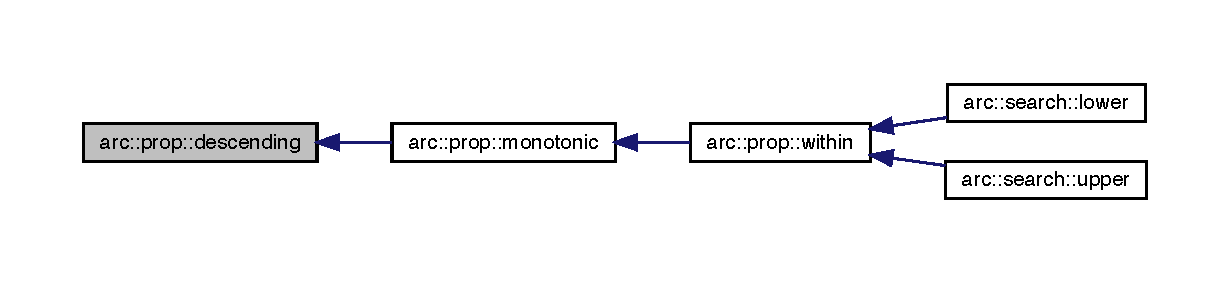
\includegraphics[width=350pt]{namespacearc_1_1prop_a156186f9684c79f4f28bb793af35f0bd_icgraph}
\end{center}
\end{figure}
\mbox{\Hypertarget{namespacearc_1_1prop_a0b6cfeae4fa16eddbb6b7f1e9c355258}\label{namespacearc_1_1prop_a0b6cfeae4fa16eddbb6b7f1e9c355258}} 
\index{arc\+::prop@{arc\+::prop}!monotonic@{monotonic}}
\index{monotonic@{monotonic}!arc\+::prop@{arc\+::prop}}
\subsubsection{\texorpdfstring{monotonic()}{monotonic()}}
{\footnotesize\ttfamily template$<$typename C , typename T  = typename C\+::value\+\_\+type, typename I  = typename C\+::const\+\_\+iterator$>$ \\
bool arc\+::prop\+::monotonic (\begin{DoxyParamCaption}\item[{const C \&}]{cont\+\_\+ }\end{DoxyParamCaption})\hspace{0.3cm}{\ttfamily [inline]}, {\ttfamily [noexcept]}}

Test if a container\textquotesingle{}s elements are sorted in monotonic order. Container is still considered monotonic if consecutive values are equal.


\begin{DoxyTemplParams}{Template Parameters}
{\em C} & Type of container. \\
\hline
{\em T} & Type stored by C. \\
\hline
{\em I} & Type of const iterator of C.\\
\hline
\end{DoxyTemplParams}

\begin{DoxyParams}{Parameters}
{\em cont\+\_\+} & Container to test.\\
\hline
\end{DoxyParams}
\begin{DoxyPrecond}{Precondition}
cont\+\_\+ must not be empty.
\end{DoxyPrecond}
\begin{DoxyReturn}{Returns}
True if the container\textquotesingle{}s elements are sorted in monotonic order. 
\end{DoxyReturn}
Here is the call graph for this function\+:\nopagebreak
\begin{figure}[H]
\begin{center}
\leavevmode
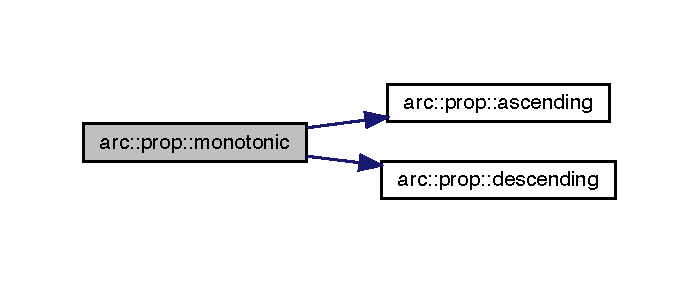
\includegraphics[width=335pt]{namespacearc_1_1prop_a0b6cfeae4fa16eddbb6b7f1e9c355258_cgraph}
\end{center}
\end{figure}
Here is the caller graph for this function\+:\nopagebreak
\begin{figure}[H]
\begin{center}
\leavevmode
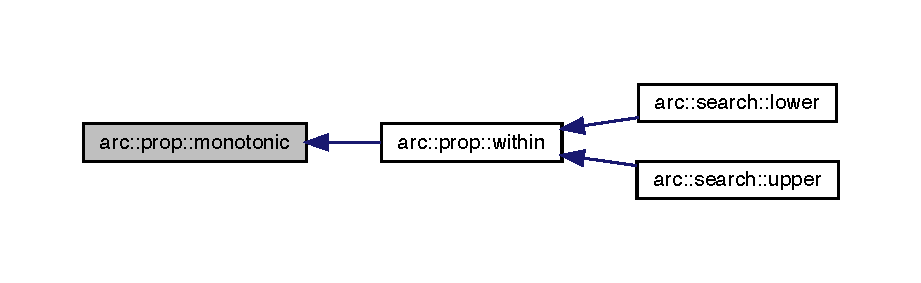
\includegraphics[width=350pt]{namespacearc_1_1prop_a0b6cfeae4fa16eddbb6b7f1e9c355258_icgraph}
\end{center}
\end{figure}
\mbox{\Hypertarget{namespacearc_1_1prop_aa5ffd8e519bbfe13d8b6c9b9ebf81855}\label{namespacearc_1_1prop_aa5ffd8e519bbfe13d8b6c9b9ebf81855}} 
\index{arc\+::prop@{arc\+::prop}!uniform@{uniform}}
\index{uniform@{uniform}!arc\+::prop@{arc\+::prop}}
\subsubsection{\texorpdfstring{uniform()}{uniform()}}
{\footnotesize\ttfamily template$<$typename C , typename T  = typename C\+::value\+\_\+type, typename I  = typename C\+::const\+\_\+iterator$>$ \\
bool arc\+::prop\+::uniform (\begin{DoxyParamCaption}\item[{const C \&}]{cont\+\_\+ }\end{DoxyParamCaption})\hspace{0.3cm}{\ttfamily [inline]}, {\ttfamily [noexcept]}}

Test if a container\textquotesingle{}s elements are uniformly spaced.


\begin{DoxyTemplParams}{Template Parameters}
{\em C} & Type of container. \\
\hline
{\em T} & Type stored by C. \\
\hline
{\em I} & Type of const iterator of C.\\
\hline
\end{DoxyTemplParams}

\begin{DoxyParams}{Parameters}
{\em cont\+\_\+} & Container to test.\\
\hline
\end{DoxyParams}
\begin{DoxyPrecond}{Precondition}
cont\+\_\+ must not be empty.
\end{DoxyPrecond}
\begin{DoxyReturn}{Returns}
True if the container\textquotesingle{}s elements are uniformly spaced. 
\end{DoxyReturn}
\mbox{\Hypertarget{namespacearc_1_1prop_a160eaff41b7223c20c03ca76ee4e1fb9}\label{namespacearc_1_1prop_a160eaff41b7223c20c03ca76ee4e1fb9}} 
\index{arc\+::prop@{arc\+::prop}!within@{within}}
\index{within@{within}!arc\+::prop@{arc\+::prop}}
\subsubsection{\texorpdfstring{within()}{within()}}
{\footnotesize\ttfamily template$<$typename C , typename T  = typename C\+::value\+\_\+type, typename I  = typename C\+::const\+\_\+iterator$>$ \\
bool arc\+::prop\+::within (\begin{DoxyParamCaption}\item[{const C \&}]{cont\+\_\+,  }\item[{const T \&}]{val\+\_\+ }\end{DoxyParamCaption})\hspace{0.3cm}{\ttfamily [inline]}, {\ttfamily [noexcept]}}

Determine if a value falls within the range of a container.


\begin{DoxyTemplParams}{Template Parameters}
{\em C} & Type of container. \\
\hline
{\em T} & Type stored by C. \\
\hline
{\em I} & Type of const iterator of C.\\
\hline
\end{DoxyTemplParams}

\begin{DoxyParams}{Parameters}
{\em cont\+\_\+} & Container to test. \\
\hline
{\em val\+\_\+} & Value to test.\\
\hline
\end{DoxyParams}
\begin{DoxyPrecond}{Precondition}
cont\+\_\+ must be monotonic.
\end{DoxyPrecond}
\begin{DoxyReturn}{Returns}
True if the value falls within the containers range. 
\end{DoxyReturn}
Here is the call graph for this function\+:\nopagebreak
\begin{figure}[H]
\begin{center}
\leavevmode
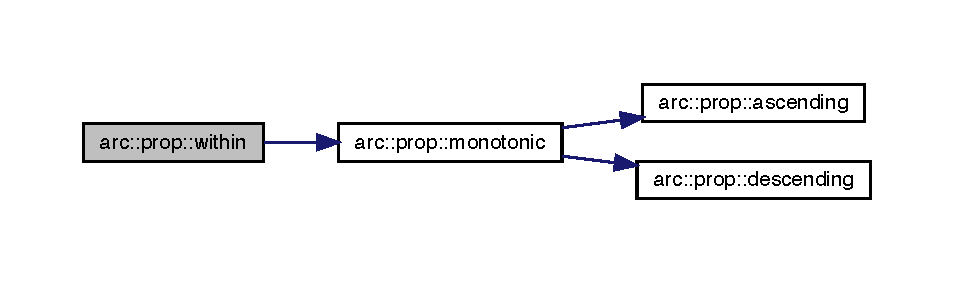
\includegraphics[width=350pt]{namespacearc_1_1prop_a160eaff41b7223c20c03ca76ee4e1fb9_cgraph}
\end{center}
\end{figure}
Here is the caller graph for this function\+:\nopagebreak
\begin{figure}[H]
\begin{center}
\leavevmode
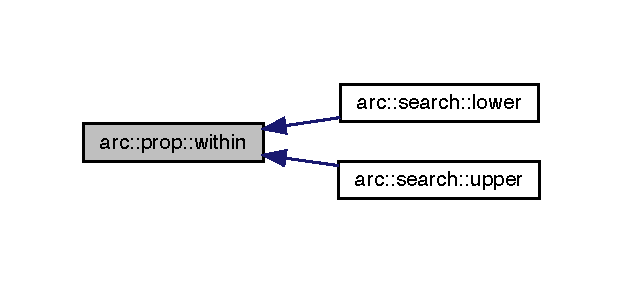
\includegraphics[width=299pt]{namespacearc_1_1prop_a160eaff41b7223c20c03ca76ee4e1fb9_icgraph}
\end{center}
\end{figure}

\hypertarget{namespacearc_1_1search}{}\section{arc\+:\+:search Namespace Reference}
\label{namespacearc_1_1search}\index{arc\+::search@{arc\+::search}}


search namespace  


\subsection*{Functions}
\begin{DoxyCompactItemize}
\item 
{\footnotesize template$<$typename C , typename T  = typename C\+::value\+\_\+type, typename I  = typename C\+::const\+\_\+iterator$>$ }\\size\+\_\+t \mbox{\hyperlink{namespacearc_1_1search_ae457da2cc210e1edfaf811bc83154f4b}{min\+\_\+index}} (const C \&cont\+\_\+) noexcept
\item 
{\footnotesize template$<$typename C , typename T  = typename C\+::value\+\_\+type, typename I  = typename C\+::const\+\_\+iterator$>$ }\\size\+\_\+t \mbox{\hyperlink{namespacearc_1_1search_aac33af22b716309501eaa7f5a10cc1d0}{max\+\_\+index}} (const C \&cont\+\_\+) noexcept
\item 
{\footnotesize template$<$typename C , typename T  = typename C\+::value\+\_\+type, typename I  = typename C\+::const\+\_\+iterator$>$ }\\T \mbox{\hyperlink{namespacearc_1_1search_a1cf0173ae1f8475d3b1652c006d5649d}{min}} (const C \&cont\+\_\+) noexcept
\item 
{\footnotesize template$<$typename C , typename T  = typename C\+::value\+\_\+type, typename I  = typename C\+::const\+\_\+iterator$>$ }\\T \mbox{\hyperlink{namespacearc_1_1search_ab5608d27962c637137d2c243213fa366}{max}} (const C \&cont\+\_\+) noexcept
\item 
{\footnotesize template$<$typename C , typename T  = typename C\+::value\+\_\+type, typename I  = typename C\+::const\+\_\+iterator$>$ }\\size\+\_\+t \mbox{\hyperlink{namespacearc_1_1search_ab5171637f0c917d6f387cb619a319ab5}{lower}} (const C \&cont\+\_\+, const T \&val\+\_\+) noexcept
\item 
{\footnotesize template$<$typename C , typename T  = typename C\+::value\+\_\+type, typename I  = typename C\+::const\+\_\+iterator$>$ }\\size\+\_\+t \mbox{\hyperlink{namespacearc_1_1search_a66f5d701ff409cb5e2673a4d5864cd11}{upper}} (const C \&cont\+\_\+, const T \&val\+\_\+) noexcept
\end{DoxyCompactItemize}


\subsection{Detailed Description}
search namespace 

\subsection{Function Documentation}
\mbox{\Hypertarget{namespacearc_1_1search_ab5171637f0c917d6f387cb619a319ab5}\label{namespacearc_1_1search_ab5171637f0c917d6f387cb619a319ab5}} 
\index{arc\+::search@{arc\+::search}!lower@{lower}}
\index{lower@{lower}!arc\+::search@{arc\+::search}}
\subsubsection{\texorpdfstring{lower()}{lower()}}
{\footnotesize\ttfamily template$<$typename C , typename T  = typename C\+::value\+\_\+type, typename I  = typename C\+::const\+\_\+iterator$>$ \\
size\+\_\+t arc\+::search\+::lower (\begin{DoxyParamCaption}\item[{const C \&}]{cont\+\_\+,  }\item[{const T \&}]{val\+\_\+ }\end{DoxyParamCaption})\hspace{0.3cm}{\ttfamily [inline]}, {\ttfamily [noexcept]}}

Find the index of the first element of the container that is not greater than or equal to the value given.


\begin{DoxyTemplParams}{Template Parameters}
{\em C} & Type of container. \\
\hline
{\em T} & Type stored by C. \\
\hline
{\em I} & Type of const iterator of C.\\
\hline
\end{DoxyTemplParams}

\begin{DoxyParams}{Parameters}
{\em cont\+\_\+} & Container to search. \\
\hline
{\em val\+\_\+} & Value to place.\\
\hline
\end{DoxyParams}
\begin{DoxyPrecond}{Precondition}
cont\+\_\+ must not be empty. 

cont\+\_\+ must be sorted in ascending order. 

val\+\_\+ must be within the range of cont\+\_\+.
\end{DoxyPrecond}
\begin{DoxyReturn}{Returns}
Index of the first element of the container that is not greater than or equal to the value given. 
\end{DoxyReturn}
Here is the call graph for this function\+:\nopagebreak
\begin{figure}[H]
\begin{center}
\leavevmode
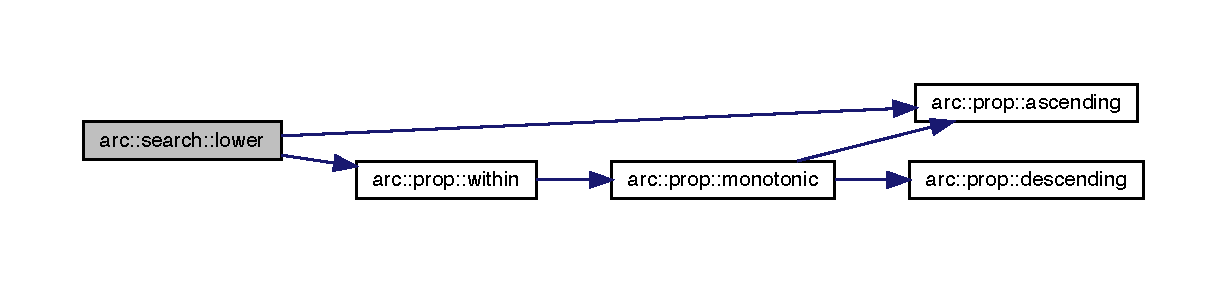
\includegraphics[width=350pt]{namespacearc_1_1search_ab5171637f0c917d6f387cb619a319ab5_cgraph}
\end{center}
\end{figure}
\mbox{\Hypertarget{namespacearc_1_1search_ab5608d27962c637137d2c243213fa366}\label{namespacearc_1_1search_ab5608d27962c637137d2c243213fa366}} 
\index{arc\+::search@{arc\+::search}!max@{max}}
\index{max@{max}!arc\+::search@{arc\+::search}}
\subsubsection{\texorpdfstring{max()}{max()}}
{\footnotesize\ttfamily template$<$typename C , typename T  = typename C\+::value\+\_\+type, typename I  = typename C\+::const\+\_\+iterator$>$ \\
T arc\+::search\+::max (\begin{DoxyParamCaption}\item[{const C \&}]{cont\+\_\+ }\end{DoxyParamCaption})\hspace{0.3cm}{\ttfamily [inline]}, {\ttfamily [noexcept]}}

Find the maximum element within a container.


\begin{DoxyTemplParams}{Template Parameters}
{\em C} & Type of container. \\
\hline
{\em T} & Type stored by C. \\
\hline
{\em I} & Type of const iterator of C.\\
\hline
\end{DoxyTemplParams}

\begin{DoxyParams}{Parameters}
{\em cont\+\_\+} & Container to determine the maximum element of.\\
\hline
\end{DoxyParams}
\begin{DoxyReturn}{Returns}
Value of the maximum element within the container. 
\end{DoxyReturn}
Here is the call graph for this function\+:\nopagebreak
\begin{figure}[H]
\begin{center}
\leavevmode
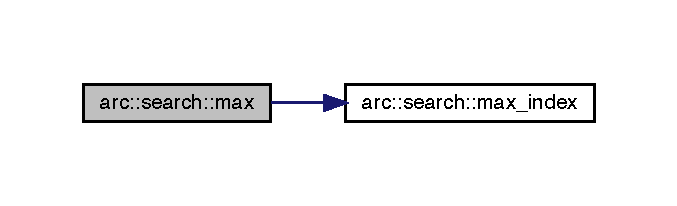
\includegraphics[width=325pt]{namespacearc_1_1search_ab5608d27962c637137d2c243213fa366_cgraph}
\end{center}
\end{figure}
\mbox{\Hypertarget{namespacearc_1_1search_aac33af22b716309501eaa7f5a10cc1d0}\label{namespacearc_1_1search_aac33af22b716309501eaa7f5a10cc1d0}} 
\index{arc\+::search@{arc\+::search}!max\+\_\+index@{max\+\_\+index}}
\index{max\+\_\+index@{max\+\_\+index}!arc\+::search@{arc\+::search}}
\subsubsection{\texorpdfstring{max\+\_\+index()}{max\_index()}}
{\footnotesize\ttfamily template$<$typename C , typename T  = typename C\+::value\+\_\+type, typename I  = typename C\+::const\+\_\+iterator$>$ \\
size\+\_\+t arc\+::search\+::max\+\_\+index (\begin{DoxyParamCaption}\item[{const C \&}]{cont\+\_\+ }\end{DoxyParamCaption})\hspace{0.3cm}{\ttfamily [inline]}, {\ttfamily [noexcept]}}

Find the index of the maximum element within a container.


\begin{DoxyTemplParams}{Template Parameters}
{\em C} & Type of container. \\
\hline
{\em T} & Type stored by C. \\
\hline
{\em I} & Type of const iterator of C.\\
\hline
\end{DoxyTemplParams}

\begin{DoxyParams}{Parameters}
{\em cont\+\_\+} & Container to determine the maximum element index of.\\
\hline
\end{DoxyParams}
\begin{DoxyPrecond}{Precondition}
cont\+\_\+ must not be empty.
\end{DoxyPrecond}
\begin{DoxyReturn}{Returns}
Index of the maximum element within the container. 
\end{DoxyReturn}
Here is the caller graph for this function\+:\nopagebreak
\begin{figure}[H]
\begin{center}
\leavevmode
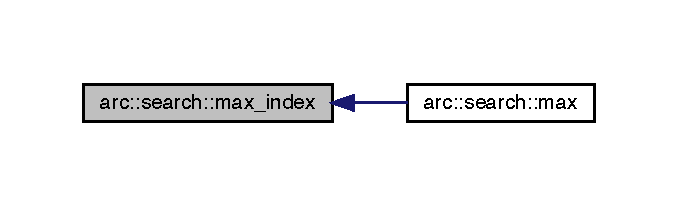
\includegraphics[width=325pt]{namespacearc_1_1search_aac33af22b716309501eaa7f5a10cc1d0_icgraph}
\end{center}
\end{figure}
\mbox{\Hypertarget{namespacearc_1_1search_a1cf0173ae1f8475d3b1652c006d5649d}\label{namespacearc_1_1search_a1cf0173ae1f8475d3b1652c006d5649d}} 
\index{arc\+::search@{arc\+::search}!min@{min}}
\index{min@{min}!arc\+::search@{arc\+::search}}
\subsubsection{\texorpdfstring{min()}{min()}}
{\footnotesize\ttfamily template$<$typename C , typename T  = typename C\+::value\+\_\+type, typename I  = typename C\+::const\+\_\+iterator$>$ \\
T arc\+::search\+::min (\begin{DoxyParamCaption}\item[{const C \&}]{cont\+\_\+ }\end{DoxyParamCaption})\hspace{0.3cm}{\ttfamily [inline]}, {\ttfamily [noexcept]}}

Find the minimum element within a container.


\begin{DoxyTemplParams}{Template Parameters}
{\em C} & Type of container. \\
\hline
{\em T} & Type stored by C. \\
\hline
{\em I} & Type of const iterator of C.\\
\hline
\end{DoxyTemplParams}

\begin{DoxyParams}{Parameters}
{\em cont\+\_\+} & Container to determine the minimum element of.\\
\hline
\end{DoxyParams}
\begin{DoxyPrecond}{Precondition}
cont\+\_\+ must not be empty.
\end{DoxyPrecond}
\begin{DoxyReturn}{Returns}
Value of the minimum element within the container. 
\end{DoxyReturn}
Here is the call graph for this function\+:\nopagebreak
\begin{figure}[H]
\begin{center}
\leavevmode
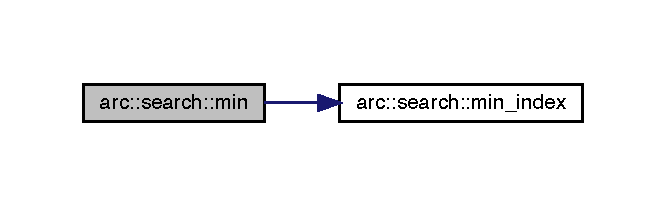
\includegraphics[width=320pt]{namespacearc_1_1search_a1cf0173ae1f8475d3b1652c006d5649d_cgraph}
\end{center}
\end{figure}
\mbox{\Hypertarget{namespacearc_1_1search_ae457da2cc210e1edfaf811bc83154f4b}\label{namespacearc_1_1search_ae457da2cc210e1edfaf811bc83154f4b}} 
\index{arc\+::search@{arc\+::search}!min\+\_\+index@{min\+\_\+index}}
\index{min\+\_\+index@{min\+\_\+index}!arc\+::search@{arc\+::search}}
\subsubsection{\texorpdfstring{min\+\_\+index()}{min\_index()}}
{\footnotesize\ttfamily template$<$typename C , typename T  = typename C\+::value\+\_\+type, typename I  = typename C\+::const\+\_\+iterator$>$ \\
size\+\_\+t arc\+::search\+::min\+\_\+index (\begin{DoxyParamCaption}\item[{const C \&}]{cont\+\_\+ }\end{DoxyParamCaption})\hspace{0.3cm}{\ttfamily [inline]}, {\ttfamily [noexcept]}}

Find the index of the minimum element within a container.


\begin{DoxyTemplParams}{Template Parameters}
{\em C} & Type of container. \\
\hline
{\em T} & Type stored by C. \\
\hline
{\em I} & Type of const iterator of C.\\
\hline
\end{DoxyTemplParams}

\begin{DoxyParams}{Parameters}
{\em cont\+\_\+} & Container to determine the minimum element index of.\\
\hline
\end{DoxyParams}
\begin{DoxyPrecond}{Precondition}
cont\+\_\+ must not be empty.
\end{DoxyPrecond}
\begin{DoxyReturn}{Returns}
Index of the minimum element within the container. 
\end{DoxyReturn}
Here is the caller graph for this function\+:\nopagebreak
\begin{figure}[H]
\begin{center}
\leavevmode
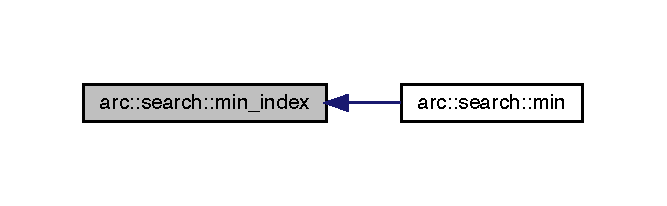
\includegraphics[width=320pt]{namespacearc_1_1search_ae457da2cc210e1edfaf811bc83154f4b_icgraph}
\end{center}
\end{figure}
\mbox{\Hypertarget{namespacearc_1_1search_a66f5d701ff409cb5e2673a4d5864cd11}\label{namespacearc_1_1search_a66f5d701ff409cb5e2673a4d5864cd11}} 
\index{arc\+::search@{arc\+::search}!upper@{upper}}
\index{upper@{upper}!arc\+::search@{arc\+::search}}
\subsubsection{\texorpdfstring{upper()}{upper()}}
{\footnotesize\ttfamily template$<$typename C , typename T  = typename C\+::value\+\_\+type, typename I  = typename C\+::const\+\_\+iterator$>$ \\
size\+\_\+t arc\+::search\+::upper (\begin{DoxyParamCaption}\item[{const C \&}]{cont\+\_\+,  }\item[{const T \&}]{val\+\_\+ }\end{DoxyParamCaption})\hspace{0.3cm}{\ttfamily [inline]}, {\ttfamily [noexcept]}}

Find the index of the first element of the container that is greater than the value given.


\begin{DoxyTemplParams}{Template Parameters}
{\em C} & Type of container. \\
\hline
{\em T} & Type stored by C. \\
\hline
{\em I} & Type of const iterator of C.\\
\hline
\end{DoxyTemplParams}

\begin{DoxyParams}{Parameters}
{\em cont\+\_\+} & Container to search. \\
\hline
{\em val\+\_\+} & Value to place.\\
\hline
\end{DoxyParams}
\begin{DoxyPrecond}{Precondition}
cont\+\_\+ must not be empty. 

cont\+\_\+ must be sorted in ascending order. 

val\+\_\+ must be within the range of cont\+\_\+.
\end{DoxyPrecond}
\begin{DoxyReturn}{Returns}
Index of the first element of the container that is greater than the value given. 
\end{DoxyReturn}
Here is the call graph for this function\+:\nopagebreak
\begin{figure}[H]
\begin{center}
\leavevmode
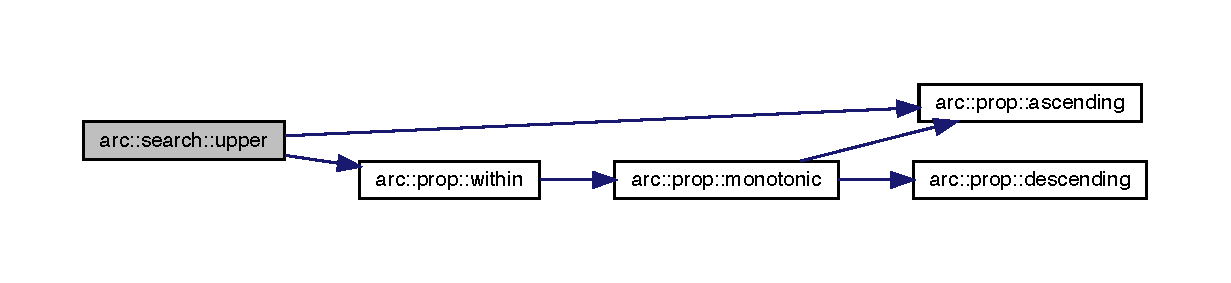
\includegraphics[width=350pt]{namespacearc_1_1search_a66f5d701ff409cb5e2673a4d5864cd11_cgraph}
\end{center}
\end{figure}

\hypertarget{namespacearc_1_1str}{}\section{arc\+:\+:str Namespace Reference}
\label{namespacearc_1_1str}\index{arc\+::str@{arc\+::str}}


string namespace  


\subsection*{Classes}
\begin{DoxyCompactItemize}
\item 
struct \mbox{\hyperlink{structarc_1_1str_1_1_tuple_to_string}{Tuple\+To\+String}}
\end{DoxyCompactItemize}
\subsection*{Functions}
\begin{DoxyCompactItemize}
\item 
{\footnotesize template$<$typename C , typename T  = typename C\+::value\+\_\+type, typename I  = typename C\+::const\+\_\+iterator$>$ }\\std\+::string \mbox{\hyperlink{namespacearc_1_1str_a53e4e5a084da03d5cc8ea2d4ee8ba7d0}{to\+\_\+string}} (const C \&cont\+\_\+, size\+\_\+t width\+\_\+=0, const std\+::string \&pre\+\_\+=\char`\"{}\{\char`\"{}, const std\+::string \&delim\+\_\+=\char`\"{}, \char`\"{}, const std\+::string \&post\+\_\+=\char`\"{}\}\char`\"{})
\item 
{\footnotesize template$<$typename A0 , typename A1 $>$ }\\std\+::string \mbox{\hyperlink{namespacearc_1_1str_a272000ff280c6447f036e80aeb3c3794}{to\+\_\+string}} (const std\+::pair$<$ A0, A1 $>$ \&pair\+\_\+, size\+\_\+t width\+\_\+=0, const std\+::string \&pre\+\_\+=\char`\"{}(\char`\"{}, const std\+::string \&delim\+\_\+=\char`\"{}, \char`\"{}, const std\+::string \&post\+\_\+=\char`\"{})\char`\"{})
\item 
{\footnotesize template$<$typename... A$>$ }\\std\+::string \mbox{\hyperlink{namespacearc_1_1str_ab73894966cf4d5672f5c86ba7a1a1465}{to\+\_\+string}} (const std\+::tuple$<$ A... $>$ \&tup\+\_\+, size\+\_\+t width\+\_\+=0, const std\+::string \&pre\+\_\+=\char`\"{}(\char`\"{}, const std\+::string \&delim\+\_\+=\char`\"{}, \char`\"{}, const std\+::string \&post\+\_\+=\char`\"{})\char`\"{})
\end{DoxyCompactItemize}


\subsection{Detailed Description}
string namespace 

\subsection{Function Documentation}
\mbox{\Hypertarget{namespacearc_1_1str_a53e4e5a084da03d5cc8ea2d4ee8ba7d0}\label{namespacearc_1_1str_a53e4e5a084da03d5cc8ea2d4ee8ba7d0}} 
\index{arc\+::str@{arc\+::str}!to\+\_\+string@{to\+\_\+string}}
\index{to\+\_\+string@{to\+\_\+string}!arc\+::str@{arc\+::str}}
\subsubsection{\texorpdfstring{to\+\_\+string()}{to\_string()}\hspace{0.1cm}{\footnotesize\ttfamily [1/3]}}
{\footnotesize\ttfamily template$<$typename C , typename T  = typename C\+::value\+\_\+type, typename I  = typename C\+::const\+\_\+iterator$>$ \\
std\+::string arc\+::str\+::to\+\_\+string (\begin{DoxyParamCaption}\item[{const C \&}]{cont\+\_\+,  }\item[{const size\+\_\+t}]{width\+\_\+,  }\item[{const std\+::string \&}]{pre\+\_\+,  }\item[{const std\+::string \&}]{delim\+\_\+,  }\item[{const std\+::string \&}]{post\+\_\+ }\end{DoxyParamCaption})\hspace{0.3cm}{\ttfamily [inline]}}

Form a container into a human-\/readable string.


\begin{DoxyTemplParams}{Template Parameters}
{\em C} & Type of container to print. \\
\hline
{\em T} & Type stored by C. \\
\hline
{\em I} & Type of const iterator of C.\\
\hline
\end{DoxyTemplParams}

\begin{DoxyParams}{Parameters}
{\em cont\+\_\+} & Container to print. \\
\hline
{\em width\+\_\+} & Print width allocated to each element. \\
\hline
{\em pre\+\_\+} & String prepended before the element data. \\
\hline
{\em delim\+\_\+} & Delimiter added between elements. \\
\hline
{\em post\+\_\+} & String appended after the element data.\\
\hline
\end{DoxyParams}
\begin{DoxyReturn}{Returns}
A human-\/readable string of the container. 
\end{DoxyReturn}
Here is the caller graph for this function\+:\nopagebreak
\begin{figure}[H]
\begin{center}
\leavevmode
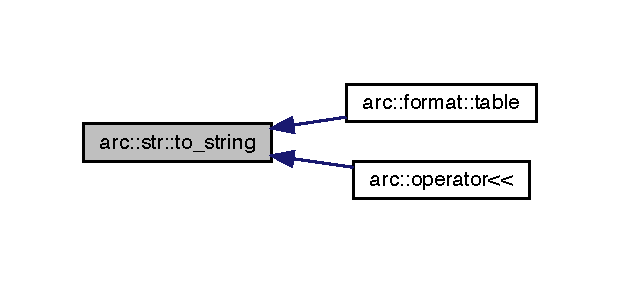
\includegraphics[width=297pt]{namespacearc_1_1str_a53e4e5a084da03d5cc8ea2d4ee8ba7d0_icgraph}
\end{center}
\end{figure}
\mbox{\Hypertarget{namespacearc_1_1str_a272000ff280c6447f036e80aeb3c3794}\label{namespacearc_1_1str_a272000ff280c6447f036e80aeb3c3794}} 
\index{arc\+::str@{arc\+::str}!to\+\_\+string@{to\+\_\+string}}
\index{to\+\_\+string@{to\+\_\+string}!arc\+::str@{arc\+::str}}
\subsubsection{\texorpdfstring{to\+\_\+string()}{to\_string()}\hspace{0.1cm}{\footnotesize\ttfamily [2/3]}}
{\footnotesize\ttfamily template$<$typename A0 , typename A1 $>$ \\
std\+::string arc\+::str\+::to\+\_\+string (\begin{DoxyParamCaption}\item[{const std\+::pair$<$ A0, A1 $>$ \&}]{pair\+\_\+,  }\item[{const size\+\_\+t}]{width\+\_\+,  }\item[{const std\+::string \&}]{pre\+\_\+,  }\item[{const std\+::string \&}]{delim\+\_\+,  }\item[{const std\+::string \&}]{post\+\_\+ }\end{DoxyParamCaption})\hspace{0.3cm}{\ttfamily [inline]}}

Form a pair into a human-\/readable string.


\begin{DoxyTemplParams}{Template Parameters}
{\em A0} & First type stored by pair. \\
\hline
{\em A1} & Second type stored by pair.\\
\hline
\end{DoxyTemplParams}

\begin{DoxyParams}{Parameters}
{\em pair\+\_\+} & Pair to print. \\
\hline
{\em width\+\_\+} & Print width allocated to each element. \\
\hline
{\em pre\+\_\+} & String prepended before the element data. \\
\hline
{\em delim\+\_\+} & Delimiter added between elements. \\
\hline
{\em post\+\_\+} & String appended after the element data.\\
\hline
\end{DoxyParams}
\begin{DoxyReturn}{Returns}
A human-\/readable string of the pair. 
\end{DoxyReturn}
\mbox{\Hypertarget{namespacearc_1_1str_ab73894966cf4d5672f5c86ba7a1a1465}\label{namespacearc_1_1str_ab73894966cf4d5672f5c86ba7a1a1465}} 
\index{arc\+::str@{arc\+::str}!to\+\_\+string@{to\+\_\+string}}
\index{to\+\_\+string@{to\+\_\+string}!arc\+::str@{arc\+::str}}
\subsubsection{\texorpdfstring{to\+\_\+string()}{to\_string()}\hspace{0.1cm}{\footnotesize\ttfamily [3/3]}}
{\footnotesize\ttfamily template$<$typename... A$>$ \\
std\+::string arc\+::str\+::to\+\_\+string (\begin{DoxyParamCaption}\item[{const std\+::tuple$<$ A... $>$ \&}]{tup\+\_\+,  }\item[{const size\+\_\+t}]{width\+\_\+,  }\item[{const std\+::string \&}]{pre\+\_\+,  }\item[{const std\+::string \&}]{delim\+\_\+,  }\item[{const std\+::string \&}]{post\+\_\+ }\end{DoxyParamCaption})\hspace{0.3cm}{\ttfamily [inline]}}

Form a tuple into a human-\/readable string. C++17 does not support template lambdas. Helper functor can be replaced with template lambda in C++2a.


\begin{DoxyTemplParams}{Template Parameters}
{\em A} & Types stored by the tuple.\\
\hline
\end{DoxyTemplParams}

\begin{DoxyParams}{Parameters}
{\em tup\+\_\+} & Tuple to print. \\
\hline
{\em width\+\_\+} & Print width allocated to each element. \\
\hline
{\em pre\+\_\+} & String prepended before the element data. \\
\hline
{\em delim\+\_\+} & Delimiter added between elements. \\
\hline
{\em post\+\_\+} & String appended after the element data.\\
\hline
\end{DoxyParams}
\begin{DoxyReturn}{Returns}
A human-\/readable string of the tuple. 
\end{DoxyReturn}
Here is the call graph for this function\+:\nopagebreak
\begin{figure}[H]
\begin{center}
\leavevmode
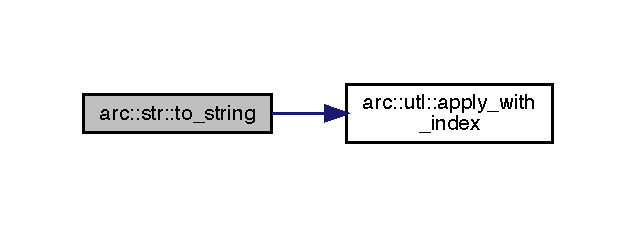
\includegraphics[width=305pt]{namespacearc_1_1str_ab73894966cf4d5672f5c86ba7a1a1465_cgraph}
\end{center}
\end{figure}

\hypertarget{namespacearc_1_1utl}{}\section{arc\+:\+:utl Namespace Reference}
\label{namespacearc_1_1utl}\index{arc\+::utl@{arc\+::utl}}


utility namespace  


\subsection*{Functions}
\begin{DoxyCompactItemize}
\item 
{\footnotesize template$<$typename C , typename T  = typename C\+::value\+\_\+type, typename I  = typename C\+::iterator, typename F $>$ }\\void \mbox{\hyperlink{namespacearc_1_1utl_a7e7db05c1cbc593d3bf9361621f763f3}{apply}} (C \&cont\+\_\+, F func\+\_\+) noexcept
\item 
{\footnotesize template$<$typename C , typename T  = typename C\+::value\+\_\+type, typename I  = typename C\+::cont\+\_\+iterator, typename F $>$ }\\void \mbox{\hyperlink{namespacearc_1_1utl_ae56f75d104c7bd4bd9abf350e349a694}{apply}} (const C \&cont\+\_\+, F func\+\_\+) noexcept
\item 
{\footnotesize template$<$typename C , typename T  = typename C\+::value\+\_\+type, typename I  = typename C\+::iterator, typename F $>$ }\\void \mbox{\hyperlink{namespacearc_1_1utl_a77de5138bbfff1ea74f34f3018361186}{apply\+\_\+with\+\_\+index}} (C \&cont\+\_\+, F func\+\_\+) noexcept
\item 
{\footnotesize template$<$typename C , typename T  = typename C\+::value\+\_\+type, typename I  = typename C\+::cont\+\_\+iterator, typename F $>$ }\\void \mbox{\hyperlink{namespacearc_1_1utl_a50e140f40e5a25a5fe253b94e6ab3403}{apply\+\_\+with\+\_\+index}} (const C \&cont\+\_\+, F func\+\_\+) noexcept
\item 
{\footnotesize template$<$typename A0 , typename A1 , typename F $>$ }\\void \mbox{\hyperlink{namespacearc_1_1utl_a77c34280ea834583a0a0563e2bdc549c}{apply}} (std\+::pair$<$ A0, A1 $>$ \&pair\+\_\+, F func\+\_\+)
\item 
{\footnotesize template$<$typename A0 , typename A1 , typename F $>$ }\\void \mbox{\hyperlink{namespacearc_1_1utl_a887b8885b94d550a15de9eef1a70fd0b}{apply}} (const std\+::pair$<$ A0, A1 $>$ \&pair\+\_\+, F func\+\_\+)
\item 
{\footnotesize template$<$typename A0 , typename A1 , typename F $>$ }\\void \mbox{\hyperlink{namespacearc_1_1utl_a97b916dd6673b3b3c190b15af1719b0a}{apply\+\_\+with\+\_\+index}} (std\+::pair$<$ A0, A1 $>$ \&pair\+\_\+, F func\+\_\+)
\item 
{\footnotesize template$<$typename A0 , typename A1 , typename F $>$ }\\void \mbox{\hyperlink{namespacearc_1_1utl_ad77a0481ab72232b49349532b96f80fc}{apply\+\_\+with\+\_\+index}} (const std\+::pair$<$ A0, A1 $>$ \&pair\+\_\+, F func\+\_\+)
\item 
{\footnotesize template$<$typename... A, typename F , size\+\_\+t... I$>$ }\\void \mbox{\hyperlink{namespacearc_1_1utl_a5421e6de5c0a785ee70d9546d6ef0c41}{apply\+\_\+to\+\_\+each}} (std\+::tuple$<$ A... $>$ \&tuple\+\_\+, F func\+\_\+, std\+::index\+\_\+sequence$<$ I... $>$)
\item 
{\footnotesize template$<$typename... A, typename F $>$ }\\void \mbox{\hyperlink{namespacearc_1_1utl_af64bed0e9e6ac7220d393a1bb62f4bff}{apply}} (std\+::tuple$<$ A... $>$ \&tuple\+\_\+, F func\+\_\+)
\item 
{\footnotesize template$<$typename... A, typename F , size\+\_\+t... I$>$ }\\void \mbox{\hyperlink{namespacearc_1_1utl_acf59dac8c2f5eea5a6aa9875db3b07f8}{apply\+\_\+to\+\_\+each}} (const std\+::tuple$<$ A... $>$ \&tuple\+\_\+, F func\+\_\+, std\+::index\+\_\+sequence$<$ I... $>$)
\item 
{\footnotesize template$<$typename... A, typename F $>$ }\\void \mbox{\hyperlink{namespacearc_1_1utl_a6dadc719c6540032592f36b5c14cae27}{apply}} (const std\+::tuple$<$ A... $>$ \&tuple\+\_\+, F func\+\_\+)
\item 
{\footnotesize template$<$typename... A, typename F , size\+\_\+t... I$>$ }\\void \mbox{\hyperlink{namespacearc_1_1utl_a0bc38a64f17e53212169cae0a6eb23bb}{apply\+\_\+to\+\_\+each\+\_\+with\+\_\+index}} (std\+::tuple$<$ A... $>$ \&tuple\+\_\+, F func\+\_\+, std\+::index\+\_\+sequence$<$ I... $>$)
\item 
{\footnotesize template$<$typename... A, typename F $>$ }\\void \mbox{\hyperlink{namespacearc_1_1utl_a2658c84859917c434ff3a7f667b21eca}{apply\+\_\+with\+\_\+index}} (std\+::tuple$<$ A... $>$ \&tuple\+\_\+, F func\+\_\+)
\item 
{\footnotesize template$<$typename... A, typename F , size\+\_\+t... I$>$ }\\void \mbox{\hyperlink{namespacearc_1_1utl_a6330262543d471ad23a1a70ea3a47b53}{apply\+\_\+to\+\_\+each\+\_\+with\+\_\+index}} (const std\+::tuple$<$ A... $>$ \&tuple\+\_\+, F func\+\_\+, std\+::index\+\_\+sequence$<$ I... $>$)
\item 
{\footnotesize template$<$typename... A, typename F $>$ }\\void \mbox{\hyperlink{namespacearc_1_1utl_ae57e12a4fd6beeb3a1a40bfd461c3a87}{apply\+\_\+with\+\_\+index}} (const std\+::tuple$<$ A... $>$ \&tuple\+\_\+, F func\+\_\+)
\end{DoxyCompactItemize}


\subsection{Detailed Description}
utility namespace 

\subsection{Function Documentation}
\mbox{\Hypertarget{namespacearc_1_1utl_a7e7db05c1cbc593d3bf9361621f763f3}\label{namespacearc_1_1utl_a7e7db05c1cbc593d3bf9361621f763f3}} 
\index{arc\+::utl@{arc\+::utl}!apply@{apply}}
\index{apply@{apply}!arc\+::utl@{arc\+::utl}}
\subsubsection{\texorpdfstring{apply()}{apply()}\hspace{0.1cm}{\footnotesize\ttfamily [1/6]}}
{\footnotesize\ttfamily template$<$typename C , typename T  = typename C\+::value\+\_\+type, typename I  = typename C\+::iterator, typename F $>$ \\
void arc\+::utl\+::apply (\begin{DoxyParamCaption}\item[{C \&}]{cont\+\_\+,  }\item[{F}]{func\+\_\+ }\end{DoxyParamCaption})\hspace{0.3cm}{\ttfamily [inline]}, {\ttfamily [noexcept]}}

Apply a given functor to each element of a container.


\begin{DoxyTemplParams}{Template Parameters}
{\em C} & Type of container. \\
\hline
{\em T} & Type stored by C. \\
\hline
{\em I} & Type of const iterator of C. \\
\hline
{\em F} & Type of functor to be applied.\\
\hline
\end{DoxyTemplParams}

\begin{DoxyParams}{Parameters}
{\em cont\+\_\+} & Container to be applied to. \\
\hline
{\em func\+\_\+} & Functor to be applied. \\
\hline
\end{DoxyParams}
\mbox{\Hypertarget{namespacearc_1_1utl_a77c34280ea834583a0a0563e2bdc549c}\label{namespacearc_1_1utl_a77c34280ea834583a0a0563e2bdc549c}} 
\index{arc\+::utl@{arc\+::utl}!apply@{apply}}
\index{apply@{apply}!arc\+::utl@{arc\+::utl}}
\subsubsection{\texorpdfstring{apply()}{apply()}\hspace{0.1cm}{\footnotesize\ttfamily [2/6]}}
{\footnotesize\ttfamily template$<$typename A0 , typename A1 , typename F $>$ \\
void arc\+::utl\+::apply (\begin{DoxyParamCaption}\item[{std\+::pair$<$ A0, A1 $>$ \&}]{pair\+\_\+,  }\item[{F}]{func\+\_\+ }\end{DoxyParamCaption})}

Call a functor on each element of a pair.


\begin{DoxyTemplParams}{Template Parameters}
{\em A0} & First type stored by the pair. \\
\hline
{\em A1} & Second type stored by the pair. \\
\hline
{\em F} & Type of functor to be applied.\\
\hline
\end{DoxyTemplParams}

\begin{DoxyParams}{Parameters}
{\em pair\+\_\+} & Pair to be applied to. \\
\hline
{\em func\+\_\+} & Functor to be applied. \\
\hline
\end{DoxyParams}
\mbox{\Hypertarget{namespacearc_1_1utl_ae56f75d104c7bd4bd9abf350e349a694}\label{namespacearc_1_1utl_ae56f75d104c7bd4bd9abf350e349a694}} 
\index{arc\+::utl@{arc\+::utl}!apply@{apply}}
\index{apply@{apply}!arc\+::utl@{arc\+::utl}}
\subsubsection{\texorpdfstring{apply()}{apply()}\hspace{0.1cm}{\footnotesize\ttfamily [3/6]}}
{\footnotesize\ttfamily template$<$typename C , typename T  = typename C\+::value\+\_\+type, typename I  = typename C\+::cont\+\_\+iterator, typename F $>$ \\
void arc\+::utl\+::apply (\begin{DoxyParamCaption}\item[{const C \&}]{cont\+\_\+,  }\item[{F}]{func\+\_\+ }\end{DoxyParamCaption})\hspace{0.3cm}{\ttfamily [inline]}, {\ttfamily [noexcept]}}

Apply a given functor to each element of a const container.


\begin{DoxyTemplParams}{Template Parameters}
{\em C} & Type of container. \\
\hline
{\em T} & Type stored by C. \\
\hline
{\em I} & Type of const iterator of C. \\
\hline
{\em F} & Type of functor to be applied.\\
\hline
\end{DoxyTemplParams}

\begin{DoxyParams}{Parameters}
{\em cont\+\_\+} & Container to be applied to. \\
\hline
{\em func\+\_\+} & Functor to be applied. \\
\hline
\end{DoxyParams}
\mbox{\Hypertarget{namespacearc_1_1utl_a887b8885b94d550a15de9eef1a70fd0b}\label{namespacearc_1_1utl_a887b8885b94d550a15de9eef1a70fd0b}} 
\index{arc\+::utl@{arc\+::utl}!apply@{apply}}
\index{apply@{apply}!arc\+::utl@{arc\+::utl}}
\subsubsection{\texorpdfstring{apply()}{apply()}\hspace{0.1cm}{\footnotesize\ttfamily [4/6]}}
{\footnotesize\ttfamily template$<$typename A0 , typename A1 , typename F $>$ \\
void arc\+::utl\+::apply (\begin{DoxyParamCaption}\item[{const std\+::pair$<$ A0, A1 $>$ \&}]{pair\+\_\+,  }\item[{F}]{func\+\_\+ }\end{DoxyParamCaption})}

Call a functor on each element of a const pair.


\begin{DoxyTemplParams}{Template Parameters}
{\em A0} & First type stored by the pair. \\
\hline
{\em A1} & Second type stored by the pair. \\
\hline
{\em F} & Type of functor to be applied.\\
\hline
\end{DoxyTemplParams}

\begin{DoxyParams}{Parameters}
{\em pair\+\_\+} & Pair to be applied to. \\
\hline
{\em func\+\_\+} & Functor to be applied. \\
\hline
\end{DoxyParams}
\mbox{\Hypertarget{namespacearc_1_1utl_af64bed0e9e6ac7220d393a1bb62f4bff}\label{namespacearc_1_1utl_af64bed0e9e6ac7220d393a1bb62f4bff}} 
\index{arc\+::utl@{arc\+::utl}!apply@{apply}}
\index{apply@{apply}!arc\+::utl@{arc\+::utl}}
\subsubsection{\texorpdfstring{apply()}{apply()}\hspace{0.1cm}{\footnotesize\ttfamily [5/6]}}
{\footnotesize\ttfamily template$<$typename... A, typename F $>$ \\
void arc\+::utl\+::apply (\begin{DoxyParamCaption}\item[{std\+::tuple$<$ A... $>$ \&}]{tuple\+\_\+,  }\item[{F}]{func\+\_\+ }\end{DoxyParamCaption})}

Apply a given functor to each element of a tuple.


\begin{DoxyTemplParams}{Template Parameters}
{\em A} & Types stored by the tuple. \\
\hline
{\em F} & Type of functor to be applied.\\
\hline
\end{DoxyTemplParams}

\begin{DoxyParams}{Parameters}
{\em tuple\+\_\+} & Tuple to be applied to. \\
\hline
{\em func\+\_\+} & Functor to be applied. \\
\hline
\end{DoxyParams}
Here is the call graph for this function\+:\nopagebreak
\begin{figure}[H]
\begin{center}
\leavevmode
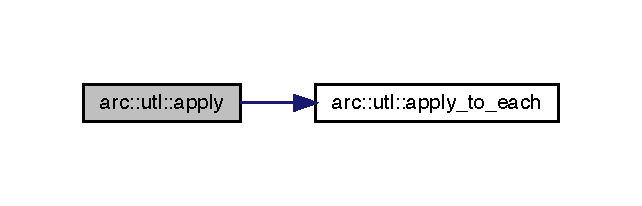
\includegraphics[width=308pt]{namespacearc_1_1utl_af64bed0e9e6ac7220d393a1bb62f4bff_cgraph}
\end{center}
\end{figure}
\mbox{\Hypertarget{namespacearc_1_1utl_a6dadc719c6540032592f36b5c14cae27}\label{namespacearc_1_1utl_a6dadc719c6540032592f36b5c14cae27}} 
\index{arc\+::utl@{arc\+::utl}!apply@{apply}}
\index{apply@{apply}!arc\+::utl@{arc\+::utl}}
\subsubsection{\texorpdfstring{apply()}{apply()}\hspace{0.1cm}{\footnotesize\ttfamily [6/6]}}
{\footnotesize\ttfamily template$<$typename... A, typename F $>$ \\
void arc\+::utl\+::apply (\begin{DoxyParamCaption}\item[{const std\+::tuple$<$ A... $>$ \&}]{tuple\+\_\+,  }\item[{F}]{func\+\_\+ }\end{DoxyParamCaption})}

Apply a given functor to each element of a const tuple.


\begin{DoxyTemplParams}{Template Parameters}
{\em A} & Types stored by the tuple. \\
\hline
{\em F} & Type of functor to be applied.\\
\hline
\end{DoxyTemplParams}

\begin{DoxyParams}{Parameters}
{\em tuple\+\_\+} & Tuple to be applied to. \\
\hline
{\em func\+\_\+} & Functor to be applied. \\
\hline
\end{DoxyParams}
Here is the call graph for this function\+:\nopagebreak
\begin{figure}[H]
\begin{center}
\leavevmode
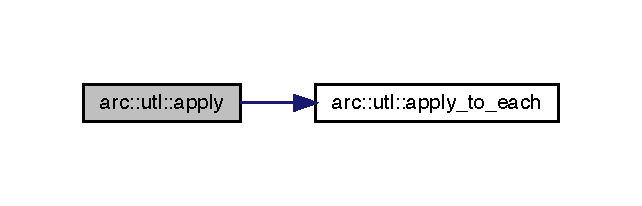
\includegraphics[width=308pt]{namespacearc_1_1utl_a6dadc719c6540032592f36b5c14cae27_cgraph}
\end{center}
\end{figure}
\mbox{\Hypertarget{namespacearc_1_1utl_a5421e6de5c0a785ee70d9546d6ef0c41}\label{namespacearc_1_1utl_a5421e6de5c0a785ee70d9546d6ef0c41}} 
\index{arc\+::utl@{arc\+::utl}!apply\+\_\+to\+\_\+each@{apply\+\_\+to\+\_\+each}}
\index{apply\+\_\+to\+\_\+each@{apply\+\_\+to\+\_\+each}!arc\+::utl@{arc\+::utl}}
\subsubsection{\texorpdfstring{apply\+\_\+to\+\_\+each()}{apply\_to\_each()}\hspace{0.1cm}{\footnotesize\ttfamily [1/2]}}
{\footnotesize\ttfamily template$<$typename... A, typename F , size\+\_\+t... I$>$ \\
void arc\+::utl\+::apply\+\_\+to\+\_\+each (\begin{DoxyParamCaption}\item[{std\+::tuple$<$ A... $>$ \&}]{tuple\+\_\+,  }\item[{F}]{func\+\_\+,  }\item[{std\+::index\+\_\+sequence$<$ I... $>$}]{ }\end{DoxyParamCaption})}

Apply helper function. Call a functor on each element of a const tuple.


\begin{DoxyTemplParams}{Template Parameters}
{\em A} & Types stored by the tuple. \\
\hline
{\em F} & Type of functor to be applied. \\
\hline
{\em I} & Indices of the tuple.\\
\hline
\end{DoxyTemplParams}

\begin{DoxyParams}{Parameters}
{\em tuple\+\_\+} & Tuple to be applied to. \\
\hline
{\em func\+\_\+} & Functor to be applied. \\
\hline
\end{DoxyParams}
Here is the caller graph for this function\+:\nopagebreak
\begin{figure}[H]
\begin{center}
\leavevmode
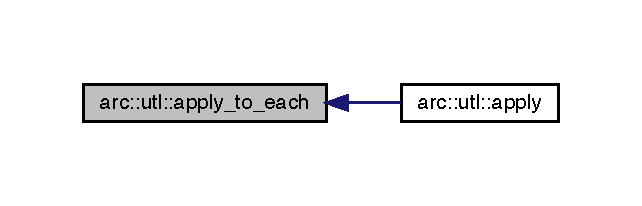
\includegraphics[width=308pt]{namespacearc_1_1utl_a5421e6de5c0a785ee70d9546d6ef0c41_icgraph}
\end{center}
\end{figure}
\mbox{\Hypertarget{namespacearc_1_1utl_acf59dac8c2f5eea5a6aa9875db3b07f8}\label{namespacearc_1_1utl_acf59dac8c2f5eea5a6aa9875db3b07f8}} 
\index{arc\+::utl@{arc\+::utl}!apply\+\_\+to\+\_\+each@{apply\+\_\+to\+\_\+each}}
\index{apply\+\_\+to\+\_\+each@{apply\+\_\+to\+\_\+each}!arc\+::utl@{arc\+::utl}}
\subsubsection{\texorpdfstring{apply\+\_\+to\+\_\+each()}{apply\_to\_each()}\hspace{0.1cm}{\footnotesize\ttfamily [2/2]}}
{\footnotesize\ttfamily template$<$typename... A, typename F , size\+\_\+t... I$>$ \\
void arc\+::utl\+::apply\+\_\+to\+\_\+each (\begin{DoxyParamCaption}\item[{const std\+::tuple$<$ A... $>$ \&}]{tuple\+\_\+,  }\item[{F}]{func\+\_\+,  }\item[{std\+::index\+\_\+sequence$<$ I... $>$}]{ }\end{DoxyParamCaption})}

Apply helper function. Call a functor on each element of a tuple.


\begin{DoxyTemplParams}{Template Parameters}
{\em A} & Types stored by the tuple. \\
\hline
{\em F} & Type of functor to be applied. \\
\hline
{\em I} & Indices of the tuple.\\
\hline
\end{DoxyTemplParams}

\begin{DoxyParams}{Parameters}
{\em tuple\+\_\+} & Tuple to be applied to. \\
\hline
{\em func\+\_\+} & Functor to be applied. \\
\hline
\end{DoxyParams}
\mbox{\Hypertarget{namespacearc_1_1utl_a0bc38a64f17e53212169cae0a6eb23bb}\label{namespacearc_1_1utl_a0bc38a64f17e53212169cae0a6eb23bb}} 
\index{arc\+::utl@{arc\+::utl}!apply\+\_\+to\+\_\+each\+\_\+with\+\_\+index@{apply\+\_\+to\+\_\+each\+\_\+with\+\_\+index}}
\index{apply\+\_\+to\+\_\+each\+\_\+with\+\_\+index@{apply\+\_\+to\+\_\+each\+\_\+with\+\_\+index}!arc\+::utl@{arc\+::utl}}
\subsubsection{\texorpdfstring{apply\+\_\+to\+\_\+each\+\_\+with\+\_\+index()}{apply\_to\_each\_with\_index()}\hspace{0.1cm}{\footnotesize\ttfamily [1/2]}}
{\footnotesize\ttfamily template$<$typename... A, typename F , size\+\_\+t... I$>$ \\
void arc\+::utl\+::apply\+\_\+to\+\_\+each\+\_\+with\+\_\+index (\begin{DoxyParamCaption}\item[{std\+::tuple$<$ A... $>$ \&}]{tuple\+\_\+,  }\item[{F}]{func\+\_\+,  }\item[{std\+::index\+\_\+sequence$<$ I... $>$}]{seq\+\_\+ }\end{DoxyParamCaption})}

Apply with index helper function. Call a functor on each element of a tuple. Provide the current tuple index and the total number of tuple types.


\begin{DoxyTemplParams}{Template Parameters}
{\em A} & Types stored by the tuple. \\
\hline
{\em F} & Type of functor to be applied. \\
\hline
{\em I} & Indices of the tuple.\\
\hline
\end{DoxyTemplParams}

\begin{DoxyParams}{Parameters}
{\em tuple\+\_\+} & Tuple to be applied to. \\
\hline
{\em func\+\_\+} & Functor to be applied. \\
\hline
{\em seq\+\_\+} & Sequence of tuple indices. \\
\hline
\end{DoxyParams}
Here is the caller graph for this function\+:\nopagebreak
\begin{figure}[H]
\begin{center}
\leavevmode
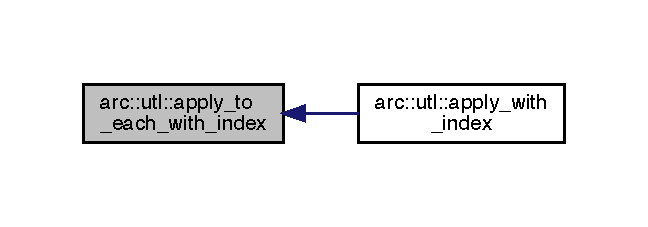
\includegraphics[width=311pt]{namespacearc_1_1utl_a0bc38a64f17e53212169cae0a6eb23bb_icgraph}
\end{center}
\end{figure}
\mbox{\Hypertarget{namespacearc_1_1utl_a6330262543d471ad23a1a70ea3a47b53}\label{namespacearc_1_1utl_a6330262543d471ad23a1a70ea3a47b53}} 
\index{arc\+::utl@{arc\+::utl}!apply\+\_\+to\+\_\+each\+\_\+with\+\_\+index@{apply\+\_\+to\+\_\+each\+\_\+with\+\_\+index}}
\index{apply\+\_\+to\+\_\+each\+\_\+with\+\_\+index@{apply\+\_\+to\+\_\+each\+\_\+with\+\_\+index}!arc\+::utl@{arc\+::utl}}
\subsubsection{\texorpdfstring{apply\+\_\+to\+\_\+each\+\_\+with\+\_\+index()}{apply\_to\_each\_with\_index()}\hspace{0.1cm}{\footnotesize\ttfamily [2/2]}}
{\footnotesize\ttfamily template$<$typename... A, typename F , size\+\_\+t... I$>$ \\
void arc\+::utl\+::apply\+\_\+to\+\_\+each\+\_\+with\+\_\+index (\begin{DoxyParamCaption}\item[{const std\+::tuple$<$ A... $>$ \&}]{tuple\+\_\+,  }\item[{F}]{func\+\_\+,  }\item[{std\+::index\+\_\+sequence$<$ I... $>$}]{seq\+\_\+ }\end{DoxyParamCaption})}

Apply with index helper function. Call a functor on each element of a const tuple. Provide the current tuple index and the total number of tuple types.


\begin{DoxyTemplParams}{Template Parameters}
{\em A} & Types stored by the tuple. \\
\hline
{\em F} & Type of functor to be applied. \\
\hline
{\em I} & Indices of the tuple.\\
\hline
\end{DoxyTemplParams}

\begin{DoxyParams}{Parameters}
{\em tuple\+\_\+} & Tuple to be applied to. \\
\hline
{\em func\+\_\+} & Functor to be applied. \\
\hline
{\em seq\+\_\+} & Sequence of tuple indices. \\
\hline
\end{DoxyParams}
\mbox{\Hypertarget{namespacearc_1_1utl_a97b916dd6673b3b3c190b15af1719b0a}\label{namespacearc_1_1utl_a97b916dd6673b3b3c190b15af1719b0a}} 
\index{arc\+::utl@{arc\+::utl}!apply\+\_\+with\+\_\+index@{apply\+\_\+with\+\_\+index}}
\index{apply\+\_\+with\+\_\+index@{apply\+\_\+with\+\_\+index}!arc\+::utl@{arc\+::utl}}
\subsubsection{\texorpdfstring{apply\+\_\+with\+\_\+index()}{apply\_with\_index()}\hspace{0.1cm}{\footnotesize\ttfamily [1/6]}}
{\footnotesize\ttfamily template$<$typename A0 , typename A1 , typename F $>$ \\
void arc\+::utl\+::apply\+\_\+with\+\_\+index (\begin{DoxyParamCaption}\item[{std\+::pair$<$ A0, A1 $>$ \&}]{pair\+\_\+,  }\item[{F}]{func\+\_\+ }\end{DoxyParamCaption})}

Call a functor on each element of a pair. Provide the pair index and the total number of pair types.


\begin{DoxyTemplParams}{Template Parameters}
{\em A0} & First type stored by the pair. \\
\hline
{\em A1} & Second type stored by the pair. \\
\hline
{\em F} & Type of functor to be applied.\\
\hline
\end{DoxyTemplParams}

\begin{DoxyParams}{Parameters}
{\em pair\+\_\+} & Pair to be applied to. \\
\hline
{\em func\+\_\+} & Functor to be applied. \\
\hline
\end{DoxyParams}
\mbox{\Hypertarget{namespacearc_1_1utl_a77de5138bbfff1ea74f34f3018361186}\label{namespacearc_1_1utl_a77de5138bbfff1ea74f34f3018361186}} 
\index{arc\+::utl@{arc\+::utl}!apply\+\_\+with\+\_\+index@{apply\+\_\+with\+\_\+index}}
\index{apply\+\_\+with\+\_\+index@{apply\+\_\+with\+\_\+index}!arc\+::utl@{arc\+::utl}}
\subsubsection{\texorpdfstring{apply\+\_\+with\+\_\+index()}{apply\_with\_index()}\hspace{0.1cm}{\footnotesize\ttfamily [2/6]}}
{\footnotesize\ttfamily template$<$typename C , typename T  = typename C\+::value\+\_\+type, typename I  = typename C\+::iterator, typename F $>$ \\
void arc\+::utl\+::apply\+\_\+with\+\_\+index (\begin{DoxyParamCaption}\item[{C \&}]{cont\+\_\+,  }\item[{F}]{func\+\_\+ }\end{DoxyParamCaption})\hspace{0.3cm}{\ttfamily [inline]}, {\ttfamily [noexcept]}}

Apply a given functor to each element of a container. Provide the current element index and the total number of elements.


\begin{DoxyTemplParams}{Template Parameters}
{\em C} & Type of container. \\
\hline
{\em T} & Type stored by C. \\
\hline
{\em I} & Type of const iterator of C. \\
\hline
{\em F} & Type of functor to be applied.\\
\hline
\end{DoxyTemplParams}

\begin{DoxyParams}{Parameters}
{\em cont\+\_\+} & Container to be applied to. \\
\hline
{\em func\+\_\+} & Functor to be applied. \\
\hline
\end{DoxyParams}
Here is the caller graph for this function\+:\nopagebreak
\begin{figure}[H]
\begin{center}
\leavevmode
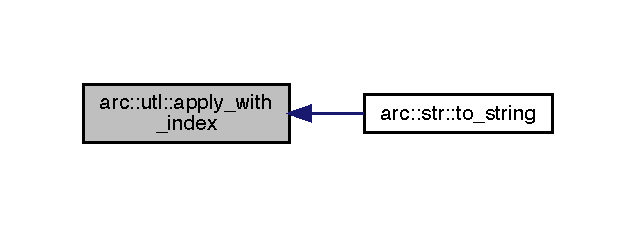
\includegraphics[width=305pt]{namespacearc_1_1utl_a77de5138bbfff1ea74f34f3018361186_icgraph}
\end{center}
\end{figure}
\mbox{\Hypertarget{namespacearc_1_1utl_a50e140f40e5a25a5fe253b94e6ab3403}\label{namespacearc_1_1utl_a50e140f40e5a25a5fe253b94e6ab3403}} 
\index{arc\+::utl@{arc\+::utl}!apply\+\_\+with\+\_\+index@{apply\+\_\+with\+\_\+index}}
\index{apply\+\_\+with\+\_\+index@{apply\+\_\+with\+\_\+index}!arc\+::utl@{arc\+::utl}}
\subsubsection{\texorpdfstring{apply\+\_\+with\+\_\+index()}{apply\_with\_index()}\hspace{0.1cm}{\footnotesize\ttfamily [3/6]}}
{\footnotesize\ttfamily template$<$typename C , typename T  = typename C\+::value\+\_\+type, typename I  = typename C\+::cont\+\_\+iterator, typename F $>$ \\
void arc\+::utl\+::apply\+\_\+with\+\_\+index (\begin{DoxyParamCaption}\item[{const C \&}]{cont\+\_\+,  }\item[{F}]{func\+\_\+ }\end{DoxyParamCaption})\hspace{0.3cm}{\ttfamily [inline]}, {\ttfamily [noexcept]}}

Apply a given functor to each element of a const container. Provide the current element index and the total number of elements.


\begin{DoxyTemplParams}{Template Parameters}
{\em C} & Type of container. \\
\hline
{\em T} & Type stored by C. \\
\hline
{\em I} & Type of const iterator of C. \\
\hline
{\em F} & Type of functor to be applied.\\
\hline
\end{DoxyTemplParams}

\begin{DoxyParams}{Parameters}
{\em cont\+\_\+} & Container to be applied to. \\
\hline
{\em func\+\_\+} & Functor to be applied. \\
\hline
\end{DoxyParams}
\mbox{\Hypertarget{namespacearc_1_1utl_ad77a0481ab72232b49349532b96f80fc}\label{namespacearc_1_1utl_ad77a0481ab72232b49349532b96f80fc}} 
\index{arc\+::utl@{arc\+::utl}!apply\+\_\+with\+\_\+index@{apply\+\_\+with\+\_\+index}}
\index{apply\+\_\+with\+\_\+index@{apply\+\_\+with\+\_\+index}!arc\+::utl@{arc\+::utl}}
\subsubsection{\texorpdfstring{apply\+\_\+with\+\_\+index()}{apply\_with\_index()}\hspace{0.1cm}{\footnotesize\ttfamily [4/6]}}
{\footnotesize\ttfamily template$<$typename A0 , typename A1 , typename F $>$ \\
void arc\+::utl\+::apply\+\_\+with\+\_\+index (\begin{DoxyParamCaption}\item[{const std\+::pair$<$ A0, A1 $>$ \&}]{pair\+\_\+,  }\item[{F}]{func\+\_\+ }\end{DoxyParamCaption})}

Call a functor on each element of a const pair. Provide the pair index and the total number of pair types.


\begin{DoxyTemplParams}{Template Parameters}
{\em A0} & First type stored by the pair. \\
\hline
{\em A1} & Second type stored by the pair. \\
\hline
{\em F} & Type of functor to be applied.\\
\hline
\end{DoxyTemplParams}

\begin{DoxyParams}{Parameters}
{\em pair\+\_\+} & Pair to be applied to. \\
\hline
{\em func\+\_\+} & Functor to be applied. \\
\hline
\end{DoxyParams}
\mbox{\Hypertarget{namespacearc_1_1utl_a2658c84859917c434ff3a7f667b21eca}\label{namespacearc_1_1utl_a2658c84859917c434ff3a7f667b21eca}} 
\index{arc\+::utl@{arc\+::utl}!apply\+\_\+with\+\_\+index@{apply\+\_\+with\+\_\+index}}
\index{apply\+\_\+with\+\_\+index@{apply\+\_\+with\+\_\+index}!arc\+::utl@{arc\+::utl}}
\subsubsection{\texorpdfstring{apply\+\_\+with\+\_\+index()}{apply\_with\_index()}\hspace{0.1cm}{\footnotesize\ttfamily [5/6]}}
{\footnotesize\ttfamily template$<$typename... A, typename F $>$ \\
void arc\+::utl\+::apply\+\_\+with\+\_\+index (\begin{DoxyParamCaption}\item[{std\+::tuple$<$ A... $>$ \&}]{tuple\+\_\+,  }\item[{F}]{func\+\_\+ }\end{DoxyParamCaption})}

Apply a given functor to each element of a tuple. Current tuple index and the total number of tuple types are provided.


\begin{DoxyTemplParams}{Template Parameters}
{\em A} & Types stored by the tuple. \\
\hline
{\em F} & Type of functor to be applied.\\
\hline
\end{DoxyTemplParams}

\begin{DoxyParams}{Parameters}
{\em tuple\+\_\+} & Tuple to be applied to. \\
\hline
{\em func\+\_\+} & Functor to be applied. \\
\hline
\end{DoxyParams}
Here is the call graph for this function\+:\nopagebreak
\begin{figure}[H]
\begin{center}
\leavevmode
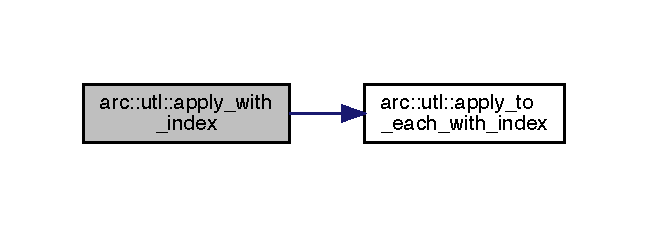
\includegraphics[width=311pt]{namespacearc_1_1utl_a2658c84859917c434ff3a7f667b21eca_cgraph}
\end{center}
\end{figure}
\mbox{\Hypertarget{namespacearc_1_1utl_ae57e12a4fd6beeb3a1a40bfd461c3a87}\label{namespacearc_1_1utl_ae57e12a4fd6beeb3a1a40bfd461c3a87}} 
\index{arc\+::utl@{arc\+::utl}!apply\+\_\+with\+\_\+index@{apply\+\_\+with\+\_\+index}}
\index{apply\+\_\+with\+\_\+index@{apply\+\_\+with\+\_\+index}!arc\+::utl@{arc\+::utl}}
\subsubsection{\texorpdfstring{apply\+\_\+with\+\_\+index()}{apply\_with\_index()}\hspace{0.1cm}{\footnotesize\ttfamily [6/6]}}
{\footnotesize\ttfamily template$<$typename... A, typename F $>$ \\
void arc\+::utl\+::apply\+\_\+with\+\_\+index (\begin{DoxyParamCaption}\item[{const std\+::tuple$<$ A... $>$ \&}]{tuple\+\_\+,  }\item[{F}]{func\+\_\+ }\end{DoxyParamCaption})}

Apply a given functor to each element of a const tuple. Current tuple index and the total number of tuple types are provided.


\begin{DoxyTemplParams}{Template Parameters}
{\em A} & Types stored by the tuple. \\
\hline
{\em F} & Type of functor to be applied.\\
\hline
\end{DoxyTemplParams}

\begin{DoxyParams}{Parameters}
{\em tuple\+\_\+} & Tuple to be applied to. \\
\hline
{\em func\+\_\+} & Functor to be applied. \\
\hline
\end{DoxyParams}
Here is the call graph for this function\+:\nopagebreak
\begin{figure}[H]
\begin{center}
\leavevmode
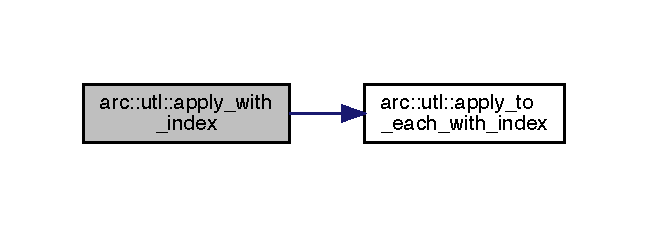
\includegraphics[width=311pt]{namespacearc_1_1utl_ae57e12a4fd6beeb3a1a40bfd461c3a87_cgraph}
\end{center}
\end{figure}

\chapter{Class Documentation}
\hypertarget{structarc_1_1str_1_1_tuple_to_string}{}\section{arc\+:\+:str\+:\+:Tuple\+To\+String Struct Reference}
\label{structarc_1_1str_1_1_tuple_to_string}\index{arc\+::str\+::\+Tuple\+To\+String@{arc\+::str\+::\+Tuple\+To\+String}}


{\ttfamily \#include $<$convert.\+hpp$>$}

\subsection*{Public Member Functions}
\begin{DoxyCompactItemize}
\item 
\mbox{\hyperlink{structarc_1_1str_1_1_tuple_to_string_ac2dac7554cf6813ef164c9ea01f3553a}{Tuple\+To\+String}} (std\+::stringstream \&stream\+\_\+, const std\+::string \&delim\+\_\+, const size\+\_\+t width\+\_\+)
\item 
{\footnotesize template$<$typename L $>$ }\\void \mbox{\hyperlink{structarc_1_1str_1_1_tuple_to_string_a91460084c852e91c61887015e0f91a7b}{operator()}} (const L \&val\+\_\+, const size\+\_\+t i\+\_\+, const size\+\_\+t)
\end{DoxyCompactItemize}
\subsection*{Private Attributes}
\begin{DoxyCompactItemize}
\item 
std\+::stringstream \& \mbox{\hyperlink{structarc_1_1str_1_1_tuple_to_string_adfa1e5289a45d5c1449694835b99fe68}{\+\_\+stream}}
\begin{DoxyCompactList}\small\item\em Stream to write to. \end{DoxyCompactList}\item 
const std\+::string \mbox{\hyperlink{structarc_1_1str_1_1_tuple_to_string_a822dbcaf492224fab6645ebf8dc7e5b1}{\+\_\+delim}}
\begin{DoxyCompactList}\small\item\em Delimiter added between elements. \end{DoxyCompactList}\item 
const size\+\_\+t \mbox{\hyperlink{structarc_1_1str_1_1_tuple_to_string_aa99def2d3e4827b56a2bc8a9e4b08e1e}{\+\_\+width}}
\begin{DoxyCompactList}\small\item\em Print width allocated to each element. \end{DoxyCompactList}\end{DoxyCompactItemize}


\subsection{Detailed Description}
Functor used by to\+\_\+string tuple method. Required while standard does not support template lambdas. Should be able to remove this in c++2a. 

\subsection{Constructor \& Destructor Documentation}
\mbox{\Hypertarget{structarc_1_1str_1_1_tuple_to_string_ac2dac7554cf6813ef164c9ea01f3553a}\label{structarc_1_1str_1_1_tuple_to_string_ac2dac7554cf6813ef164c9ea01f3553a}} 
\index{arc\+::str\+::\+Tuple\+To\+String@{arc\+::str\+::\+Tuple\+To\+String}!Tuple\+To\+String@{Tuple\+To\+String}}
\index{Tuple\+To\+String@{Tuple\+To\+String}!arc\+::str\+::\+Tuple\+To\+String@{arc\+::str\+::\+Tuple\+To\+String}}
\subsubsection{\texorpdfstring{Tuple\+To\+String()}{TupleToString()}}
{\footnotesize\ttfamily arc\+::str\+::\+Tuple\+To\+String\+::\+Tuple\+To\+String (\begin{DoxyParamCaption}\item[{std\+::stringstream \&}]{stream\+\_\+,  }\item[{const std\+::string \&}]{delim\+\_\+,  }\item[{const size\+\_\+t}]{width\+\_\+ }\end{DoxyParamCaption})\hspace{0.3cm}{\ttfamily [inline]}}

Construct a \mbox{\hyperlink{structarc_1_1str_1_1_tuple_to_string}{Tuple\+To\+String}} functor which will write to a given stream.


\begin{DoxyParams}{Parameters}
{\em stream\+\_\+} & Stream to write to. \\
\hline
{\em width\+\_\+} & Print width allocated to each element. \\
\hline
{\em delim\+\_\+} & Delimiter added between elements. \\
\hline
\end{DoxyParams}


\subsection{Member Function Documentation}
\mbox{\Hypertarget{structarc_1_1str_1_1_tuple_to_string_a91460084c852e91c61887015e0f91a7b}\label{structarc_1_1str_1_1_tuple_to_string_a91460084c852e91c61887015e0f91a7b}} 
\index{arc\+::str\+::\+Tuple\+To\+String@{arc\+::str\+::\+Tuple\+To\+String}!operator()@{operator()}}
\index{operator()@{operator()}!arc\+::str\+::\+Tuple\+To\+String@{arc\+::str\+::\+Tuple\+To\+String}}
\subsubsection{\texorpdfstring{operator()()}{operator()()}}
{\footnotesize\ttfamily template$<$typename L $>$ \\
void arc\+::str\+::\+Tuple\+To\+String\+::operator() (\begin{DoxyParamCaption}\item[{const L \&}]{val\+\_\+,  }\item[{const size\+\_\+t}]{i\+\_\+,  }\item[{const size\+\_\+t}]{ }\end{DoxyParamCaption})\hspace{0.3cm}{\ttfamily [inline]}}

Write the element to \+\_\+stream.


\begin{DoxyParams}{Parameters}
{\em val\+\_\+} & Value to write to the \+\_\+stream. \\
\hline
{\em i\+\_\+} & Index of element. \\
\hline
\end{DoxyParams}


\subsection{Member Data Documentation}
\mbox{\Hypertarget{structarc_1_1str_1_1_tuple_to_string_a822dbcaf492224fab6645ebf8dc7e5b1}\label{structarc_1_1str_1_1_tuple_to_string_a822dbcaf492224fab6645ebf8dc7e5b1}} 
\index{arc\+::str\+::\+Tuple\+To\+String@{arc\+::str\+::\+Tuple\+To\+String}!\+\_\+delim@{\+\_\+delim}}
\index{\+\_\+delim@{\+\_\+delim}!arc\+::str\+::\+Tuple\+To\+String@{arc\+::str\+::\+Tuple\+To\+String}}
\subsubsection{\texorpdfstring{\+\_\+delim}{\_delim}}
{\footnotesize\ttfamily const std\+::string arc\+::str\+::\+Tuple\+To\+String\+::\+\_\+delim\hspace{0.3cm}{\ttfamily [private]}}



Delimiter added between elements. 

\mbox{\Hypertarget{structarc_1_1str_1_1_tuple_to_string_adfa1e5289a45d5c1449694835b99fe68}\label{structarc_1_1str_1_1_tuple_to_string_adfa1e5289a45d5c1449694835b99fe68}} 
\index{arc\+::str\+::\+Tuple\+To\+String@{arc\+::str\+::\+Tuple\+To\+String}!\+\_\+stream@{\+\_\+stream}}
\index{\+\_\+stream@{\+\_\+stream}!arc\+::str\+::\+Tuple\+To\+String@{arc\+::str\+::\+Tuple\+To\+String}}
\subsubsection{\texorpdfstring{\+\_\+stream}{\_stream}}
{\footnotesize\ttfamily std\+::stringstream\& arc\+::str\+::\+Tuple\+To\+String\+::\+\_\+stream\hspace{0.3cm}{\ttfamily [private]}}



Stream to write to. 

\mbox{\Hypertarget{structarc_1_1str_1_1_tuple_to_string_aa99def2d3e4827b56a2bc8a9e4b08e1e}\label{structarc_1_1str_1_1_tuple_to_string_aa99def2d3e4827b56a2bc8a9e4b08e1e}} 
\index{arc\+::str\+::\+Tuple\+To\+String@{arc\+::str\+::\+Tuple\+To\+String}!\+\_\+width@{\+\_\+width}}
\index{\+\_\+width@{\+\_\+width}!arc\+::str\+::\+Tuple\+To\+String@{arc\+::str\+::\+Tuple\+To\+String}}
\subsubsection{\texorpdfstring{\+\_\+width}{\_width}}
{\footnotesize\ttfamily const size\+\_\+t arc\+::str\+::\+Tuple\+To\+String\+::\+\_\+width\hspace{0.3cm}{\ttfamily [private]}}



Print width allocated to each element. 



The documentation for this struct was generated from the following file\+:\begin{DoxyCompactItemize}
\item 
include/arctk/str/\mbox{\hyperlink{convert_8hpp}{convert.\+hpp}}\end{DoxyCompactItemize}

\chapter{File Documentation}
\hypertarget{config_8hpp}{}\section{include/arctk/config.hpp File Reference}
\label{config_8hpp}\index{include/arctk/config.\+hpp@{include/arctk/config.\+hpp}}
{\ttfamily \#include $<$cstdint$>$}\newline
Include dependency graph for config.\+hpp\+:\nopagebreak
\begin{figure}[H]
\begin{center}
\leavevmode
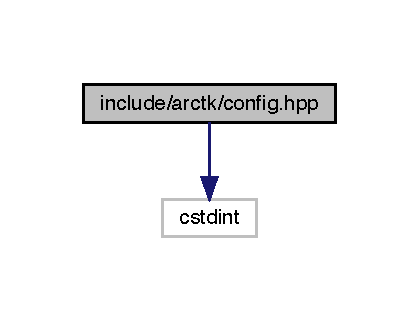
\includegraphics[width=201pt]{config_8hpp__incl}
\end{center}
\end{figure}
This graph shows which files directly or indirectly include this file\+:\nopagebreak
\begin{figure}[H]
\begin{center}
\leavevmode
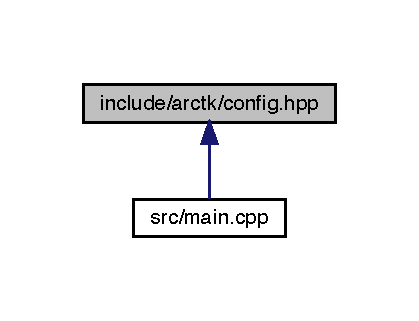
\includegraphics[width=201pt]{config_8hpp__dep__incl}
\end{center}
\end{figure}
\subsection*{Namespaces}
\begin{DoxyCompactItemize}
\item 
 \mbox{\hyperlink{namespacearc}{arc}}
\begin{DoxyCompactList}\small\item\em arctk namespace \end{DoxyCompactList}\item 
 \mbox{\hyperlink{namespacearc_1_1config}{arc\+::config}}
\begin{DoxyCompactList}\small\item\em configuration namespace \end{DoxyCompactList}\end{DoxyCompactItemize}
\subsection*{Variables}
\begin{DoxyCompactItemize}
\item 
constexpr const uint64\+\_\+t \mbox{\hyperlink{namespacearc_1_1config_a2d17637229eb1a5c1cd130d0945a5308}{arc\+::config\+::\+V\+E\+R\+S\+I\+O\+N\+\_\+\+M\+A\+J\+OR}} = 0
\begin{DoxyCompactList}\small\item\em Version major number. \end{DoxyCompactList}\item 
constexpr const uint64\+\_\+t \mbox{\hyperlink{namespacearc_1_1config_ad647132a40a28b2241f0406b168c1874}{arc\+::config\+::\+V\+E\+R\+S\+I\+O\+N\+\_\+\+M\+I\+N\+OR}} = 0
\begin{DoxyCompactList}\small\item\em Version minor number. \end{DoxyCompactList}\item 
constexpr const uint64\+\_\+t \mbox{\hyperlink{namespacearc_1_1config_afc8283f15f7b5502fe48b6616a5d1207}{arc\+::config\+::\+V\+E\+R\+S\+I\+O\+N\+\_\+\+P\+A\+T\+CH}} = 1168
\begin{DoxyCompactList}\small\item\em Version patch number. \end{DoxyCompactList}\item 
constexpr const char $\ast$ \mbox{\hyperlink{namespacearc_1_1config_a07a575e6c44170c6f629402c89f0a044}{arc\+::config\+::\+D\+IR}} = \char`\"{}/Users/freddy/arctk\char`\"{}
\begin{DoxyCompactList}\small\item\em Build directory. \end{DoxyCompactList}\item 
constexpr const char $\ast$ \mbox{\hyperlink{namespacearc_1_1config_ad3826980a7fae51393802afb8fdcc382}{arc\+::config\+::\+B\+R\+A\+N\+CH}} = \char`\"{}master\char`\"{}
\begin{DoxyCompactList}\small\item\em Build branch. \end{DoxyCompactList}\item 
constexpr const char $\ast$ \mbox{\hyperlink{namespacearc_1_1config_acba74c1165508123cf039684296dd007}{arc\+::config\+::\+H\+A\+SH}} = \char`\"{}f23a0bb\char`\"{}
\begin{DoxyCompactList}\small\item\em Git hash. \end{DoxyCompactList}\item 
constexpr const char $\ast$ \mbox{\hyperlink{namespacearc_1_1config_abfeebd457f762473ba01e07e14c8d084}{arc\+::config\+::\+C\+O\+M\+P\+I\+L\+ER}} = \char`\"{}Clang\char`\"{}
\begin{DoxyCompactList}\small\item\em Compiler id. \end{DoxyCompactList}\item 
constexpr const char $\ast$ \mbox{\hyperlink{namespacearc_1_1config_ad6eeea3db680c98dc954b7951924fb0b}{arc\+::config\+::\+T\+Y\+PE}} = \char`\"{}debug\char`\"{}
\begin{DoxyCompactList}\small\item\em Optimisation type. \end{DoxyCompactList}\item 
constexpr const char $\ast$ \mbox{\hyperlink{namespacearc_1_1config_aa60520859e13bbee2fb47d352d337c87}{arc\+::config\+::\+D\+A\+TE}} = \char`\"{}2018-\/05-\/30\char`\"{}
\begin{DoxyCompactList}\small\item\em Build date. \end{DoxyCompactList}\item 
constexpr const char $\ast$ \mbox{\hyperlink{namespacearc_1_1config_a91b9e1afbcd188b61eb1430caeac30db}{arc\+::config\+::\+M\+O\+D\+\_\+\+C\+O\+RE}} = \char`\"{}true\char`\"{}
\begin{DoxyCompactList}\small\item\em Arctk core module status. \end{DoxyCompactList}\end{DoxyCompactItemize}


\subsection{Detailed Description}
\begin{DoxyDate}{Date}
15/05/2018 
\end{DoxyDate}
\begin{DoxyAuthor}{Author}
Freddy Wordingham
\end{DoxyAuthor}
Library build-\/time configuration constants. 
\hypertarget{constant_8hpp}{}\section{include/arctk/constant.hpp File Reference}
\label{constant_8hpp}\index{include/arctk/constant.\+hpp@{include/arctk/constant.\+hpp}}
{\ttfamily \#include $<$arctk/constant/math.\+hpp$>$}\newline
{\ttfamily \#include $<$arctk/constant/phys.\+hpp$>$}\newline
Include dependency graph for constant.\+hpp\+:\nopagebreak
\begin{figure}[H]
\begin{center}
\leavevmode
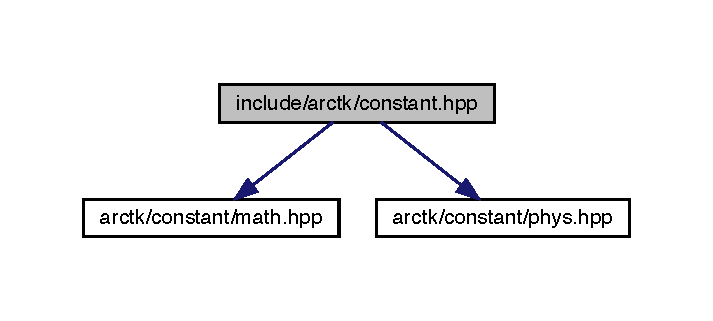
\includegraphics[width=342pt]{constant_8hpp__incl}
\end{center}
\end{figure}
This graph shows which files directly or indirectly include this file\+:\nopagebreak
\begin{figure}[H]
\begin{center}
\leavevmode
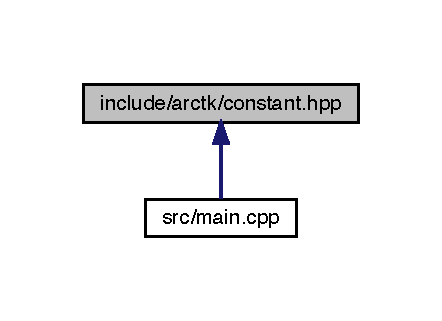
\includegraphics[width=212pt]{constant_8hpp__dep__incl}
\end{center}
\end{figure}


\subsection{Detailed Description}
\begin{DoxyDate}{Date}
29/05/2018 
\end{DoxyDate}
\begin{DoxyAuthor}{Author}
Freddy Wordingham
\end{DoxyAuthor}
Collection of constants. 
\hypertarget{math_8hpp}{}\section{include/arctk/constant/math.hpp File Reference}
\label{math_8hpp}\index{include/arctk/constant/math.\+hpp@{include/arctk/constant/math.\+hpp}}
This graph shows which files directly or indirectly include this file\+:\nopagebreak
\begin{figure}[H]
\begin{center}
\leavevmode
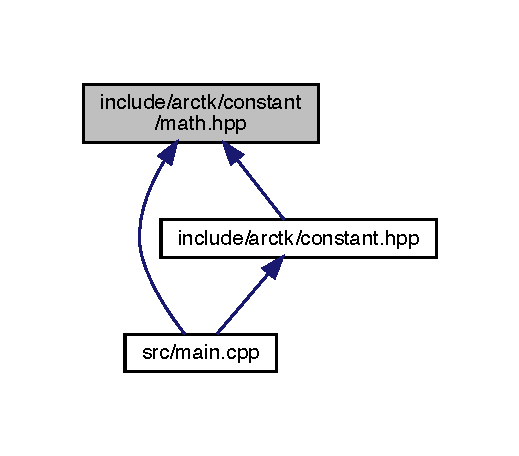
\includegraphics[width=249pt]{math_8hpp__dep__incl}
\end{center}
\end{figure}
\subsection*{Namespaces}
\begin{DoxyCompactItemize}
\item 
 \mbox{\hyperlink{namespacearc}{arc}}
\begin{DoxyCompactList}\small\item\em arctk namespace \end{DoxyCompactList}\item 
 \mbox{\hyperlink{namespacearc_1_1constant}{arc\+::constant}}
\begin{DoxyCompactList}\small\item\em constants namespace \end{DoxyCompactList}\end{DoxyCompactItemize}
\subsection*{Variables}
\begin{DoxyCompactItemize}
\item 
constexpr const double \mbox{\hyperlink{namespacearc_1_1constant_a3eccb0dc76feae32072ab77709824a47}{arc\+::constant\+::\+PI}} = 3.\+141592653589793238462643383279502884197169399375105820974
\begin{DoxyCompactList}\small\item\em Archimedes\textquotesingle{} Constant. \end{DoxyCompactList}\item 
constexpr const double \mbox{\hyperlink{namespacearc_1_1constant_a9db9629d8a4236d7f102c667695b31cb}{arc\+::constant\+::\+E\+XP}} = 2.\+718281828459045235360287471352662497757247093699959574966
\begin{DoxyCompactList}\small\item\em Euler\textquotesingle{}s Number. \end{DoxyCompactList}\end{DoxyCompactItemize}


\subsection{Detailed Description}
\begin{DoxyDate}{Date}
30/05/2018 
\end{DoxyDate}
\begin{DoxyAuthor}{Author}
Freddy Wordingham
\end{DoxyAuthor}
Mathematical constants. 
\hypertarget{phys_8hpp}{}\section{include/arctk/constant/phys.hpp File Reference}
\label{phys_8hpp}\index{include/arctk/constant/phys.\+hpp@{include/arctk/constant/phys.\+hpp}}
This graph shows which files directly or indirectly include this file\+:\nopagebreak
\begin{figure}[H]
\begin{center}
\leavevmode
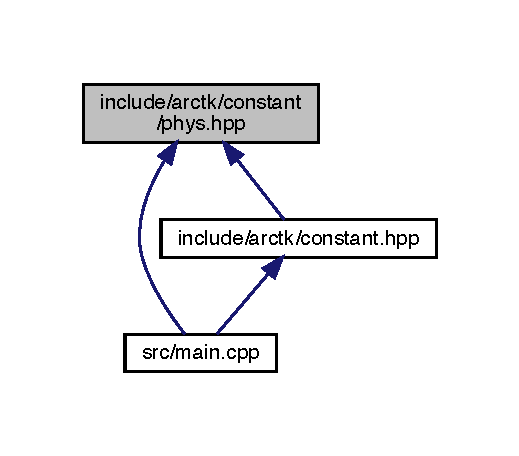
\includegraphics[width=249pt]{phys_8hpp__dep__incl}
\end{center}
\end{figure}
\subsection*{Namespaces}
\begin{DoxyCompactItemize}
\item 
 \mbox{\hyperlink{namespacearc}{arc}}
\begin{DoxyCompactList}\small\item\em arctk namespace \end{DoxyCompactList}\item 
 \mbox{\hyperlink{namespacearc_1_1constant}{arc\+::constant}}
\begin{DoxyCompactList}\small\item\em constants namespace \end{DoxyCompactList}\end{DoxyCompactItemize}
\subsection*{Variables}
\begin{DoxyCompactItemize}
\item 
constexpr const double \mbox{\hyperlink{namespacearc_1_1constant_a7380a245f82a0bc10f7cc9b7140d4e14}{arc\+::constant\+::\+S\+P\+E\+E\+D\+\_\+\+O\+F\+\_\+\+L\+I\+G\+HT}} = 2.\+99792458e+8
\begin{DoxyCompactList}\small\item\em Speed of light in vacuum. \end{DoxyCompactList}\end{DoxyCompactItemize}


\subsection{Detailed Description}
\begin{DoxyDate}{Date}
30/05/2018 
\end{DoxyDate}
\begin{DoxyAuthor}{Author}
Freddy Wordingham
\end{DoxyAuthor}
Physical constants. 
\hypertarget{format_8hpp}{}\section{include/arctk/format.hpp File Reference}
\label{format_8hpp}\index{include/arctk/format.\+hpp@{include/arctk/format.\+hpp}}
{\ttfamily \#include $<$arctk/format/table.\+hpp$>$}\newline
Include dependency graph for format.\+hpp\+:\nopagebreak
\begin{figure}[H]
\begin{center}
\leavevmode
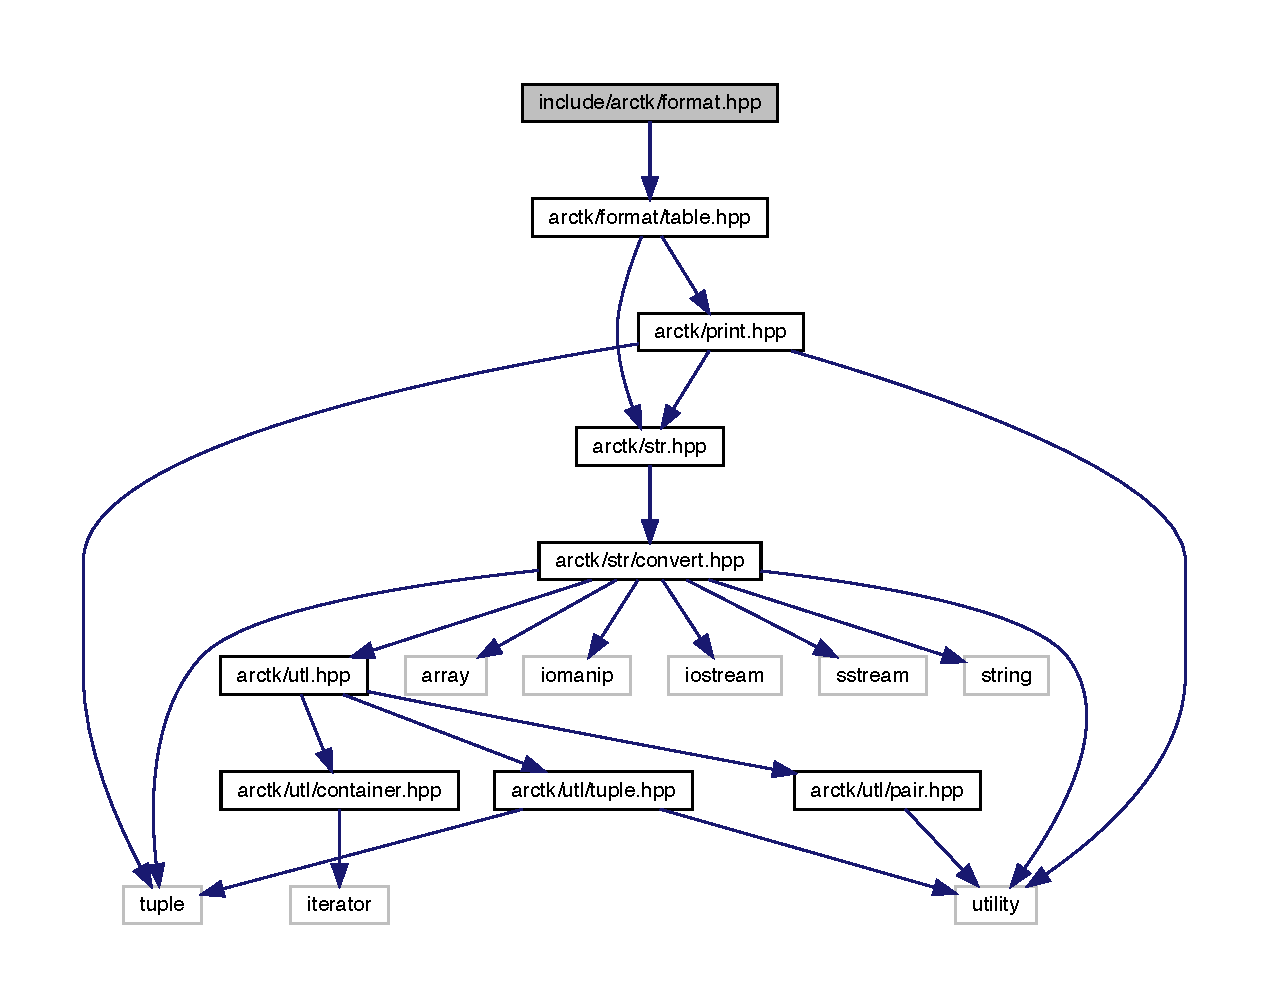
\includegraphics[width=350pt]{format_8hpp__incl}
\end{center}
\end{figure}
This graph shows which files directly or indirectly include this file\+:\nopagebreak
\begin{figure}[H]
\begin{center}
\leavevmode
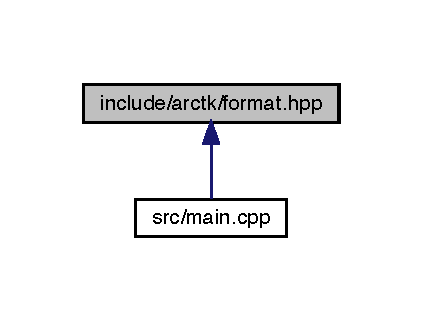
\includegraphics[width=203pt]{format_8hpp__dep__incl}
\end{center}
\end{figure}


\subsection{Detailed Description}
\begin{DoxyDate}{Date}
28/05/2018 
\end{DoxyDate}
\begin{DoxyAuthor}{Author}
Freddy Wordingham
\end{DoxyAuthor}
Collection of format functions. 
\hypertarget{table_8hpp}{}\section{include/arctk/format/table.hpp File Reference}
\label{table_8hpp}\index{include/arctk/format/table.\+hpp@{include/arctk/format/table.\+hpp}}
{\ttfamily \#include $<$arctk/print.\+hpp$>$}\newline
{\ttfamily \#include $<$arctk/str.\+hpp$>$}\newline
Include dependency graph for table.\+hpp\+:\nopagebreak
\begin{figure}[H]
\begin{center}
\leavevmode
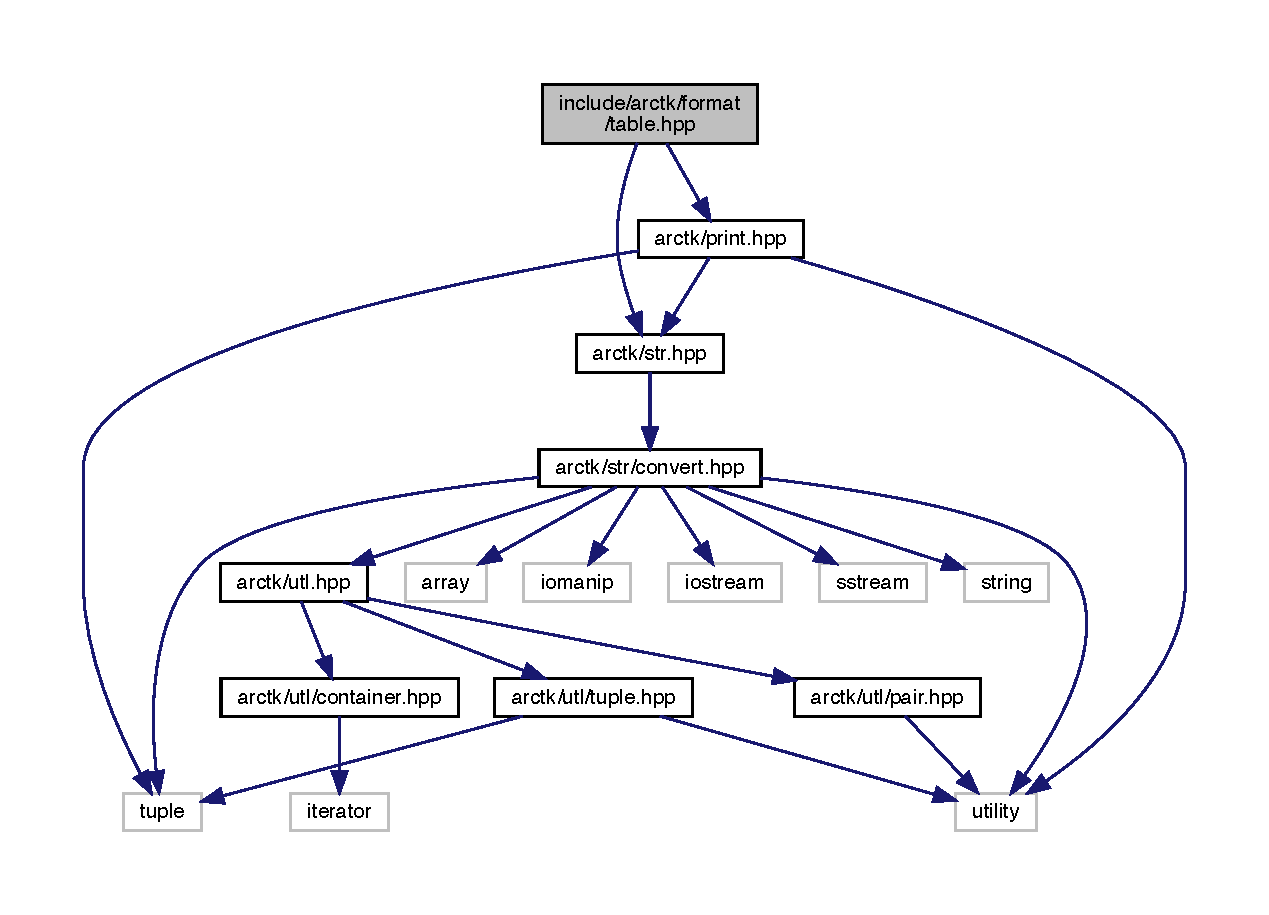
\includegraphics[width=350pt]{table_8hpp__incl}
\end{center}
\end{figure}
This graph shows which files directly or indirectly include this file\+:\nopagebreak
\begin{figure}[H]
\begin{center}
\leavevmode
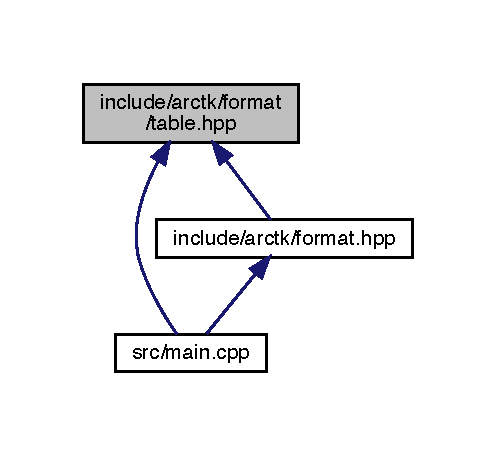
\includegraphics[width=238pt]{table_8hpp__dep__incl}
\end{center}
\end{figure}
\subsection*{Namespaces}
\begin{DoxyCompactItemize}
\item 
 \mbox{\hyperlink{namespacearc}{arc}}
\begin{DoxyCompactList}\small\item\em arctk namespace \end{DoxyCompactList}\item 
 \mbox{\hyperlink{namespacearc_1_1format}{arc\+::format}}
\begin{DoxyCompactList}\small\item\em format namespace \end{DoxyCompactList}\end{DoxyCompactItemize}
\subsection*{Functions}
\begin{DoxyCompactItemize}
\item 
{\footnotesize template$<$typename C , typename T  = typename C\+::value\+\_\+type, typename I  = typename C\+::const\+\_\+iterator$>$ }\\std\+::string \mbox{\hyperlink{namespacearc_1_1format_a0c2871882ac6679e40c71a2176ddd529}{arc\+::format\+::table}} (const C \&cont\+\_\+, size\+\_\+t width\+\_\+=0, const std\+::string \&delim\+\_\+=\char`\"{}, \char`\"{}) noexcept
\end{DoxyCompactItemize}


\subsection{Detailed Description}
\begin{DoxyDate}{Date}
28/05/2018 
\end{DoxyDate}
\begin{DoxyAuthor}{Author}
Freddy Wordingham
\end{DoxyAuthor}
Table formating functions. 
\hypertarget{print_8hpp}{}\section{include/arctk/print.hpp File Reference}
\label{print_8hpp}\index{include/arctk/print.\+hpp@{include/arctk/print.\+hpp}}
{\ttfamily \#include $<$tuple$>$}\newline
{\ttfamily \#include $<$utility$>$}\newline
{\ttfamily \#include $<$arctk/str.\+hpp$>$}\newline
Include dependency graph for print.\+hpp\+:\nopagebreak
\begin{figure}[H]
\begin{center}
\leavevmode
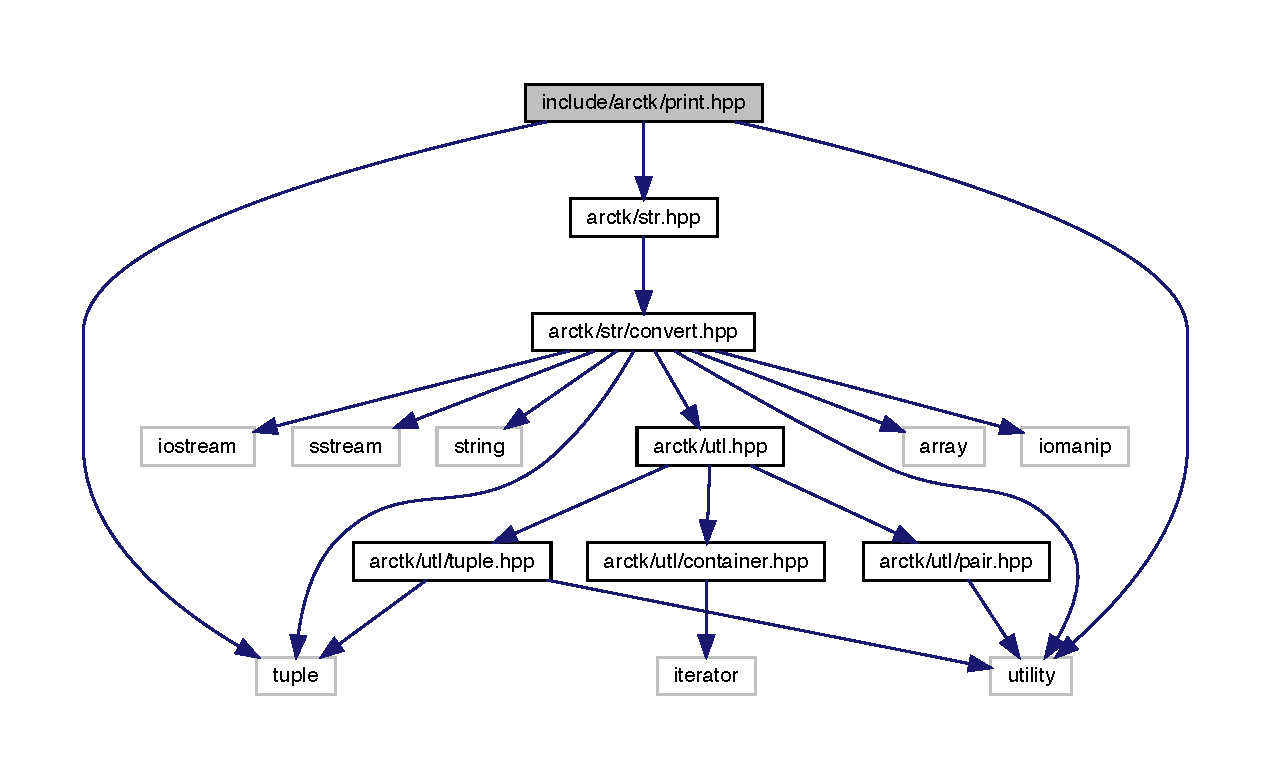
\includegraphics[width=350pt]{print_8hpp__incl}
\end{center}
\end{figure}
This graph shows which files directly or indirectly include this file\+:\nopagebreak
\begin{figure}[H]
\begin{center}
\leavevmode
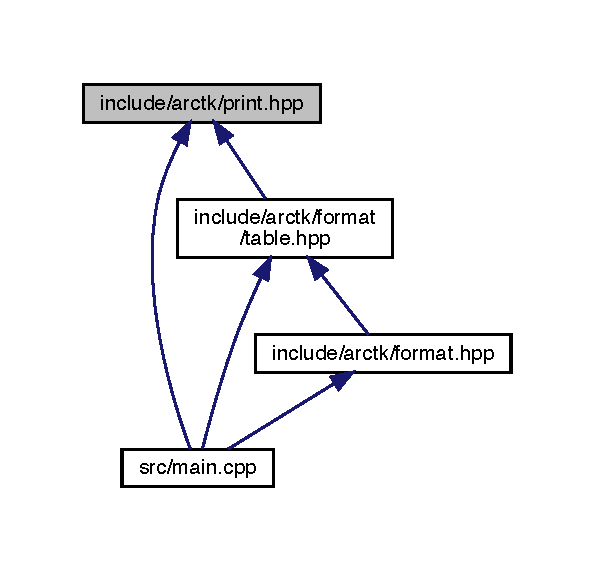
\includegraphics[width=285pt]{print_8hpp__dep__incl}
\end{center}
\end{figure}
\subsection*{Namespaces}
\begin{DoxyCompactItemize}
\item 
 \mbox{\hyperlink{namespacearc}{arc}}
\begin{DoxyCompactList}\small\item\em arctk namespace \end{DoxyCompactList}\end{DoxyCompactItemize}
\subsection*{Functions}
\begin{DoxyCompactItemize}
\item 
{\footnotesize template$<$typename S , typename C , typename T  = typename C\+::value\+\_\+type, typename I  = typename C\+::const\+\_\+iterator, typename  = typename std\+::enable\+\_\+if$<$!std\+::is\+\_\+same$<$\+C, std\+::string$>$\+::value$>$\+::type$>$ }\\S \& \mbox{\hyperlink{namespacearc_af1dbfe8cd5fb9a3a09bfe75114f9057b}{arc\+::operator$<$$<$}} (S \&stream\+\_\+, const C \&cont\+\_\+)
\item 
{\footnotesize template$<$typename S , typename A0 , typename A1 $>$ }\\S \& \mbox{\hyperlink{namespacearc_ae2d7de3bec14ccfaf44ea00f134895f9}{arc\+::operator$<$$<$}} (S \&stream\+\_\+, const std\+::pair$<$ A0, A1 $>$ \&pair\+\_\+)
\item 
{\footnotesize template$<$typename S , typename... A$>$ }\\S \& \mbox{\hyperlink{namespacearc_a50e1f816ae8c0b1a32e9adabbe66579a}{arc\+::operator$<$$<$}} (S \&stream\+\_\+, const std\+::tuple$<$ A... $>$ \&tup\+\_\+)
\end{DoxyCompactItemize}


\subsection{Detailed Description}
\begin{DoxyDate}{Date}
28/05/2018 
\end{DoxyDate}
\begin{DoxyAuthor}{Author}
Freddy Wordingham
\end{DoxyAuthor}
Collection of print functions. 
\hypertarget{prop_2container_8hpp}{}\section{include/arctk/prop/container.hpp File Reference}
\label{prop_2container_8hpp}\index{include/arctk/prop/container.\+hpp@{include/arctk/prop/container.\+hpp}}
{\ttfamily \#include $<$algorithm$>$}\newline
{\ttfamily \#include $<$cassert$>$}\newline
{\ttfamily \#include $<$iterator$>$}\newline
Include dependency graph for container.\+hpp\+:\nopagebreak
\begin{figure}[H]
\begin{center}
\leavevmode
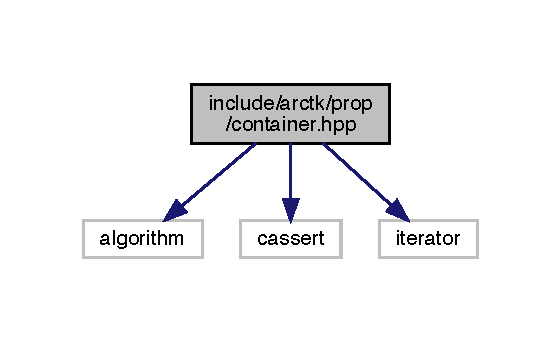
\includegraphics[width=269pt]{prop_2container_8hpp__incl}
\end{center}
\end{figure}
This graph shows which files directly or indirectly include this file\+:\nopagebreak
\begin{figure}[H]
\begin{center}
\leavevmode
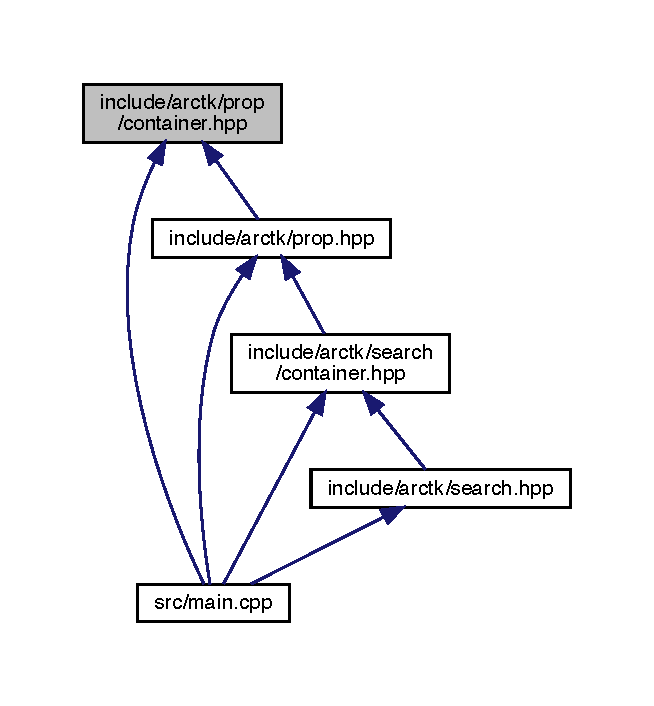
\includegraphics[width=314pt]{prop_2container_8hpp__dep__incl}
\end{center}
\end{figure}
\subsection*{Namespaces}
\begin{DoxyCompactItemize}
\item 
 \mbox{\hyperlink{namespacearc}{arc}}
\begin{DoxyCompactList}\small\item\em arctk namespace \end{DoxyCompactList}\item 
 \mbox{\hyperlink{namespacearc_1_1prop}{arc\+::prop}}
\begin{DoxyCompactList}\small\item\em properties namespace \end{DoxyCompactList}\end{DoxyCompactItemize}
\subsection*{Functions}
\begin{DoxyCompactItemize}
\item 
{\footnotesize template$<$typename C , typename T  = typename C\+::value\+\_\+type, typename I  = typename C\+::const\+\_\+iterator$>$ }\\bool \mbox{\hyperlink{namespacearc_1_1prop_a54974d0d56ee90909eac6cdd1b94cff5}{arc\+::prop\+::contains}} (const C \&cont\+\_\+, const T \&val\+\_\+) noexcept
\item 
{\footnotesize template$<$typename C , typename T  = typename C\+::value\+\_\+type, typename I  = typename C\+::const\+\_\+iterator$>$ }\\bool \mbox{\hyperlink{namespacearc_1_1prop_a026d439c76bdafd78b68875044d7b087}{arc\+::prop\+::ascending}} (const C \&cont\+\_\+) noexcept
\item 
{\footnotesize template$<$typename C , typename T  = typename C\+::value\+\_\+type, typename I  = typename C\+::const\+\_\+iterator$>$ }\\bool \mbox{\hyperlink{namespacearc_1_1prop_a156186f9684c79f4f28bb793af35f0bd}{arc\+::prop\+::descending}} (const C \&cont\+\_\+) noexcept
\item 
{\footnotesize template$<$typename C , typename T  = typename C\+::value\+\_\+type, typename I  = typename C\+::const\+\_\+iterator$>$ }\\bool \mbox{\hyperlink{namespacearc_1_1prop_a0b6cfeae4fa16eddbb6b7f1e9c355258}{arc\+::prop\+::monotonic}} (const C \&cont\+\_\+) noexcept
\item 
{\footnotesize template$<$typename C , typename T  = typename C\+::value\+\_\+type, typename I  = typename C\+::const\+\_\+iterator$>$ }\\bool \mbox{\hyperlink{namespacearc_1_1prop_aa5ffd8e519bbfe13d8b6c9b9ebf81855}{arc\+::prop\+::uniform}} (const C \&cont\+\_\+) noexcept
\item 
{\footnotesize template$<$typename C , typename T  = typename C\+::value\+\_\+type, typename I  = typename C\+::const\+\_\+iterator$>$ }\\bool \mbox{\hyperlink{namespacearc_1_1prop_a160eaff41b7223c20c03ca76ee4e1fb9}{arc\+::prop\+::within}} (const C \&cont\+\_\+, const T \&val\+\_\+) noexcept
\item 
{\footnotesize template$<$typename C , typename T  = typename C\+::value\+\_\+type, typename I  = typename C\+::const\+\_\+iterator$>$ }\\bool \mbox{\hyperlink{namespacearc_1_1prop_a965c4011bd27be186a9b63d69f27c4e4}{arc\+::prop\+::always\+\_\+less\+\_\+than}} (const C \&cont\+\_\+, const T \&limit\+\_\+) noexcept
\item 
{\footnotesize template$<$typename C , typename T  = typename C\+::value\+\_\+type, typename I  = typename C\+::const\+\_\+iterator$>$ }\\bool \mbox{\hyperlink{namespacearc_1_1prop_aa5ade88a045bf078e0dffe0418f133d5}{arc\+::prop\+::always\+\_\+less\+\_\+than\+\_\+or\+\_\+equal\+\_\+to}} (const C \&cont\+\_\+, const T \&limit\+\_\+) noexcept
\item 
{\footnotesize template$<$typename C , typename T  = typename C\+::value\+\_\+type, typename I  = typename C\+::const\+\_\+iterator$>$ }\\bool \mbox{\hyperlink{namespacearc_1_1prop_a0786e461abacc64a0479a9c29cebcfa9}{arc\+::prop\+::always\+\_\+greater\+\_\+than}} (const C \&cont\+\_\+, const T \&limit\+\_\+) noexcept
\item 
{\footnotesize template$<$typename C , typename T  = typename C\+::value\+\_\+type, typename I  = typename C\+::const\+\_\+iterator$>$ }\\bool \mbox{\hyperlink{namespacearc_1_1prop_a858cf86c6dc1c5ad0a337ac8adc7a787}{arc\+::prop\+::always\+\_\+greater\+\_\+than\+\_\+or\+\_\+equal\+\_\+to}} (const C \&cont\+\_\+, const T \&limit\+\_\+) noexcept
\end{DoxyCompactItemize}


\subsection{Detailed Description}
\begin{DoxyDate}{Date}
29/05/2018 
\end{DoxyDate}
\begin{DoxyAuthor}{Author}
Freddy Wordingham
\end{DoxyAuthor}
Container proprty functions. 
\hypertarget{search_2container_8hpp}{}\section{include/arctk/search/container.hpp File Reference}
\label{search_2container_8hpp}\index{include/arctk/search/container.\+hpp@{include/arctk/search/container.\+hpp}}
{\ttfamily \#include $<$cassert$>$}\newline
{\ttfamily \#include $<$iterator$>$}\newline
{\ttfamily \#include $<$arctk/prop.\+hpp$>$}\newline
Include dependency graph for container.\+hpp\+:\nopagebreak
\begin{figure}[H]
\begin{center}
\leavevmode
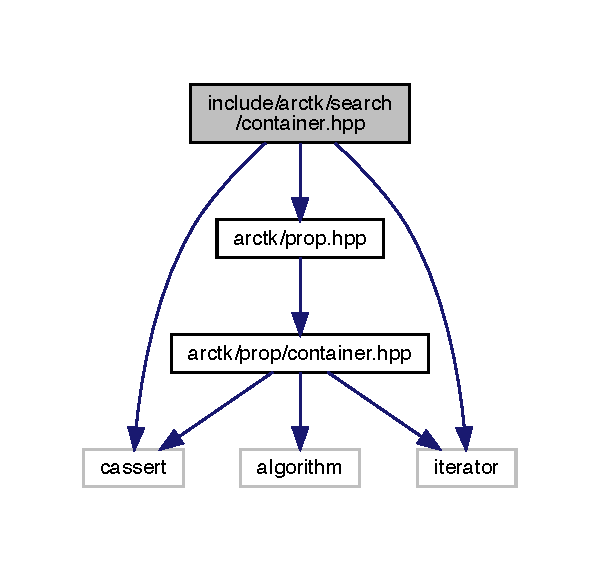
\includegraphics[width=288pt]{search_2container_8hpp__incl}
\end{center}
\end{figure}
This graph shows which files directly or indirectly include this file\+:\nopagebreak
\begin{figure}[H]
\begin{center}
\leavevmode
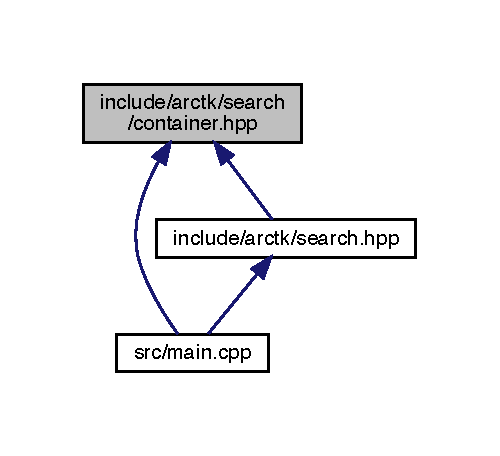
\includegraphics[width=240pt]{search_2container_8hpp__dep__incl}
\end{center}
\end{figure}
\subsection*{Namespaces}
\begin{DoxyCompactItemize}
\item 
 \mbox{\hyperlink{namespacearc}{arc}}
\begin{DoxyCompactList}\small\item\em arctk namespace \end{DoxyCompactList}\item 
 \mbox{\hyperlink{namespacearc_1_1search}{arc\+::search}}
\begin{DoxyCompactList}\small\item\em search namespace \end{DoxyCompactList}\end{DoxyCompactItemize}
\subsection*{Functions}
\begin{DoxyCompactItemize}
\item 
{\footnotesize template$<$typename C , typename T  = typename C\+::value\+\_\+type, typename I  = typename C\+::const\+\_\+iterator$>$ }\\size\+\_\+t \mbox{\hyperlink{namespacearc_1_1search_ae457da2cc210e1edfaf811bc83154f4b}{arc\+::search\+::min\+\_\+index}} (const C \&cont\+\_\+) noexcept
\item 
{\footnotesize template$<$typename C , typename T  = typename C\+::value\+\_\+type, typename I  = typename C\+::const\+\_\+iterator$>$ }\\size\+\_\+t \mbox{\hyperlink{namespacearc_1_1search_aac33af22b716309501eaa7f5a10cc1d0}{arc\+::search\+::max\+\_\+index}} (const C \&cont\+\_\+) noexcept
\item 
{\footnotesize template$<$typename C , typename T  = typename C\+::value\+\_\+type, typename I  = typename C\+::const\+\_\+iterator$>$ }\\T \mbox{\hyperlink{namespacearc_1_1search_a1cf0173ae1f8475d3b1652c006d5649d}{arc\+::search\+::min}} (const C \&cont\+\_\+) noexcept
\item 
{\footnotesize template$<$typename C , typename T  = typename C\+::value\+\_\+type, typename I  = typename C\+::const\+\_\+iterator$>$ }\\T \mbox{\hyperlink{namespacearc_1_1search_ab5608d27962c637137d2c243213fa366}{arc\+::search\+::max}} (const C \&cont\+\_\+) noexcept
\item 
{\footnotesize template$<$typename C , typename T  = typename C\+::value\+\_\+type, typename I  = typename C\+::const\+\_\+iterator$>$ }\\size\+\_\+t \mbox{\hyperlink{namespacearc_1_1search_ab5171637f0c917d6f387cb619a319ab5}{arc\+::search\+::lower}} (const C \&cont\+\_\+, const T \&val\+\_\+) noexcept
\item 
{\footnotesize template$<$typename C , typename T  = typename C\+::value\+\_\+type, typename I  = typename C\+::const\+\_\+iterator$>$ }\\size\+\_\+t \mbox{\hyperlink{namespacearc_1_1search_a66f5d701ff409cb5e2673a4d5864cd11}{arc\+::search\+::upper}} (const C \&cont\+\_\+, const T \&val\+\_\+) noexcept
\end{DoxyCompactItemize}


\subsection{Detailed Description}
\begin{DoxyDate}{Date}
29/05/2018 
\end{DoxyDate}
\begin{DoxyAuthor}{Author}
Freddy Wordingham
\end{DoxyAuthor}
Container search functions. 
\hypertarget{utl_2container_8hpp}{}\section{include/arctk/utl/container.hpp File Reference}
\label{utl_2container_8hpp}\index{include/arctk/utl/container.\+hpp@{include/arctk/utl/container.\+hpp}}
{\ttfamily \#include $<$iterator$>$}\newline
Include dependency graph for container.\+hpp\+:\nopagebreak
\begin{figure}[H]
\begin{center}
\leavevmode
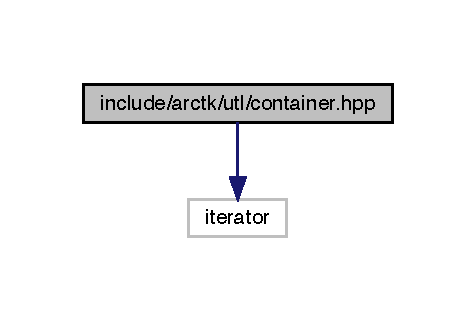
\includegraphics[width=228pt]{utl_2container_8hpp__incl}
\end{center}
\end{figure}
This graph shows which files directly or indirectly include this file\+:\nopagebreak
\begin{figure}[H]
\begin{center}
\leavevmode
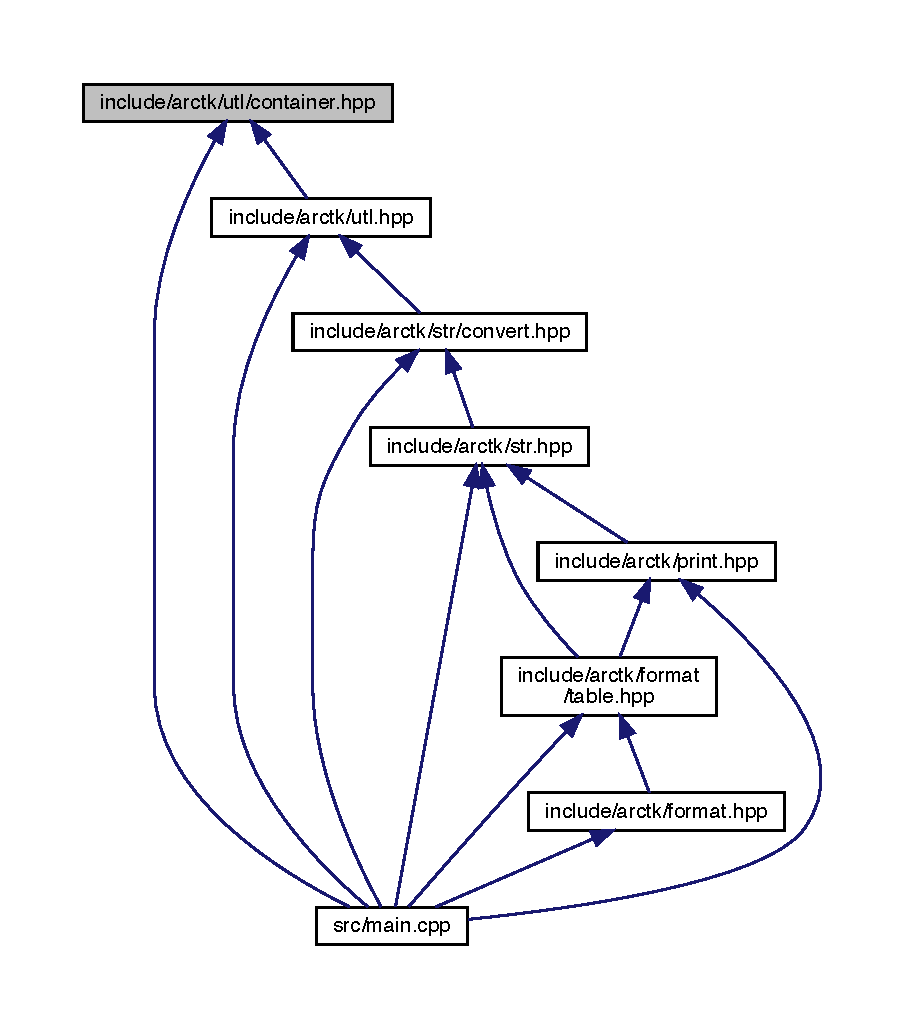
\includegraphics[width=350pt]{utl_2container_8hpp__dep__incl}
\end{center}
\end{figure}
\subsection*{Namespaces}
\begin{DoxyCompactItemize}
\item 
 \mbox{\hyperlink{namespacearc}{arc}}
\begin{DoxyCompactList}\small\item\em arctk namespace \end{DoxyCompactList}\item 
 \mbox{\hyperlink{namespacearc_1_1utl}{arc\+::utl}}
\begin{DoxyCompactList}\small\item\em utility namespace \end{DoxyCompactList}\end{DoxyCompactItemize}
\subsection*{Functions}
\begin{DoxyCompactItemize}
\item 
{\footnotesize template$<$typename C , typename T  = typename C\+::value\+\_\+type, typename I  = typename C\+::iterator, typename F $>$ }\\void \mbox{\hyperlink{namespacearc_1_1utl_a7e7db05c1cbc593d3bf9361621f763f3}{arc\+::utl\+::apply}} (C \&cont\+\_\+, F func\+\_\+) noexcept
\item 
{\footnotesize template$<$typename C , typename T  = typename C\+::value\+\_\+type, typename I  = typename C\+::cont\+\_\+iterator, typename F $>$ }\\void \mbox{\hyperlink{namespacearc_1_1utl_ae56f75d104c7bd4bd9abf350e349a694}{arc\+::utl\+::apply}} (const C \&cont\+\_\+, F func\+\_\+) noexcept
\item 
{\footnotesize template$<$typename C , typename T  = typename C\+::value\+\_\+type, typename I  = typename C\+::iterator, typename F $>$ }\\void \mbox{\hyperlink{namespacearc_1_1utl_a77de5138bbfff1ea74f34f3018361186}{arc\+::utl\+::apply\+\_\+with\+\_\+index}} (C \&cont\+\_\+, F func\+\_\+) noexcept
\item 
{\footnotesize template$<$typename C , typename T  = typename C\+::value\+\_\+type, typename I  = typename C\+::cont\+\_\+iterator, typename F $>$ }\\void \mbox{\hyperlink{namespacearc_1_1utl_a50e140f40e5a25a5fe253b94e6ab3403}{arc\+::utl\+::apply\+\_\+with\+\_\+index}} (const C \&cont\+\_\+, F func\+\_\+) noexcept
\end{DoxyCompactItemize}


\subsection{Detailed Description}
\begin{DoxyDate}{Date}
29/05/2018 
\end{DoxyDate}
\begin{DoxyAuthor}{Author}
Freddy Wordingham
\end{DoxyAuthor}
Container utility functions. 
\hypertarget{search_8hpp}{}\section{include/arctk/search.hpp File Reference}
\label{search_8hpp}\index{include/arctk/search.\+hpp@{include/arctk/search.\+hpp}}
{\ttfamily \#include $<$arctk/search/container.\+hpp$>$}\newline
Include dependency graph for search.\+hpp\+:\nopagebreak
\begin{figure}[H]
\begin{center}
\leavevmode
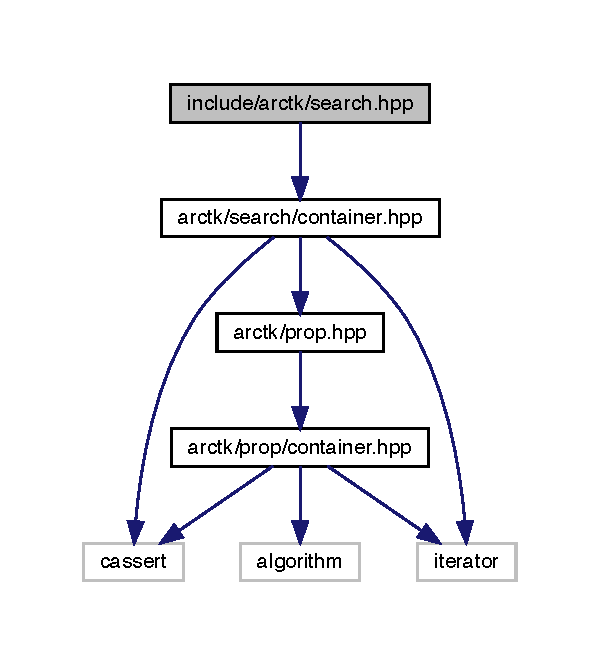
\includegraphics[width=288pt]{search_8hpp__incl}
\end{center}
\end{figure}
This graph shows which files directly or indirectly include this file\+:\nopagebreak
\begin{figure}[H]
\begin{center}
\leavevmode
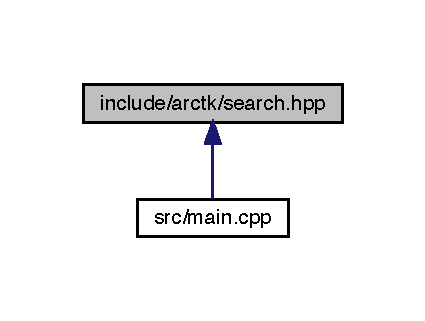
\includegraphics[width=204pt]{search_8hpp__dep__incl}
\end{center}
\end{figure}


\subsection{Detailed Description}
\begin{DoxyDate}{Date}
29/05/2018 
\end{DoxyDate}
\begin{DoxyAuthor}{Author}
Freddy Wordingham
\end{DoxyAuthor}
Collection of property functions.

\begin{DoxyDate}{Date}
29/05/2018 
\end{DoxyDate}
\begin{DoxyAuthor}{Author}
Freddy Wordingham
\end{DoxyAuthor}
Collection of search functions. 
\hypertarget{str_8hpp}{}\section{include/arctk/str.hpp File Reference}
\label{str_8hpp}\index{include/arctk/str.\+hpp@{include/arctk/str.\+hpp}}
{\ttfamily \#include $<$arctk/str/convert.\+hpp$>$}\newline
Include dependency graph for str.\+hpp\+:\nopagebreak
\begin{figure}[H]
\begin{center}
\leavevmode
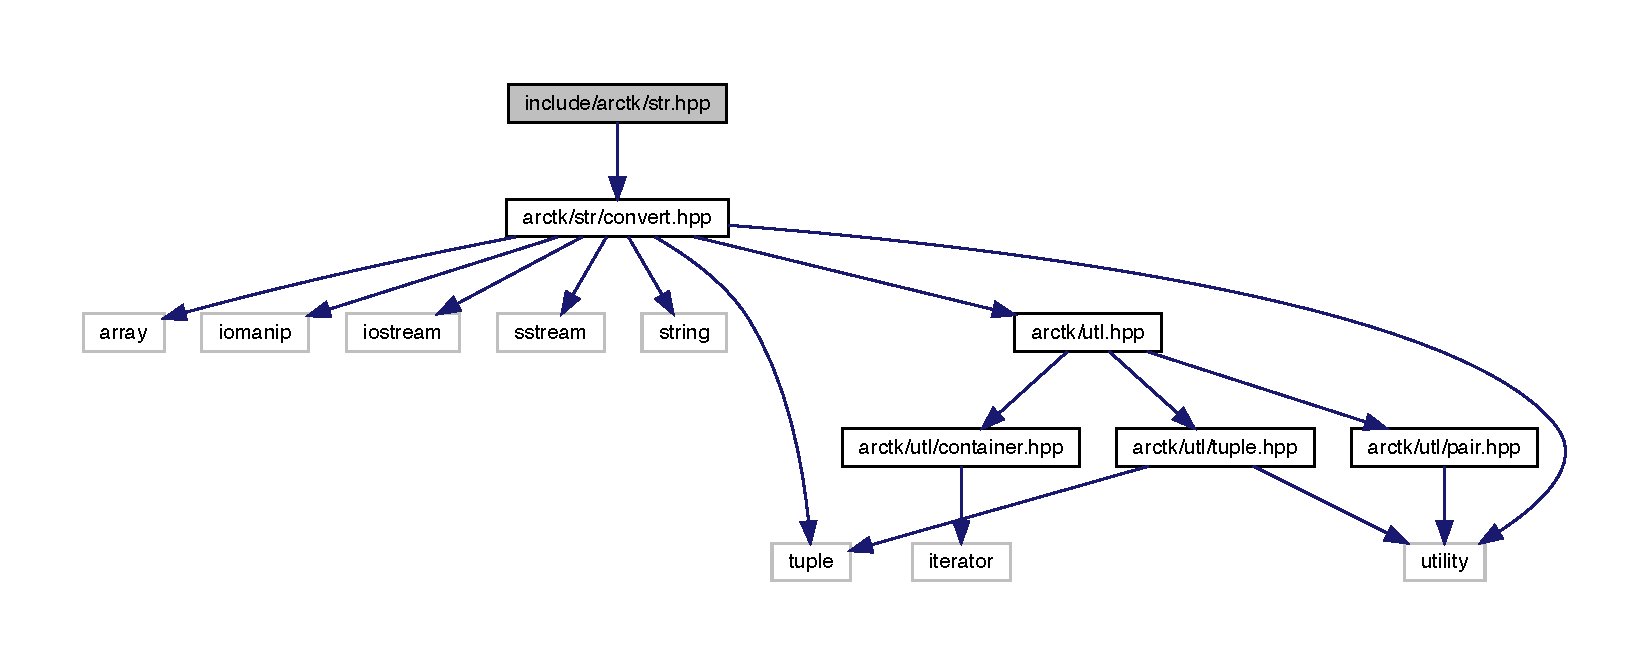
\includegraphics[width=350pt]{str_8hpp__incl}
\end{center}
\end{figure}
This graph shows which files directly or indirectly include this file\+:\nopagebreak
\begin{figure}[H]
\begin{center}
\leavevmode
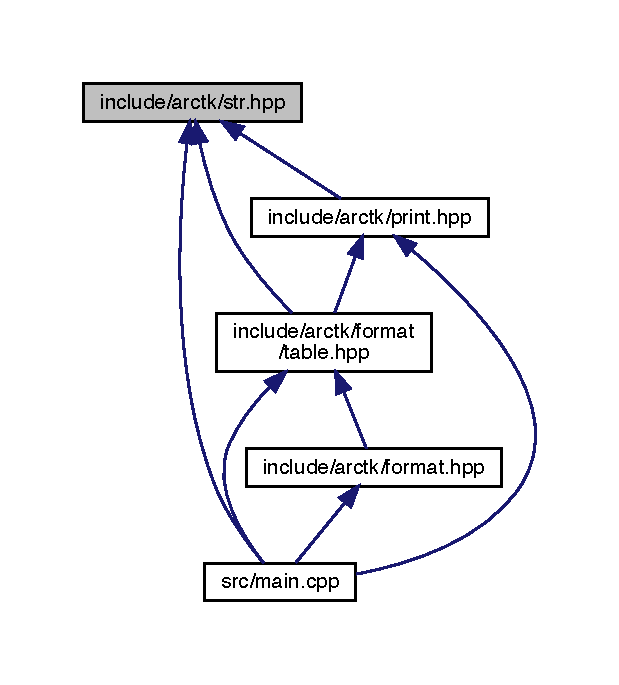
\includegraphics[width=297pt]{str_8hpp__dep__incl}
\end{center}
\end{figure}


\subsection{Detailed Description}
\begin{DoxyDate}{Date}
28/05/2018 
\end{DoxyDate}
\begin{DoxyAuthor}{Author}
Freddy Wordingham
\end{DoxyAuthor}
Collection of string functions. 
\hypertarget{convert_8hpp}{}\section{include/arctk/str/convert.hpp File Reference}
\label{convert_8hpp}\index{include/arctk/str/convert.\+hpp@{include/arctk/str/convert.\+hpp}}
{\ttfamily \#include $<$array$>$}\newline
{\ttfamily \#include $<$iomanip$>$}\newline
{\ttfamily \#include $<$iostream$>$}\newline
{\ttfamily \#include $<$sstream$>$}\newline
{\ttfamily \#include $<$string$>$}\newline
{\ttfamily \#include $<$tuple$>$}\newline
{\ttfamily \#include $<$utility$>$}\newline
{\ttfamily \#include $<$arctk/utl.\+hpp$>$}\newline
Include dependency graph for convert.\+hpp\+:\nopagebreak
\begin{figure}[H]
\begin{center}
\leavevmode
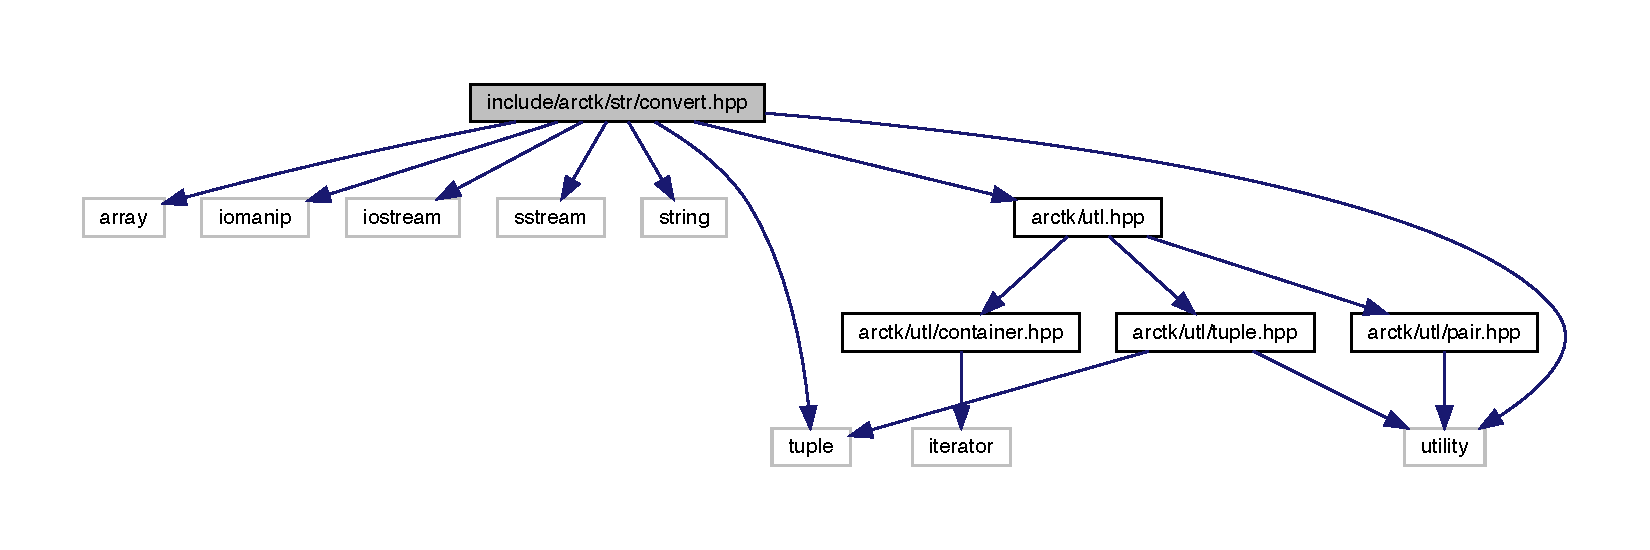
\includegraphics[width=350pt]{convert_8hpp__incl}
\end{center}
\end{figure}
This graph shows which files directly or indirectly include this file\+:\nopagebreak
\begin{figure}[H]
\begin{center}
\leavevmode
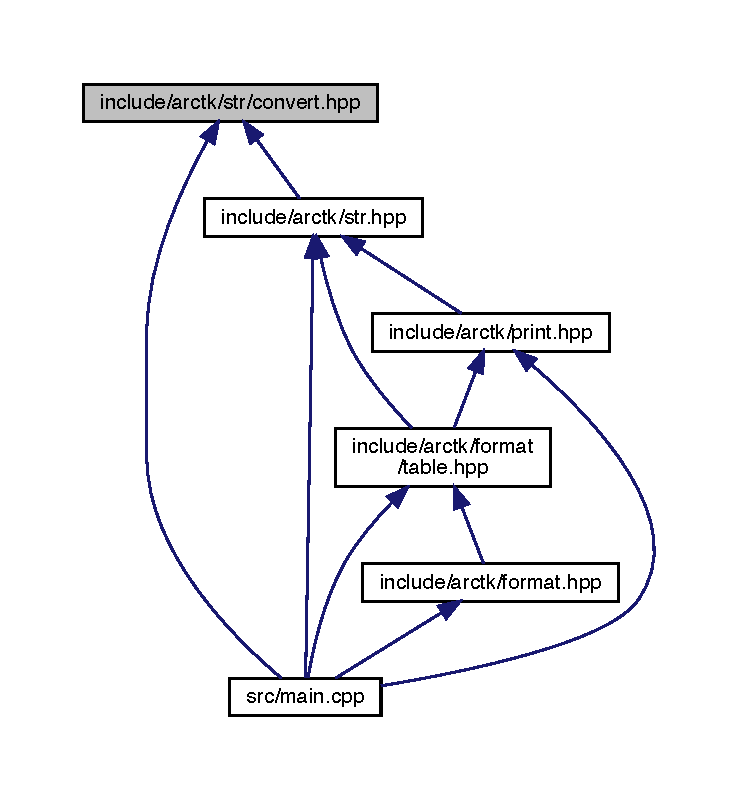
\includegraphics[width=350pt]{convert_8hpp__dep__incl}
\end{center}
\end{figure}
\subsection*{Classes}
\begin{DoxyCompactItemize}
\item 
struct \mbox{\hyperlink{structarc_1_1str_1_1_tuple_to_string}{arc\+::str\+::\+Tuple\+To\+String}}
\end{DoxyCompactItemize}
\subsection*{Namespaces}
\begin{DoxyCompactItemize}
\item 
 \mbox{\hyperlink{namespacearc}{arc}}
\begin{DoxyCompactList}\small\item\em arctk namespace \end{DoxyCompactList}\item 
 \mbox{\hyperlink{namespacearc_1_1str}{arc\+::str}}
\begin{DoxyCompactList}\small\item\em string namespace \end{DoxyCompactList}\end{DoxyCompactItemize}
\subsection*{Functions}
\begin{DoxyCompactItemize}
\item 
{\footnotesize template$<$typename C , typename T  = typename C\+::value\+\_\+type, typename I  = typename C\+::const\+\_\+iterator$>$ }\\std\+::string \mbox{\hyperlink{namespacearc_1_1str_a53e4e5a084da03d5cc8ea2d4ee8ba7d0}{arc\+::str\+::to\+\_\+string}} (const C \&cont\+\_\+, size\+\_\+t width\+\_\+=0, const std\+::string \&pre\+\_\+=\char`\"{}\{\char`\"{}, const std\+::string \&delim\+\_\+=\char`\"{}, \char`\"{}, const std\+::string \&post\+\_\+=\char`\"{}\}\char`\"{})
\item 
{\footnotesize template$<$typename A0 , typename A1 $>$ }\\std\+::string \mbox{\hyperlink{namespacearc_1_1str_a272000ff280c6447f036e80aeb3c3794}{arc\+::str\+::to\+\_\+string}} (const std\+::pair$<$ A0, A1 $>$ \&pair\+\_\+, size\+\_\+t width\+\_\+=0, const std\+::string \&pre\+\_\+=\char`\"{}(\char`\"{}, const std\+::string \&delim\+\_\+=\char`\"{}, \char`\"{}, const std\+::string \&post\+\_\+=\char`\"{})\char`\"{})
\item 
{\footnotesize template$<$typename... A$>$ }\\std\+::string \mbox{\hyperlink{namespacearc_1_1str_ab73894966cf4d5672f5c86ba7a1a1465}{arc\+::str\+::to\+\_\+string}} (const std\+::tuple$<$ A... $>$ \&tup\+\_\+, size\+\_\+t width\+\_\+=0, const std\+::string \&pre\+\_\+=\char`\"{}(\char`\"{}, const std\+::string \&delim\+\_\+=\char`\"{}, \char`\"{}, const std\+::string \&post\+\_\+=\char`\"{})\char`\"{})
\end{DoxyCompactItemize}


\subsection{Detailed Description}
\begin{DoxyDate}{Date}
28/05/2018 
\end{DoxyDate}
\begin{DoxyAuthor}{Author}
Freddy Wordingham
\end{DoxyAuthor}
Conversion to string functions. 
\hypertarget{utl_8hpp}{}\section{include/arctk/utl.hpp File Reference}
\label{utl_8hpp}\index{include/arctk/utl.\+hpp@{include/arctk/utl.\+hpp}}
{\ttfamily \#include $<$arctk/utl/container.\+hpp$>$}\newline
{\ttfamily \#include $<$arctk/utl/pair.\+hpp$>$}\newline
{\ttfamily \#include $<$arctk/utl/tuple.\+hpp$>$}\newline
Include dependency graph for utl.\+hpp\+:\nopagebreak
\begin{figure}[H]
\begin{center}
\leavevmode
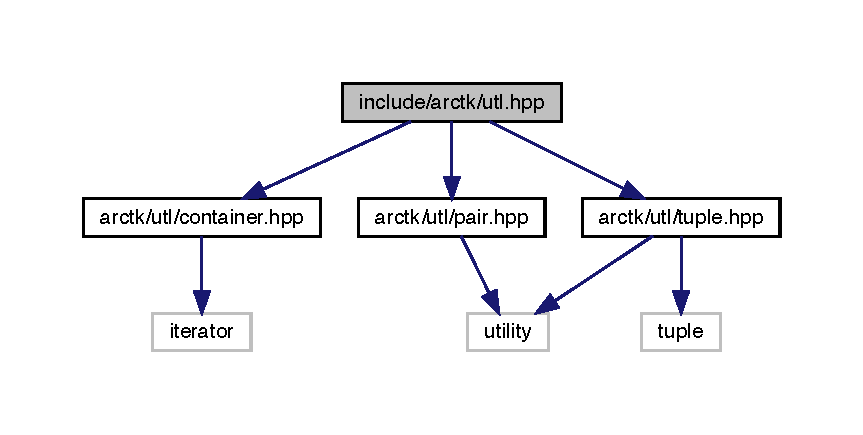
\includegraphics[width=350pt]{utl_8hpp__incl}
\end{center}
\end{figure}
This graph shows which files directly or indirectly include this file\+:\nopagebreak
\begin{figure}[H]
\begin{center}
\leavevmode
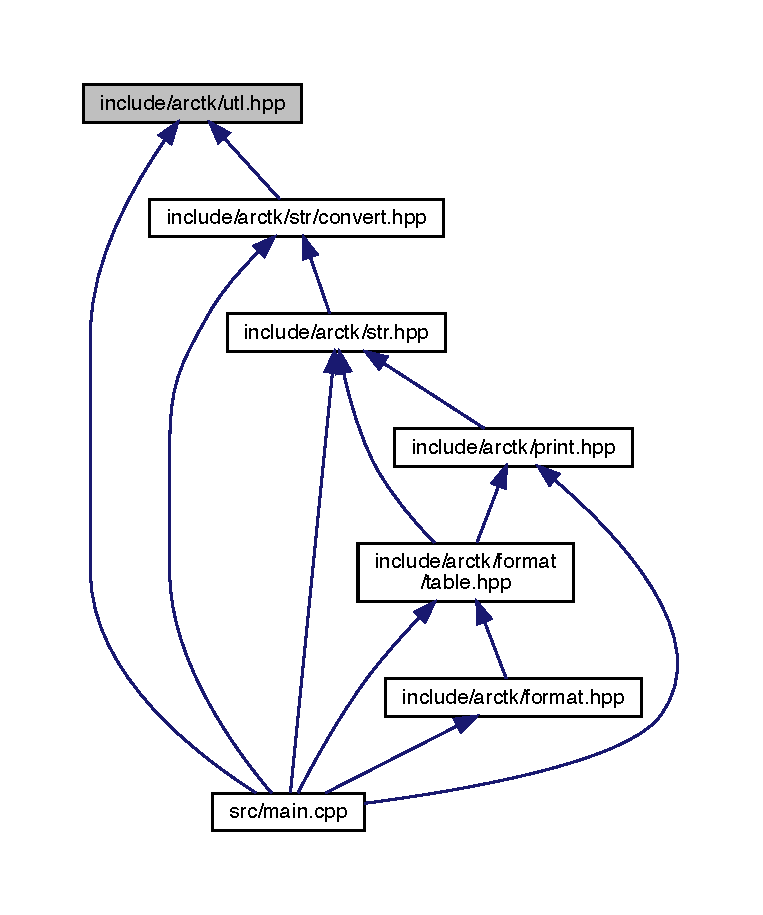
\includegraphics[width=350pt]{utl_8hpp__dep__incl}
\end{center}
\end{figure}


\subsection{Detailed Description}
\begin{DoxyDate}{Date}
28/05/2018 
\end{DoxyDate}
\begin{DoxyAuthor}{Author}
Freddy Wordingham
\end{DoxyAuthor}
Collection of utility functions. 
\hypertarget{pair_8hpp}{}\section{include/arctk/utl/pair.hpp File Reference}
\label{pair_8hpp}\index{include/arctk/utl/pair.\+hpp@{include/arctk/utl/pair.\+hpp}}
{\ttfamily \#include $<$utility$>$}\newline
Include dependency graph for pair.\+hpp\+:\nopagebreak
\begin{figure}[H]
\begin{center}
\leavevmode
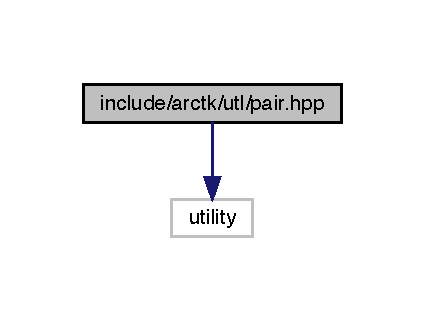
\includegraphics[width=204pt]{pair_8hpp__incl}
\end{center}
\end{figure}
This graph shows which files directly or indirectly include this file\+:\nopagebreak
\begin{figure}[H]
\begin{center}
\leavevmode
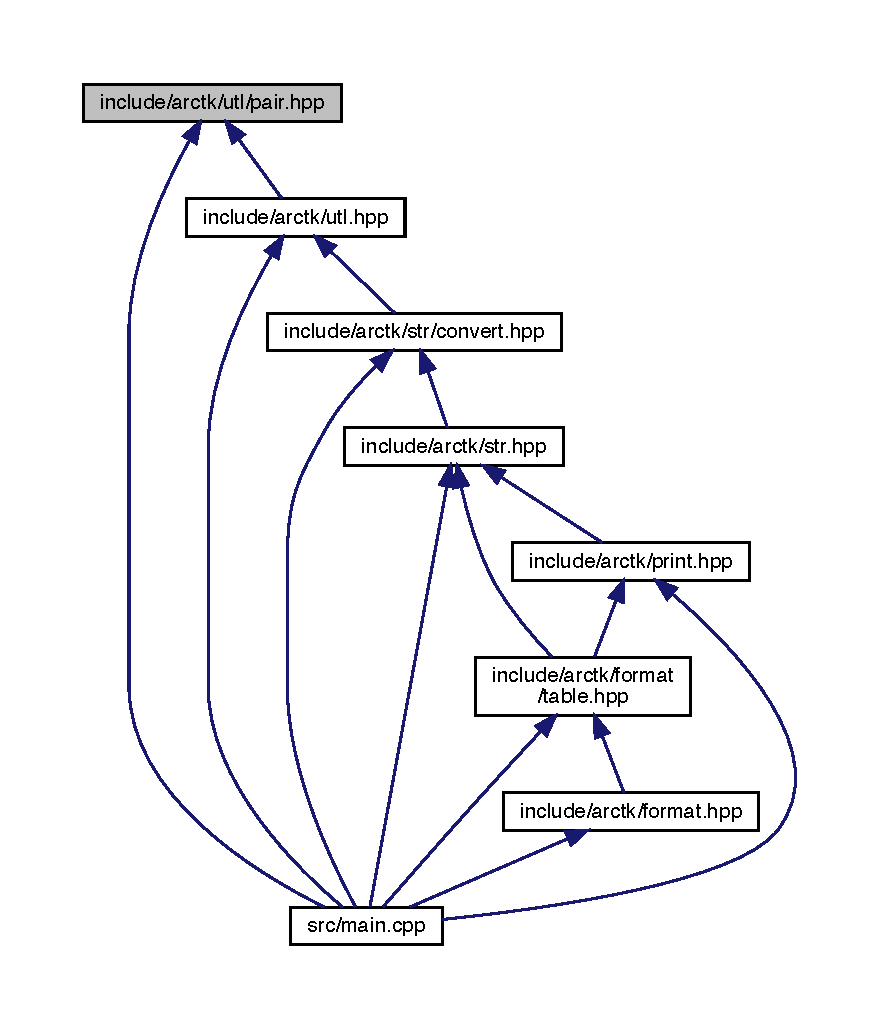
\includegraphics[width=350pt]{pair_8hpp__dep__incl}
\end{center}
\end{figure}
\subsection*{Namespaces}
\begin{DoxyCompactItemize}
\item 
 \mbox{\hyperlink{namespacearc}{arc}}
\begin{DoxyCompactList}\small\item\em arctk namespace \end{DoxyCompactList}\item 
 \mbox{\hyperlink{namespacearc_1_1utl}{arc\+::utl}}
\begin{DoxyCompactList}\small\item\em utility namespace \end{DoxyCompactList}\end{DoxyCompactItemize}
\subsection*{Functions}
\begin{DoxyCompactItemize}
\item 
{\footnotesize template$<$typename A0 , typename A1 , typename F $>$ }\\void \mbox{\hyperlink{namespacearc_1_1utl_a77c34280ea834583a0a0563e2bdc549c}{arc\+::utl\+::apply}} (std\+::pair$<$ A0, A1 $>$ \&pair\+\_\+, F func\+\_\+)
\item 
{\footnotesize template$<$typename A0 , typename A1 , typename F $>$ }\\void \mbox{\hyperlink{namespacearc_1_1utl_a887b8885b94d550a15de9eef1a70fd0b}{arc\+::utl\+::apply}} (const std\+::pair$<$ A0, A1 $>$ \&pair\+\_\+, F func\+\_\+)
\item 
{\footnotesize template$<$typename A0 , typename A1 , typename F $>$ }\\void \mbox{\hyperlink{namespacearc_1_1utl_a97b916dd6673b3b3c190b15af1719b0a}{arc\+::utl\+::apply\+\_\+with\+\_\+index}} (std\+::pair$<$ A0, A1 $>$ \&pair\+\_\+, F func\+\_\+)
\item 
{\footnotesize template$<$typename A0 , typename A1 , typename F $>$ }\\void \mbox{\hyperlink{namespacearc_1_1utl_ad77a0481ab72232b49349532b96f80fc}{arc\+::utl\+::apply\+\_\+with\+\_\+index}} (const std\+::pair$<$ A0, A1 $>$ \&pair\+\_\+, F func\+\_\+)
\end{DoxyCompactItemize}


\subsection{Detailed Description}
\begin{DoxyDate}{Date}
29/05/2018 
\end{DoxyDate}
\begin{DoxyAuthor}{Author}
Freddy Wordingham
\end{DoxyAuthor}
Pair utility functions. 
\hypertarget{tuple_8hpp}{}\section{include/arctk/utl/tuple.hpp File Reference}
\label{tuple_8hpp}\index{include/arctk/utl/tuple.\+hpp@{include/arctk/utl/tuple.\+hpp}}
{\ttfamily \#include $<$tuple$>$}\newline
{\ttfamily \#include $<$utility$>$}\newline
Include dependency graph for tuple.\+hpp\+:\nopagebreak
\begin{figure}[H]
\begin{center}
\leavevmode
\includegraphics[width=209pt]{tuple_8hpp__incl}
\end{center}
\end{figure}
This graph shows which files directly or indirectly include this file\+:\nopagebreak
\begin{figure}[H]
\begin{center}
\leavevmode
\includegraphics[width=350pt]{tuple_8hpp__dep__incl}
\end{center}
\end{figure}
\subsection*{Namespaces}
\begin{DoxyCompactItemize}
\item 
 \mbox{\hyperlink{namespacearc}{arc}}
\begin{DoxyCompactList}\small\item\em arctk namespace \end{DoxyCompactList}\item 
 \mbox{\hyperlink{namespacearc_1_1utl}{arc\+::utl}}
\begin{DoxyCompactList}\small\item\em utility namespace \end{DoxyCompactList}\end{DoxyCompactItemize}
\subsection*{Functions}
\begin{DoxyCompactItemize}
\item 
{\footnotesize template$<$typename... A, typename F , size\+\_\+t... I$>$ }\\void \mbox{\hyperlink{namespacearc_1_1utl_a5421e6de5c0a785ee70d9546d6ef0c41}{arc\+::utl\+::apply\+\_\+to\+\_\+each}} (std\+::tuple$<$ A... $>$ \&tuple\+\_\+, F func\+\_\+, std\+::index\+\_\+sequence$<$ I... $>$)
\item 
{\footnotesize template$<$typename... A, typename F $>$ }\\void \mbox{\hyperlink{namespacearc_1_1utl_af64bed0e9e6ac7220d393a1bb62f4bff}{arc\+::utl\+::apply}} (std\+::tuple$<$ A... $>$ \&tuple\+\_\+, F func\+\_\+)
\item 
{\footnotesize template$<$typename... A, typename F , size\+\_\+t... I$>$ }\\void \mbox{\hyperlink{namespacearc_1_1utl_acf59dac8c2f5eea5a6aa9875db3b07f8}{arc\+::utl\+::apply\+\_\+to\+\_\+each}} (const std\+::tuple$<$ A... $>$ \&tuple\+\_\+, F func\+\_\+, std\+::index\+\_\+sequence$<$ I... $>$)
\item 
{\footnotesize template$<$typename... A, typename F $>$ }\\void \mbox{\hyperlink{namespacearc_1_1utl_a6dadc719c6540032592f36b5c14cae27}{arc\+::utl\+::apply}} (const std\+::tuple$<$ A... $>$ \&tuple\+\_\+, F func\+\_\+)
\item 
{\footnotesize template$<$typename... A, typename F , size\+\_\+t... I$>$ }\\void \mbox{\hyperlink{namespacearc_1_1utl_a0bc38a64f17e53212169cae0a6eb23bb}{arc\+::utl\+::apply\+\_\+to\+\_\+each\+\_\+with\+\_\+index}} (std\+::tuple$<$ A... $>$ \&tuple\+\_\+, F func\+\_\+, std\+::index\+\_\+sequence$<$ I... $>$)
\item 
{\footnotesize template$<$typename... A, typename F $>$ }\\void \mbox{\hyperlink{namespacearc_1_1utl_a2658c84859917c434ff3a7f667b21eca}{arc\+::utl\+::apply\+\_\+with\+\_\+index}} (std\+::tuple$<$ A... $>$ \&tuple\+\_\+, F func\+\_\+)
\item 
{\footnotesize template$<$typename... A, typename F , size\+\_\+t... I$>$ }\\void \mbox{\hyperlink{namespacearc_1_1utl_a6330262543d471ad23a1a70ea3a47b53}{arc\+::utl\+::apply\+\_\+to\+\_\+each\+\_\+with\+\_\+index}} (const std\+::tuple$<$ A... $>$ \&tuple\+\_\+, F func\+\_\+, std\+::index\+\_\+sequence$<$ I... $>$)
\item 
{\footnotesize template$<$typename... A, typename F $>$ }\\void \mbox{\hyperlink{namespacearc_1_1utl_ae57e12a4fd6beeb3a1a40bfd461c3a87}{arc\+::utl\+::apply\+\_\+with\+\_\+index}} (const std\+::tuple$<$ A... $>$ \&tuple\+\_\+, F func\+\_\+)
\end{DoxyCompactItemize}


\subsection{Detailed Description}
\begin{DoxyDate}{Date}
28/05/2018 
\end{DoxyDate}
\begin{DoxyAuthor}{Author}
Freddy Wordingham
\end{DoxyAuthor}
Tuple utility functions. 
\hypertarget{main_8cpp}{}\section{src/main.cpp File Reference}
\label{main_8cpp}\index{src/main.\+cpp@{src/main.\+cpp}}
{\ttfamily \#include $<$arctk/config.\+hpp$>$}\newline
{\ttfamily \#include $<$arctk/constant.\+hpp$>$}\newline
{\ttfamily \#include $<$arctk/constant/math.\+hpp$>$}\newline
{\ttfamily \#include $<$arctk/constant/phys.\+hpp$>$}\newline
{\ttfamily \#include $<$arctk/format.\+hpp$>$}\newline
{\ttfamily \#include $<$arctk/format/table.\+hpp$>$}\newline
{\ttfamily \#include $<$arctk/print.\+hpp$>$}\newline
{\ttfamily \#include $<$arctk/prop.\+hpp$>$}\newline
{\ttfamily \#include $<$arctk/prop/container.\+hpp$>$}\newline
{\ttfamily \#include $<$arctk/search.\+hpp$>$}\newline
{\ttfamily \#include $<$arctk/search/container.\+hpp$>$}\newline
{\ttfamily \#include $<$arctk/str.\+hpp$>$}\newline
{\ttfamily \#include $<$arctk/str/convert.\+hpp$>$}\newline
{\ttfamily \#include $<$arctk/utl.\+hpp$>$}\newline
{\ttfamily \#include $<$arctk/utl/container.\+hpp$>$}\newline
{\ttfamily \#include $<$arctk/utl/pair.\+hpp$>$}\newline
{\ttfamily \#include $<$arctk/utl/tuple.\+hpp$>$}\newline
Include dependency graph for main.\+cpp\+:\nopagebreak
\begin{figure}[H]
\begin{center}
\leavevmode
\includegraphics[width=350pt]{main_8cpp__incl}
\end{center}
\end{figure}
\subsection*{Functions}
\begin{DoxyCompactItemize}
\item 
int \mbox{\hyperlink{main_8cpp_a3718b1cdde8158b6d3991e85fd04d50d}{main}} (const int, char $\ast$$\ast$)
\end{DoxyCompactItemize}


\subsection{Detailed Description}
\begin{DoxyDate}{Date}
15/05/2018 
\end{DoxyDate}
\begin{DoxyAuthor}{Author}
Freddy Wordingham
\end{DoxyAuthor}
Main source file of arctk. Lists all header files fo static-\/analysis. 

\subsection{Function Documentation}
\mbox{\Hypertarget{main_8cpp_a3718b1cdde8158b6d3991e85fd04d50d}\label{main_8cpp_a3718b1cdde8158b6d3991e85fd04d50d}} 
\index{main.\+cpp@{main.\+cpp}!main@{main}}
\index{main@{main}!main.\+cpp@{main.\+cpp}}
\subsubsection{\texorpdfstring{main()}{main()}}
{\footnotesize\ttfamily int main (\begin{DoxyParamCaption}\item[{const int}]{,  }\item[{char $\ast$$\ast$}]{ }\end{DoxyParamCaption})}

Main function of Arctk. Serves only as a main entity.

\begin{DoxyReturn}{Returns}
Zero upon a successful run. 
\end{DoxyReturn}

%--- End generated contents ---

% Index
\backmatter
\newpage
\phantomsection
\clearemptydoublepage
\addcontentsline{toc}{chapter}{Index}
\printindex

\end{document}
